\documentclass[twoside]{book}

% Packages required by doxygen
\usepackage{calc}
\usepackage{doxygen}
\usepackage{graphicx}
\usepackage[utf8]{inputenc}
\usepackage{makeidx}
\usepackage{multicol}
\usepackage{multirow}
\usepackage{textcomp}
\usepackage[table]{xcolor}

% Font selection
\usepackage[T1]{fontenc}
\usepackage{mathptmx}
\usepackage[scaled=.90]{helvet}
\usepackage{courier}
\usepackage{amssymb}
\usepackage{sectsty}
\renewcommand{\familydefault}{\sfdefault}
\allsectionsfont{%
  \fontseries{bc}\selectfont%
  \color{darkgray}%
}
\renewcommand{\DoxyLabelFont}{%
  \fontseries{bc}\selectfont%
  \color{darkgray}%
}

% Page & text layout
\usepackage{geometry}
\geometry{%
  a4paper,%
  top=2.5cm,%
  bottom=2.5cm,%
  left=2.5cm,%
  right=2.5cm%
}
\tolerance=750
\hfuzz=15pt
\hbadness=750
\setlength{\emergencystretch}{15pt}
\setlength{\parindent}{0cm}
\setlength{\parskip}{0.2cm}
\makeatletter
\renewcommand{\paragraph}{%
  \@startsection{paragraph}{4}{0ex}{-1.0ex}{1.0ex}{%
    \normalfont\normalsize\bfseries\SS@parafont%
  }%
}
\renewcommand{\subparagraph}{%
  \@startsection{subparagraph}{5}{0ex}{-1.0ex}{1.0ex}{%
    \normalfont\normalsize\bfseries\SS@subparafont%
  }%
}
\makeatother

% Headers & footers
\usepackage{fancyhdr}
\pagestyle{fancyplain}
\fancyhead[LE]{\fancyplain{}{\bfseries\thepage}}
\fancyhead[CE]{\fancyplain{}{}}
\fancyhead[RE]{\fancyplain{}{\bfseries\leftmark}}
\fancyhead[LO]{\fancyplain{}{\bfseries\rightmark}}
\fancyhead[CO]{\fancyplain{}{}}
\fancyhead[RO]{\fancyplain{}{\bfseries\thepage}}
\fancyfoot[LE]{\fancyplain{}{}}
\fancyfoot[CE]{\fancyplain{}{}}
\fancyfoot[RE]{\fancyplain{}{\bfseries\scriptsize Generated on Wed Sep 18 2013 14:29:04 for Watena by Doxygen }}
\fancyfoot[LO]{\fancyplain{}{\bfseries\scriptsize Generated on Wed Sep 18 2013 14:29:04 for Watena by Doxygen }}
\fancyfoot[CO]{\fancyplain{}{}}
\fancyfoot[RO]{\fancyplain{}{}}
\renewcommand{\footrulewidth}{0.4pt}
\renewcommand{\chaptermark}[1]{%
  \markboth{#1}{}%
}
\renewcommand{\sectionmark}[1]{%
  \markright{\thesection\ #1}%
}

% Indices & bibliography
\usepackage{natbib}
\usepackage[titles]{tocloft}
\setcounter{tocdepth}{3}
\setcounter{secnumdepth}{5}
\makeindex

% Hyperlinks (required, but should be loaded last)
\usepackage{ifpdf}
\ifpdf
  \usepackage[pdftex,pagebackref=true]{hyperref}
\else
  \usepackage[ps2pdf,pagebackref=true]{hyperref}
\fi
\hypersetup{%
  colorlinks=true,%
  linkcolor=blue,%
  citecolor=blue,%
  unicode%
}

% Custom commands
\newcommand{\clearemptydoublepage}{%
  \newpage{\pagestyle{empty}\cleardoublepage}%
}


%===== C O N T E N T S =====

\begin{document}

% Titlepage & ToC
\hypersetup{pageanchor=false}
\pagenumbering{roman}
\begin{titlepage}
\vspace*{7cm}
\begin{center}%
{\Large Watena }\\
\vspace*{1cm}
{\large Generated by Doxygen 1.8.4}\\
\vspace*{0.5cm}
{\small Wed Sep 18 2013 14:29:04}\\
\end{center}
\end{titlepage}
\clearemptydoublepage
\tableofcontents
\clearemptydoublepage
\pagenumbering{arabic}
\hypersetup{pageanchor=true}

%--- Begin generated contents ---
\chapter{Deprecated List}
\label{deprecated}
\hypertarget{deprecated}{}

\begin{DoxyRefList}
\item[\label{deprecated__deprecated000002}%
\hypertarget{deprecated__deprecated000002}{}%
Member \hyperlink{class_base_facebook_ab97bde45113f0c14d1c42c154e39ecf5}{Base\-Facebook\-:\-:get\-Api\-Secret} ()]
\item[\label{deprecated__deprecated000001}%
\hypertarget{deprecated__deprecated000001}{}%
Member \hyperlink{class_base_facebook_afafa43cb0a481b084ae523a04e816016}{Base\-Facebook\-:\-:set\-Api\-Secret} (\$api\-Secret)]
\end{DoxyRefList}
\chapter{Hierarchical Index}
\section{Class Hierarchy}
This inheritance list is sorted roughly, but not completely, alphabetically\-:\begin{DoxyCompactList}
\item \contentsline{section}{A\-J\-A\-X\-\_\-\-Client}{\pageref{class_a_j_a_x___client}}{}
\item \contentsline{section}{A\-J\-A\-X\-\_\-\-Request}{\pageref{class_a_j_a_x___request}}{}
\item \contentsline{section}{A\-J\-A\-X\-\_\-\-Response}{\pageref{class_a_j_a_x___response}}{}
\item \contentsline{section}{A\-J\-A\-X\-\_\-\-Selector}{\pageref{class_a_j_a_x___selector}}{}
\item \contentsline{section}{A\-J\-A\-X\-\_\-\-Server}{\pageref{class_a_j_a_x___server}}{}
\item \contentsline{section}{Base\-Facebook}{\pageref{class_base_facebook}}{}
\begin{DoxyCompactList}
\item \contentsline{section}{Facebook}{\pageref{class_facebook}}{}
\end{DoxyCompactList}
\item \contentsline{section}{Cacheable}{\pageref{class_cacheable}}{}
\item \contentsline{section}{Facebook\-Api\-Exception}{\pageref{class_facebook_api_exception}}{}
\item \contentsline{section}{html2text}{\pageref{classhtml2text}}{}
\item \contentsline{section}{I\-P\-C\-O}{\pageref{class_i_p_c_o}}{}
\item \contentsline{section}{Logger}{\pageref{class_logger}}{}
\item \contentsline{section}{O\-Auth\-Signature\-Method}{\pageref{class_o_auth_signature_method}}{}
\begin{DoxyCompactList}
\item \contentsline{section}{O\-Auth\-Signature\-Method\-\_\-\-H\-M\-A\-C\-\_\-\-S\-H\-A1}{\pageref{class_o_auth_signature_method___h_m_a_c___s_h_a1}}{}
\item \contentsline{section}{O\-Auth\-Signature\-Method\-\_\-\-P\-L\-A\-I\-N\-T\-E\-X\-T}{\pageref{class_o_auth_signature_method___p_l_a_i_n_t_e_x_t}}{}
\item \contentsline{section}{O\-Auth\-Signature\-Method\-\_\-\-R\-S\-A\-\_\-\-S\-H\-A1}{\pageref{class_o_auth_signature_method___r_s_a___s_h_a1}}{}
\end{DoxyCompactList}
\item \contentsline{section}{Request}{\pageref{class_request}}{}
\item \contentsline{section}{Session\-Guard}{\pageref{class_session_guard}}{}
\item \contentsline{section}{Template\-File}{\pageref{class_template_file}}{}
\item \contentsline{section}{Template\-Loader}{\pageref{class_template_loader}}{}
\item \contentsline{section}{T\-M\-X\-\_\-\-Ajax\-Page}{\pageref{class_t_m_x___ajax_page}}{}
\end{DoxyCompactList}

\chapter{Class Index}
\section{Class List}
Here are the classes, structs, unions and interfaces with brief descriptions\-:\begin{DoxyCompactList}
\item\contentsline{section}{\hyperlink{class_a_j_a_x___client}{A\-J\-A\-X\-\_\-\-Client} }{\pageref{class_a_j_a_x___client}}{}
\item\contentsline{section}{\hyperlink{class_a_j_a_x___request}{A\-J\-A\-X\-\_\-\-Request} }{\pageref{class_a_j_a_x___request}}{}
\item\contentsline{section}{\hyperlink{class_a_j_a_x___server}{A\-J\-A\-X\-\_\-\-Server} }{\pageref{class_a_j_a_x___server}}{}
\item\contentsline{section}{\hyperlink{class_base_facebook}{Base\-Facebook} }{\pageref{class_base_facebook}}{}
\item\contentsline{section}{\hyperlink{class_cacheable}{Cacheable} }{\pageref{class_cacheable}}{}
\item\contentsline{section}{\hyperlink{class_callback}{Callback} }{\pageref{class_callback}}{}
\item\contentsline{section}{\hyperlink{class_callback_model}{Callback\-Model} }{\pageref{class_callback_model}}{}
\item\contentsline{section}{\hyperlink{class_encoding}{Encoding} }{\pageref{class_encoding}}{}
\item\contentsline{section}{\hyperlink{class_facebook}{Facebook} }{\pageref{class_facebook}}{}
\item\contentsline{section}{\hyperlink{class_facebook_api_exception}{Facebook\-Api\-Exception} }{\pageref{class_facebook_api_exception}}{}
\item\contentsline{section}{\hyperlink{classhtml2text}{html2text} }{\pageref{classhtml2text}}{}
\item\contentsline{section}{\hyperlink{class_html_model}{Html\-Model} }{\pageref{class_html_model}}{}
\item\contentsline{section}{\hyperlink{class_i_p_c_o}{I\-P\-C\-O} }{\pageref{class_i_p_c_o}}{}
\item\contentsline{section}{\hyperlink{class_j_s_function}{J\-S\-Function} }{\pageref{class_j_s_function}}{}
\item\contentsline{section}{\hyperlink{class_logger}{Logger} }{\pageref{class_logger}}{}
\item\contentsline{section}{\hyperlink{class_minifie_css_view}{Minifie\-Css\-View} }{\pageref{class_minifie_css_view}}{}
\item\contentsline{section}{\hyperlink{class_minifie_js_view}{Minifie\-Js\-View} }{\pageref{class_minifie_js_view}}{}
\item\contentsline{section}{\hyperlink{class_o_auth_signature_method}{O\-Auth\-Signature\-Method} }{\pageref{class_o_auth_signature_method}}{}
\item\contentsline{section}{\hyperlink{class_o_auth_signature_method___h_m_a_c___s_h_a1}{O\-Auth\-Signature\-Method\-\_\-\-H\-M\-A\-C\-\_\-\-S\-H\-A1} }{\pageref{class_o_auth_signature_method___h_m_a_c___s_h_a1}}{}
\item\contentsline{section}{\hyperlink{class_o_auth_signature_method___p_l_a_i_n_t_e_x_t}{O\-Auth\-Signature\-Method\-\_\-\-P\-L\-A\-I\-N\-T\-E\-X\-T} }{\pageref{class_o_auth_signature_method___p_l_a_i_n_t_e_x_t}}{}
\item\contentsline{section}{\hyperlink{class_o_auth_signature_method___r_s_a___s_h_a1}{O\-Auth\-Signature\-Method\-\_\-\-R\-S\-A\-\_\-\-S\-H\-A1} }{\pageref{class_o_auth_signature_method___r_s_a___s_h_a1}}{}
\item\contentsline{section}{\hyperlink{class_request}{Request} }{\pageref{class_request}}{}
\item\contentsline{section}{\hyperlink{class_session_guard}{Session\-Guard} }{\pageref{class_session_guard}}{}
\item\contentsline{section}{\hyperlink{class_template_file}{Template\-File} }{\pageref{class_template_file}}{}
\item\contentsline{section}{\hyperlink{class_template_loader}{Template\-Loader} }{\pageref{class_template_loader}}{}
\item\contentsline{section}{\hyperlink{class_theme_file_model}{Theme\-File\-Model} }{\pageref{class_theme_file_model}}{}
\item\contentsline{section}{\hyperlink{class_view}{View} }{\pageref{class_view}}{}
\end{DoxyCompactList}

\chapter{Class Documentation}
\hypertarget{class_a_j_a_x___client}{\section{A\-J\-A\-X\-\_\-\-Client Class Reference}
\label{class_a_j_a_x___client}\index{A\-J\-A\-X\-\_\-\-Client@{A\-J\-A\-X\-\_\-\-Client}}
}
\subsection*{Public Member Functions}
\begin{DoxyCompactItemize}
\item 
\hyperlink{class_a_j_a_x___client_abbf82c39947b3452ff57b37859acc2da}{\-\_\-\-\_\-construct} (\$s\-Javascript\-Link=null)
\item 
\hyperlink{class_a_j_a_x___client_a6fe317ebce44e13e98c9ab24a61edbfe}{register\-Request} (\hyperlink{class_a_j_a_x___request}{A\-J\-A\-X\-\_\-\-Request} \$o\-Request)
\item 
\hyperlink{class_a_j_a_x___client_aa979a925e3be08d3000522d672850a14}{get\-Javascript\-Link} ()
\item 
\hyperlink{class_a_j_a_x___client_a01704f2374d8db6ee806d774958b66d9}{get\-Output} ()
\end{DoxyCompactItemize}


\subsection{Detailed Description}
Client A\-J\-A\-X class that processes all registered requests

\begin{DoxyAuthor}{Author}
Voet Jelle 
\end{DoxyAuthor}
\begin{DoxyVersion}{Version}
1.\-0.\-0 beta 
\end{DoxyVersion}


\subsection{Constructor \& Destructor Documentation}
\hypertarget{class_a_j_a_x___client_abbf82c39947b3452ff57b37859acc2da}{\index{A\-J\-A\-X\-\_\-\-Client@{A\-J\-A\-X\-\_\-\-Client}!\-\_\-\-\_\-construct@{\-\_\-\-\_\-construct}}
\index{\-\_\-\-\_\-construct@{\-\_\-\-\_\-construct}!AJAX_Client@{A\-J\-A\-X\-\_\-\-Client}}
\subsubsection[{\-\_\-\-\_\-construct}]{\setlength{\rightskip}{0pt plus 5cm}A\-J\-A\-X\-\_\-\-Client\-::\-\_\-\-\_\-construct (
\begin{DoxyParamCaption}
\item[{}]{\$s\-Javascript\-Link = {\ttfamily null}}
\end{DoxyParamCaption}
)}}\label{class_a_j_a_x___client_abbf82c39947b3452ff57b37859acc2da}
Create a new client instance. If no javascriptlink is provided, you take responsability to load the ajax.\-js file. If indeed a links is provided, make sure it's absolute, no more processing will be done.


\begin{DoxyParams}[1]{Parameters}
string & {\em \$s\-Javascript\-Link} & \\
\hline
\end{DoxyParams}


\subsection{Member Function Documentation}
\hypertarget{class_a_j_a_x___client_aa979a925e3be08d3000522d672850a14}{\index{A\-J\-A\-X\-\_\-\-Client@{A\-J\-A\-X\-\_\-\-Client}!get\-Javascript\-Link@{get\-Javascript\-Link}}
\index{get\-Javascript\-Link@{get\-Javascript\-Link}!AJAX_Client@{A\-J\-A\-X\-\_\-\-Client}}
\subsubsection[{get\-Javascript\-Link}]{\setlength{\rightskip}{0pt plus 5cm}A\-J\-A\-X\-\_\-\-Client\-::get\-Javascript\-Link (
\begin{DoxyParamCaption}
{}
\end{DoxyParamCaption}
)}}\label{class_a_j_a_x___client_aa979a925e3be08d3000522d672850a14}
Return the javascript-\/links passed to the constructor.

\begin{DoxyReturn}{Returns}
string 
\end{DoxyReturn}
\hypertarget{class_a_j_a_x___client_a01704f2374d8db6ee806d774958b66d9}{\index{A\-J\-A\-X\-\_\-\-Client@{A\-J\-A\-X\-\_\-\-Client}!get\-Output@{get\-Output}}
\index{get\-Output@{get\-Output}!AJAX_Client@{A\-J\-A\-X\-\_\-\-Client}}
\subsubsection[{get\-Output}]{\setlength{\rightskip}{0pt plus 5cm}A\-J\-A\-X\-\_\-\-Client\-::get\-Output (
\begin{DoxyParamCaption}
{}
\end{DoxyParamCaption}
)}}\label{class_a_j_a_x___client_a01704f2374d8db6ee806d774958b66d9}
Process all registered requests


\begin{DoxyParams}[1]{Parameters}
bool & {\em \$b\-Echo} & choose if all data should be auto-\/echo-\/ed \\
\hline
\end{DoxyParams}
\begin{DoxyReturn}{Returns}
string 
\end{DoxyReturn}
\hypertarget{class_a_j_a_x___client_a6fe317ebce44e13e98c9ab24a61edbfe}{\index{A\-J\-A\-X\-\_\-\-Client@{A\-J\-A\-X\-\_\-\-Client}!register\-Request@{register\-Request}}
\index{register\-Request@{register\-Request}!AJAX_Client@{A\-J\-A\-X\-\_\-\-Client}}
\subsubsection[{register\-Request}]{\setlength{\rightskip}{0pt plus 5cm}A\-J\-A\-X\-\_\-\-Client\-::register\-Request (
\begin{DoxyParamCaption}
\item[{{\bf A\-J\-A\-X\-\_\-\-Request}}]{\$o\-Request}
\end{DoxyParamCaption}
)}}\label{class_a_j_a_x___client_a6fe317ebce44e13e98c9ab24a61edbfe}
Register a new request


\begin{DoxyParams}[1]{Parameters}
\hyperlink{class_a_j_a_x___request}{A\-J\-A\-X\-\_\-\-Request} & {\em \$o\-Request} & \\
\hline
\end{DoxyParams}


The documentation for this class was generated from the following file\-:\begin{DoxyCompactItemize}
\item 
ajax\-\_\-client.\-php\end{DoxyCompactItemize}

\hypertarget{class_a_j_a_x___request}{\section{A\-J\-A\-X\-\_\-\-Request Class Reference}
\label{class_a_j_a_x___request}\index{A\-J\-A\-X\-\_\-\-Request@{A\-J\-A\-X\-\_\-\-Request}}
}


Inherits Object.

\subsection*{Public Member Functions}
\begin{DoxyCompactItemize}
\item 
\hyperlink{class_a_j_a_x___request_ac2740cb109bab254475f45cde36a7c51}{\-\_\-\-\_\-construct} (\$s\-Function, \$n\-Arg\-Count=0)
\item 
\hyperlink{class_a_j_a_x___request_a46eda702ebc8b0c5b40582faa54d4430}{set\-Url} (\$s\-Url)
\item 
\hyperlink{class_a_j_a_x___request_a155a570af13c465ce28a1db0600a15ed}{set\-Value} (\$s\-Name, \$s\-Value)
\item 
\hyperlink{class_a_j_a_x___request_a18241531ebf16a4314b84e3e6c59b807}{set\-Arg\-Count} (\$n\-Arg\-Count)
\item 
\hyperlink{class_a_j_a_x___request_a56516da4748a2fb29e8043fa05727ff0}{get\-Output} ()
\end{DoxyCompactItemize}
\subsection*{Additional Inherited Members}


\subsection{Detailed Description}
Class that provides the data that are uwed when requesting some ajax-\/data

\begin{DoxyAuthor}{Author}
Voet Jelle -\/ To\-Mo-\/design 
\end{DoxyAuthor}
\begin{DoxyVersion}{Version}
2.\-0.\-1 beta
\end{DoxyVersion}
\subsubsection*{V\-E\-R\-S\-I\-O\-N-\/\-L\-O\-G }

1-\/8-\/2010\-: 2.\-0.\-0 =$>$ 2.\-0.\-1
\begin{DoxyItemize}
\item Made the generated javascript-\/function call a bit smaller
\item Fixed a possible bug when using a variable U\-R\-L
\end{DoxyItemize}

30-\/7-\/2010\-: 1.\-0.\-0 =$>$ 2.\-0.\-0
\begin{DoxyItemize}
\item Revamped the processed output
\item Added J\-S\-O\-N
\item Added rawurlencode/encode\-U\-R\-I\-Component
\item Made the output somewhat smaller 
\end{DoxyItemize}

\subsection{Constructor \& Destructor Documentation}
\hypertarget{class_a_j_a_x___request_ac2740cb109bab254475f45cde36a7c51}{\index{A\-J\-A\-X\-\_\-\-Request@{A\-J\-A\-X\-\_\-\-Request}!\-\_\-\-\_\-construct@{\-\_\-\-\_\-construct}}
\index{\-\_\-\-\_\-construct@{\-\_\-\-\_\-construct}!AJAX_Request@{A\-J\-A\-X\-\_\-\-Request}}
\subsubsection[{\-\_\-\-\_\-construct}]{\setlength{\rightskip}{0pt plus 5cm}A\-J\-A\-X\-\_\-\-Request\-::\-\_\-\-\_\-construct (
\begin{DoxyParamCaption}
\item[{}]{\$s\-Function, }
\item[{}]{\$n\-Arg\-Count = {\ttfamily 0}}
\end{DoxyParamCaption}
)}}\label{class_a_j_a_x___request_ac2740cb109bab254475f45cde36a7c51}
Create a new request


\begin{DoxyParams}[1]{Parameters}
string & {\em \$s\-U\-R\-L} & the request \hyperlink{class_u_r_i}{U\-R\-I} \\
\hline
mixed & {\em \$\-P\-H\-P\-Callback} & the php function to be called on the server to process the request \\
\hline
string & {\em \$s\-J\-S\-Callback} & the javascript function that you can call on your html-\/page \\
\hline
int & {\em \$n\-Arg\-Count} & the number of arguments you can set in your javascript-\//php-\/function \\
\hline
\end{DoxyParams}


\subsection{Member Function Documentation}
\hypertarget{class_a_j_a_x___request_a56516da4748a2fb29e8043fa05727ff0}{\index{A\-J\-A\-X\-\_\-\-Request@{A\-J\-A\-X\-\_\-\-Request}!get\-Output@{get\-Output}}
\index{get\-Output@{get\-Output}!AJAX_Request@{A\-J\-A\-X\-\_\-\-Request}}
\subsubsection[{get\-Output}]{\setlength{\rightskip}{0pt plus 5cm}A\-J\-A\-X\-\_\-\-Request\-::get\-Output (
\begin{DoxyParamCaption}
{}
\end{DoxyParamCaption}
)}}\label{class_a_j_a_x___request_a56516da4748a2fb29e8043fa05727ff0}
Process this request-\/data

\begin{DoxyReturn}{Returns}
string 
\end{DoxyReturn}
\hypertarget{class_a_j_a_x___request_a18241531ebf16a4314b84e3e6c59b807}{\index{A\-J\-A\-X\-\_\-\-Request@{A\-J\-A\-X\-\_\-\-Request}!set\-Arg\-Count@{set\-Arg\-Count}}
\index{set\-Arg\-Count@{set\-Arg\-Count}!AJAX_Request@{A\-J\-A\-X\-\_\-\-Request}}
\subsubsection[{set\-Arg\-Count}]{\setlength{\rightskip}{0pt plus 5cm}A\-J\-A\-X\-\_\-\-Request\-::set\-Arg\-Count (
\begin{DoxyParamCaption}
\item[{}]{\$n\-Arg\-Count}
\end{DoxyParamCaption}
)}}\label{class_a_j_a_x___request_a18241531ebf16a4314b84e3e6c59b807}
Set the number of arguments you can set for your javascript-\//php-\/function


\begin{DoxyParams}[1]{Parameters}
int & {\em \$n\-Arg\-Count} & \\
\hline
\end{DoxyParams}
\hypertarget{class_a_j_a_x___request_a46eda702ebc8b0c5b40582faa54d4430}{\index{A\-J\-A\-X\-\_\-\-Request@{A\-J\-A\-X\-\_\-\-Request}!set\-Url@{set\-Url}}
\index{set\-Url@{set\-Url}!AJAX_Request@{A\-J\-A\-X\-\_\-\-Request}}
\subsubsection[{set\-Url}]{\setlength{\rightskip}{0pt plus 5cm}A\-J\-A\-X\-\_\-\-Request\-::set\-Url (
\begin{DoxyParamCaption}
\item[{}]{\$s\-Url}
\end{DoxyParamCaption}
)}}\label{class_a_j_a_x___request_a46eda702ebc8b0c5b40582faa54d4430}
Set a fixed url that will be called when the function is invoked.


\begin{DoxyParams}[1]{Parameters}
string & {\em \$s\-Url} & \\
\hline
\end{DoxyParams}
\hypertarget{class_a_j_a_x___request_a155a570af13c465ce28a1db0600a15ed}{\index{A\-J\-A\-X\-\_\-\-Request@{A\-J\-A\-X\-\_\-\-Request}!set\-Value@{set\-Value}}
\index{set\-Value@{set\-Value}!AJAX_Request@{A\-J\-A\-X\-\_\-\-Request}}
\subsubsection[{set\-Value}]{\setlength{\rightskip}{0pt plus 5cm}A\-J\-A\-X\-\_\-\-Request\-::set\-Value (
\begin{DoxyParamCaption}
\item[{}]{\$s\-Name, }
\item[{}]{\$s\-Value}
\end{DoxyParamCaption}
)}}\label{class_a_j_a_x___request_a155a570af13c465ce28a1db0600a15ed}
Set a static value to be processed by this request


\begin{DoxyParams}[1]{Parameters}
string & {\em \$s\-Name} & \\
\hline
string & {\em \$s\-Value} & \\
\hline
\end{DoxyParams}


The documentation for this class was generated from the following file\-:\begin{DoxyCompactItemize}
\item 
ajax\-\_\-request.\-php\end{DoxyCompactItemize}

\hypertarget{class_a_j_a_x___response}{\section{A\-J\-A\-X\-\_\-\-Response Class Reference}
\label{class_a_j_a_x___response}\index{A\-J\-A\-X\-\_\-\-Response@{A\-J\-A\-X\-\_\-\-Response}}
}
\subsection*{Public Member Functions}
\begin{DoxyCompactItemize}
\item 
\hyperlink{class_a_j_a_x___response_ad375f00a3cb840edc05a9bd76a018306}{\-\_\-\-\_\-construct} (\$m\-H\-T\-M\-L\-Callback=null)
\item 
\hyperlink{class_a_j_a_x___response_aaf1fce395bcbe3abf2b468900269b847}{Add\-Code} (\$s\-Code, \$b\-Is\-Encapsulated=false)
\item 
\hyperlink{class_a_j_a_x___response_a88ef970898b2eaa6f1e00cc2f8ab525d}{Alert} (\$s\-Text)
\item 
\hyperlink{class_a_j_a_x___response_acd8296b7efd8f5a68f9a01b55b743b78}{Call\-Function} (\$s\-Function, array \$a\-Param=array())
\item 
\hyperlink{class_a_j_a_x___response_add7ea7d572b0d9dc1667e1647c3afbf6}{D\-O\-M\-Change\-By\-I\-D} (\$s\-I\-D, \$s\-H\-T\-M\-L, \$b\-Append=false)
\item 
\hyperlink{class_a_j_a_x___response_a07eaac9c29789b66c057e91000fb6154}{D\-O\-M\-Change} (T\-M\-X\-\_\-\-Selector \$o\-Selector, \$s\-H\-T\-M\-L, \$b\-Append=false)
\item 
\hyperlink{class_a_j_a_x___response_a1fa313b00bf5d79b31995f6ba7e5118a}{D\-O\-M\-Clean\-By\-I\-D} (\$s\-I\-D)
\item 
\hyperlink{class_a_j_a_x___response_a4e50a8d73c499058854b6ef469487a2f}{D\-O\-M\-Clean} (T\-M\-X\-\_\-\-Selector \$o\-Selector)
\item 
\hyperlink{class_a_j_a_x___response_a2f63ac10071f1df881cfd6832ff2d97e}{D\-O\-M\-Remove\-By\-I\-D} (\$s\-I\-D)
\item 
\hyperlink{class_a_j_a_x___response_ac23f48ef808f969afbc2f21204430584}{D\-O\-M\-Remove} (T\-M\-X\-\_\-\-Selector \$o\-Selector)
\item 
\hyperlink{class_a_j_a_x___response_aee268771716be54ef20ed7e5518745ca}{Style\-Change\-By\-I\-D} (\$s\-I\-D, \$s\-P\-Name, \$s\-P\-Value)
\item 
\hyperlink{class_a_j_a_x___response_a7a8236facfbbb8af103eef5b597e4bbe}{Style\-Change} (T\-M\-X\-\_\-\-Selector \$o\-Selector, \$s\-P\-Name, \$s\-P\-Value)
\item 
\hyperlink{class_a_j_a_x___response_a83aedd965664793eca47a68de5ac1273}{Class\-Change\-By\-I\-D} (\$s\-I\-D, \$s\-Class)
\item 
\hyperlink{class_a_j_a_x___response_a07e89d4407b8c3d2ace81fd5cb162be5}{Class\-Change} (T\-M\-X\-\_\-\-Selector \$o\-Selector, \$s\-Class)
\item 
\hyperlink{class_a_j_a_x___response_a698c3b7ce0a35fb6dfc31f13073c8fa2}{Add\-J\-S\-File} (\$s\-New\-File)
\item 
\hyperlink{class_a_j_a_x___response_a0a9d5da413c619c7d2820573da104e3a}{Replace\-J\-S\-File} (\$s\-Old\-File, \$s\-New\-File)
\item 
\hyperlink{class_a_j_a_x___response_aeebbe6e31801e025b95b56a5fcff0850}{Remove\-J\-S\-File} (\$s\-Old\-File)
\item 
\hyperlink{class_a_j_a_x___response_a95a747316bd4618b45d438a8bea385f4}{Add\-C\-S\-S\-File} (\$s\-New\-File)
\item 
\hyperlink{class_a_j_a_x___response_a020923f6c33bf4201b0ee0b7509208c3}{Replace\-C\-S\-S\-File} (\$s\-Old\-File, \$s\-New\-File)
\item 
\hyperlink{class_a_j_a_x___response_aca7ea3ab30272291eafe98d41b602700}{Remove\-C\-S\-S\-File} (\$s\-Old\-File)
\item 
\hyperlink{class_a_j_a_x___response_aa23febfae44d7e28875d88dbcd1cd305}{Process} (\$b\-Echo=true)
\end{DoxyCompactItemize}
\subsection*{Static Public Member Functions}
\begin{DoxyCompactItemize}
\item 
static \hyperlink{class_a_j_a_x___response_ad3c0f052bfa7658aa4b8e1dfa1224496}{Create\-Error\-Response} (\$n\-Code, \$s\-Message)
\item 
static \hyperlink{class_a_j_a_x___response_a1dc591d51f6abe3a7026a38efdb2e45c}{Add\-Slashes} (\$s\-Data)
\end{DoxyCompactItemize}


\subsection{Detailed Description}
Response class, that will be used to format the data that is to be send back to the server

\begin{DoxyAuthor}{Author}
Voet Jelle -\/ To\-Mo-\/design 
\end{DoxyAuthor}
\begin{DoxyVersion}{Version}
2.\-0.\-3 beta
\end{DoxyVersion}
\subsubsection*{V\-E\-R\-S\-I\-O\-N-\/\-L\-O\-G }

31-\/8-\/2010\-: 2.\-0.\-2 =$>$ 2.\-0.\-3
\begin{DoxyItemize}
\item Added sequential logic
\end{DoxyItemize}

1-\/8-\/2010\-: 2.\-0.\-0 =$>$ 2.\-0.\-2
\begin{DoxyItemize}
\item Remove whitespaces when parsing H\-T\-M\-L2\-D\-O\-M
\item Added the entity-\/lists when parsing H\-T\-M\-L2\-D\-O\-M
\end{DoxyItemize}

30-\/7-\/2010\-: 2.\-0.\-0 =$>$ 1.\-0.\-0
\begin{DoxyItemize}
\item Completely revamped everything (backwards compatibility-\/break)
\item No longer use 'inner\-H\-T\-M\-L' in favor of D\-O\-M-\/manipulation
\item Usage of J\-S\-O\-N
\item Automated parsing, ... no longer sending data trough string manipulation
\item Integrated the T\-M\-X\-\_\-\-Selector class for more advanced selection options
\item Add\-Code is \mbox{[}D\-E\-P\-R\-E\-C\-A\-T\-E\-D\mbox{]}, will no longer work and will trigger an error 
\end{DoxyItemize}

\subsection{Constructor \& Destructor Documentation}
\hypertarget{class_a_j_a_x___response_ad375f00a3cb840edc05a9bd76a018306}{\index{A\-J\-A\-X\-\_\-\-Response@{A\-J\-A\-X\-\_\-\-Response}!\-\_\-\-\_\-construct@{\-\_\-\-\_\-construct}}
\index{\-\_\-\-\_\-construct@{\-\_\-\-\_\-construct}!AJAX_Response@{A\-J\-A\-X\-\_\-\-Response}}
\subsubsection[{\-\_\-\-\_\-construct}]{\setlength{\rightskip}{0pt plus 5cm}A\-J\-A\-X\-\_\-\-Response\-::\-\_\-\-\_\-construct (
\begin{DoxyParamCaption}
\item[{}]{\$m\-H\-T\-M\-L\-Callback = {\ttfamily null}}
\end{DoxyParamCaption}
)}}\label{class_a_j_a_x___response_ad375f00a3cb840edc05a9bd76a018306}
Create a new Response object with a default state 

\subsection{Member Function Documentation}
\hypertarget{class_a_j_a_x___response_aaf1fce395bcbe3abf2b468900269b847}{\index{A\-J\-A\-X\-\_\-\-Response@{A\-J\-A\-X\-\_\-\-Response}!Add\-Code@{Add\-Code}}
\index{Add\-Code@{Add\-Code}!AJAX_Response@{A\-J\-A\-X\-\_\-\-Response}}
\subsubsection[{Add\-Code}]{\setlength{\rightskip}{0pt plus 5cm}A\-J\-A\-X\-\_\-\-Response\-::\-Add\-Code (
\begin{DoxyParamCaption}
\item[{}]{\$s\-Code, }
\item[{}]{\$b\-Is\-Encapsulated = {\ttfamily false}}
\end{DoxyParamCaption}
)}}\label{class_a_j_a_x___response_aaf1fce395bcbe3abf2b468900269b847}
Add some plain javascript-\/code to be executed on the client !!! D\-E\-P\-R\-E\-C\-A\-T\-E\-D \hypertarget{class_a_j_a_x___response_a95a747316bd4618b45d438a8bea385f4}{\index{A\-J\-A\-X\-\_\-\-Response@{A\-J\-A\-X\-\_\-\-Response}!Add\-C\-S\-S\-File@{Add\-C\-S\-S\-File}}
\index{Add\-C\-S\-S\-File@{Add\-C\-S\-S\-File}!AJAX_Response@{A\-J\-A\-X\-\_\-\-Response}}
\subsubsection[{Add\-C\-S\-S\-File}]{\setlength{\rightskip}{0pt plus 5cm}A\-J\-A\-X\-\_\-\-Response\-::\-Add\-C\-S\-S\-File (
\begin{DoxyParamCaption}
\item[{}]{\$s\-New\-File}
\end{DoxyParamCaption}
)}}\label{class_a_j_a_x___response_a95a747316bd4618b45d438a8bea385f4}
Add a new C\-S\-S file


\begin{DoxyParams}[1]{Parameters}
string & {\em \$s\-New\-File} & \\
\hline
\end{DoxyParams}
\hypertarget{class_a_j_a_x___response_a698c3b7ce0a35fb6dfc31f13073c8fa2}{\index{A\-J\-A\-X\-\_\-\-Response@{A\-J\-A\-X\-\_\-\-Response}!Add\-J\-S\-File@{Add\-J\-S\-File}}
\index{Add\-J\-S\-File@{Add\-J\-S\-File}!AJAX_Response@{A\-J\-A\-X\-\_\-\-Response}}
\subsubsection[{Add\-J\-S\-File}]{\setlength{\rightskip}{0pt plus 5cm}A\-J\-A\-X\-\_\-\-Response\-::\-Add\-J\-S\-File (
\begin{DoxyParamCaption}
\item[{}]{\$s\-New\-File}
\end{DoxyParamCaption}
)}}\label{class_a_j_a_x___response_a698c3b7ce0a35fb6dfc31f13073c8fa2}
Add a new J\-S file


\begin{DoxyParams}[1]{Parameters}
string & {\em \$s\-New\-File} & \\
\hline
\end{DoxyParams}
\hypertarget{class_a_j_a_x___response_a1dc591d51f6abe3a7026a38efdb2e45c}{\index{A\-J\-A\-X\-\_\-\-Response@{A\-J\-A\-X\-\_\-\-Response}!Add\-Slashes@{Add\-Slashes}}
\index{Add\-Slashes@{Add\-Slashes}!AJAX_Response@{A\-J\-A\-X\-\_\-\-Response}}
\subsubsection[{Add\-Slashes}]{\setlength{\rightskip}{0pt plus 5cm}static A\-J\-A\-X\-\_\-\-Response\-::\-Add\-Slashes (
\begin{DoxyParamCaption}
\item[{}]{\$s\-Data}
\end{DoxyParamCaption}
)\hspace{0.3cm}{\ttfamily [static]}}}\label{class_a_j_a_x___response_a1dc591d51f6abe3a7026a38efdb2e45c}
Add slashes as needed to be valid javascript parameters !!! D\-E\-P\-R\-E\-C\-A\-T\-E\-D


\begin{DoxyParams}[1]{Parameters}
string & {\em \$s\-Data} & \\
\hline
\end{DoxyParams}
\hypertarget{class_a_j_a_x___response_a88ef970898b2eaa6f1e00cc2f8ab525d}{\index{A\-J\-A\-X\-\_\-\-Response@{A\-J\-A\-X\-\_\-\-Response}!Alert@{Alert}}
\index{Alert@{Alert}!AJAX_Response@{A\-J\-A\-X\-\_\-\-Response}}
\subsubsection[{Alert}]{\setlength{\rightskip}{0pt plus 5cm}A\-J\-A\-X\-\_\-\-Response\-::\-Alert (
\begin{DoxyParamCaption}
\item[{}]{\$s\-Text}
\end{DoxyParamCaption}
)}}\label{class_a_j_a_x___response_a88ef970898b2eaa6f1e00cc2f8ab525d}
Short notation to 'alert' the page


\begin{DoxyParams}[1]{Parameters}
string & {\em \$s\-Text} & \\
\hline
\end{DoxyParams}
\hypertarget{class_a_j_a_x___response_acd8296b7efd8f5a68f9a01b55b743b78}{\index{A\-J\-A\-X\-\_\-\-Response@{A\-J\-A\-X\-\_\-\-Response}!Call\-Function@{Call\-Function}}
\index{Call\-Function@{Call\-Function}!AJAX_Response@{A\-J\-A\-X\-\_\-\-Response}}
\subsubsection[{Call\-Function}]{\setlength{\rightskip}{0pt plus 5cm}A\-J\-A\-X\-\_\-\-Response\-::\-Call\-Function (
\begin{DoxyParamCaption}
\item[{}]{\$s\-Function, }
\item[{array}]{\$a\-Param = {\ttfamily array()}}
\end{DoxyParamCaption}
)}}\label{class_a_j_a_x___response_acd8296b7efd8f5a68f9a01b55b743b78}
Call the specified function on the source-\/page


\begin{DoxyParams}[1]{Parameters}
string & {\em \$s\-Function} & \\
\hline
array & {\em \$a\-Param} & \\
\hline
\end{DoxyParams}
\hypertarget{class_a_j_a_x___response_a07e89d4407b8c3d2ace81fd5cb162be5}{\index{A\-J\-A\-X\-\_\-\-Response@{A\-J\-A\-X\-\_\-\-Response}!Class\-Change@{Class\-Change}}
\index{Class\-Change@{Class\-Change}!AJAX_Response@{A\-J\-A\-X\-\_\-\-Response}}
\subsubsection[{Class\-Change}]{\setlength{\rightskip}{0pt plus 5cm}A\-J\-A\-X\-\_\-\-Response\-::\-Class\-Change (
\begin{DoxyParamCaption}
\item[{T\-M\-X\-\_\-\-Selector}]{\$o\-Selector, }
\item[{}]{\$s\-Class}
\end{DoxyParamCaption}
)}}\label{class_a_j_a_x___response_a07e89d4407b8c3d2ace81fd5cb162be5}
Change the class of the selected D\-O\-M node(s)


\begin{DoxyParams}[1]{Parameters}
T\-M\-X\-\_\-\-Selector & {\em \$o\-Selector} & \\
\hline
string & {\em \$s\-Class} & \\
\hline
\end{DoxyParams}
\hypertarget{class_a_j_a_x___response_a83aedd965664793eca47a68de5ac1273}{\index{A\-J\-A\-X\-\_\-\-Response@{A\-J\-A\-X\-\_\-\-Response}!Class\-Change\-By\-I\-D@{Class\-Change\-By\-I\-D}}
\index{Class\-Change\-By\-I\-D@{Class\-Change\-By\-I\-D}!AJAX_Response@{A\-J\-A\-X\-\_\-\-Response}}
\subsubsection[{Class\-Change\-By\-I\-D}]{\setlength{\rightskip}{0pt plus 5cm}A\-J\-A\-X\-\_\-\-Response\-::\-Class\-Change\-By\-I\-D (
\begin{DoxyParamCaption}
\item[{}]{\$s\-I\-D, }
\item[{}]{\$s\-Class}
\end{DoxyParamCaption}
)}}\label{class_a_j_a_x___response_a83aedd965664793eca47a68de5ac1273}
Change the class of the D\-O\-M node specified by I\-D


\begin{DoxyParams}[1]{Parameters}
string & {\em \$s\-I\-D} & \\
\hline
string & {\em \$s\-Class} & \\
\hline
\end{DoxyParams}
\hypertarget{class_a_j_a_x___response_ad3c0f052bfa7658aa4b8e1dfa1224496}{\index{A\-J\-A\-X\-\_\-\-Response@{A\-J\-A\-X\-\_\-\-Response}!Create\-Error\-Response@{Create\-Error\-Response}}
\index{Create\-Error\-Response@{Create\-Error\-Response}!AJAX_Response@{A\-J\-A\-X\-\_\-\-Response}}
\subsubsection[{Create\-Error\-Response}]{\setlength{\rightskip}{0pt plus 5cm}static A\-J\-A\-X\-\_\-\-Response\-::\-Create\-Error\-Response (
\begin{DoxyParamCaption}
\item[{}]{\$n\-Code, }
\item[{}]{\$s\-Message}
\end{DoxyParamCaption}
)\hspace{0.3cm}{\ttfamily [static]}}}\label{class_a_j_a_x___response_ad3c0f052bfa7658aa4b8e1dfa1224496}
Create a new response oject with an error-\/code


\begin{DoxyParams}[1]{Parameters}
int & {\em \$n\-Code} & \\
\hline
string & {\em \$s\-Message} & \\
\hline
\end{DoxyParams}
\begin{DoxyReturn}{Returns}
T\-M\-X\-\_\-\-Response 
\end{DoxyReturn}
\hypertarget{class_a_j_a_x___response_a07eaac9c29789b66c057e91000fb6154}{\index{A\-J\-A\-X\-\_\-\-Response@{A\-J\-A\-X\-\_\-\-Response}!D\-O\-M\-Change@{D\-O\-M\-Change}}
\index{D\-O\-M\-Change@{D\-O\-M\-Change}!AJAX_Response@{A\-J\-A\-X\-\_\-\-Response}}
\subsubsection[{D\-O\-M\-Change}]{\setlength{\rightskip}{0pt plus 5cm}A\-J\-A\-X\-\_\-\-Response\-::\-D\-O\-M\-Change (
\begin{DoxyParamCaption}
\item[{T\-M\-X\-\_\-\-Selector}]{\$o\-Selector, }
\item[{}]{\$s\-H\-T\-M\-L, }
\item[{}]{\$b\-Append = {\ttfamily false}}
\end{DoxyParamCaption}
)}}\label{class_a_j_a_x___response_a07eaac9c29789b66c057e91000fb6154}
Change the D\-O\-M of the selected node(s)


\begin{DoxyParams}[1]{Parameters}
T\-M\-X\-\_\-\-Selector & {\em \$o\-Selector} & \\
\hline
string & {\em \$s\-H\-T\-M\-L} & \\
\hline
boolean & {\em \$b\-Append} & \\
\hline
\end{DoxyParams}
\hypertarget{class_a_j_a_x___response_add7ea7d572b0d9dc1667e1647c3afbf6}{\index{A\-J\-A\-X\-\_\-\-Response@{A\-J\-A\-X\-\_\-\-Response}!D\-O\-M\-Change\-By\-I\-D@{D\-O\-M\-Change\-By\-I\-D}}
\index{D\-O\-M\-Change\-By\-I\-D@{D\-O\-M\-Change\-By\-I\-D}!AJAX_Response@{A\-J\-A\-X\-\_\-\-Response}}
\subsubsection[{D\-O\-M\-Change\-By\-I\-D}]{\setlength{\rightskip}{0pt plus 5cm}A\-J\-A\-X\-\_\-\-Response\-::\-D\-O\-M\-Change\-By\-I\-D (
\begin{DoxyParamCaption}
\item[{}]{\$s\-I\-D, }
\item[{}]{\$s\-H\-T\-M\-L, }
\item[{}]{\$b\-Append = {\ttfamily false}}
\end{DoxyParamCaption}
)}}\label{class_a_j_a_x___response_add7ea7d572b0d9dc1667e1647c3afbf6}
Change the D\-O\-M of the node specified by I\-D


\begin{DoxyParams}[1]{Parameters}
string & {\em \$s\-I\-D} & \\
\hline
string & {\em \$s\-H\-T\-M\-L} & \\
\hline
boolean & {\em \$b\-Append} & \\
\hline
\end{DoxyParams}
\hypertarget{class_a_j_a_x___response_a4e50a8d73c499058854b6ef469487a2f}{\index{A\-J\-A\-X\-\_\-\-Response@{A\-J\-A\-X\-\_\-\-Response}!D\-O\-M\-Clean@{D\-O\-M\-Clean}}
\index{D\-O\-M\-Clean@{D\-O\-M\-Clean}!AJAX_Response@{A\-J\-A\-X\-\_\-\-Response}}
\subsubsection[{D\-O\-M\-Clean}]{\setlength{\rightskip}{0pt plus 5cm}A\-J\-A\-X\-\_\-\-Response\-::\-D\-O\-M\-Clean (
\begin{DoxyParamCaption}
\item[{T\-M\-X\-\_\-\-Selector}]{\$o\-Selector}
\end{DoxyParamCaption}
)}}\label{class_a_j_a_x___response_a4e50a8d73c499058854b6ef469487a2f}
Clean all the childs inside the selected D\-O\-M node(s)


\begin{DoxyParams}[1]{Parameters}
T\-M\-X\-\_\-\-Selector & {\em \$o\-Selector} & \\
\hline
\end{DoxyParams}
\hypertarget{class_a_j_a_x___response_a1fa313b00bf5d79b31995f6ba7e5118a}{\index{A\-J\-A\-X\-\_\-\-Response@{A\-J\-A\-X\-\_\-\-Response}!D\-O\-M\-Clean\-By\-I\-D@{D\-O\-M\-Clean\-By\-I\-D}}
\index{D\-O\-M\-Clean\-By\-I\-D@{D\-O\-M\-Clean\-By\-I\-D}!AJAX_Response@{A\-J\-A\-X\-\_\-\-Response}}
\subsubsection[{D\-O\-M\-Clean\-By\-I\-D}]{\setlength{\rightskip}{0pt plus 5cm}A\-J\-A\-X\-\_\-\-Response\-::\-D\-O\-M\-Clean\-By\-I\-D (
\begin{DoxyParamCaption}
\item[{}]{\$s\-I\-D}
\end{DoxyParamCaption}
)}}\label{class_a_j_a_x___response_a1fa313b00bf5d79b31995f6ba7e5118a}
Clean all childs inside the D\-O\-M node specified by I\-D


\begin{DoxyParams}[1]{Parameters}
string & {\em \$s\-I\-D} & \\
\hline
\end{DoxyParams}
\hypertarget{class_a_j_a_x___response_ac23f48ef808f969afbc2f21204430584}{\index{A\-J\-A\-X\-\_\-\-Response@{A\-J\-A\-X\-\_\-\-Response}!D\-O\-M\-Remove@{D\-O\-M\-Remove}}
\index{D\-O\-M\-Remove@{D\-O\-M\-Remove}!AJAX_Response@{A\-J\-A\-X\-\_\-\-Response}}
\subsubsection[{D\-O\-M\-Remove}]{\setlength{\rightskip}{0pt plus 5cm}A\-J\-A\-X\-\_\-\-Response\-::\-D\-O\-M\-Remove (
\begin{DoxyParamCaption}
\item[{T\-M\-X\-\_\-\-Selector}]{\$o\-Selector}
\end{DoxyParamCaption}
)}}\label{class_a_j_a_x___response_ac23f48ef808f969afbc2f21204430584}
Remove all the selected D\-O\-M node(s)


\begin{DoxyParams}{Parameters}
{\em \$o\-Selector} & \\
\hline
\end{DoxyParams}
\hypertarget{class_a_j_a_x___response_a2f63ac10071f1df881cfd6832ff2d97e}{\index{A\-J\-A\-X\-\_\-\-Response@{A\-J\-A\-X\-\_\-\-Response}!D\-O\-M\-Remove\-By\-I\-D@{D\-O\-M\-Remove\-By\-I\-D}}
\index{D\-O\-M\-Remove\-By\-I\-D@{D\-O\-M\-Remove\-By\-I\-D}!AJAX_Response@{A\-J\-A\-X\-\_\-\-Response}}
\subsubsection[{D\-O\-M\-Remove\-By\-I\-D}]{\setlength{\rightskip}{0pt plus 5cm}A\-J\-A\-X\-\_\-\-Response\-::\-D\-O\-M\-Remove\-By\-I\-D (
\begin{DoxyParamCaption}
\item[{}]{\$s\-I\-D}
\end{DoxyParamCaption}
)}}\label{class_a_j_a_x___response_a2f63ac10071f1df881cfd6832ff2d97e}
Remove the D\-O\-M node specified by I\-D


\begin{DoxyParams}[1]{Parameters}
string & {\em \$s\-I\-D} & \\
\hline
\end{DoxyParams}
\hypertarget{class_a_j_a_x___response_aa23febfae44d7e28875d88dbcd1cd305}{\index{A\-J\-A\-X\-\_\-\-Response@{A\-J\-A\-X\-\_\-\-Response}!Process@{Process}}
\index{Process@{Process}!AJAX_Response@{A\-J\-A\-X\-\_\-\-Response}}
\subsubsection[{Process}]{\setlength{\rightskip}{0pt plus 5cm}A\-J\-A\-X\-\_\-\-Response\-::\-Process (
\begin{DoxyParamCaption}
\item[{}]{\$b\-Echo = {\ttfamily true}}
\end{DoxyParamCaption}
)}}\label{class_a_j_a_x___response_aa23febfae44d7e28875d88dbcd1cd305}
Process this response, and make it ready to be send to the client


\begin{DoxyParams}[1]{Parameters}
boolean & {\em \$b\-Echo} & define if this response will automatically be echo-\/ed \\
\hline
\end{DoxyParams}
\begin{DoxyReturn}{Returns}
string 
\end{DoxyReturn}
\hypertarget{class_a_j_a_x___response_aca7ea3ab30272291eafe98d41b602700}{\index{A\-J\-A\-X\-\_\-\-Response@{A\-J\-A\-X\-\_\-\-Response}!Remove\-C\-S\-S\-File@{Remove\-C\-S\-S\-File}}
\index{Remove\-C\-S\-S\-File@{Remove\-C\-S\-S\-File}!AJAX_Response@{A\-J\-A\-X\-\_\-\-Response}}
\subsubsection[{Remove\-C\-S\-S\-File}]{\setlength{\rightskip}{0pt plus 5cm}A\-J\-A\-X\-\_\-\-Response\-::\-Remove\-C\-S\-S\-File (
\begin{DoxyParamCaption}
\item[{}]{\$s\-Old\-File}
\end{DoxyParamCaption}
)}}\label{class_a_j_a_x___response_aca7ea3ab30272291eafe98d41b602700}
Remove an old C\-S\-S file


\begin{DoxyParams}[1]{Parameters}
string & {\em \$s\-Old\-File} & \\
\hline
\end{DoxyParams}
\hypertarget{class_a_j_a_x___response_aeebbe6e31801e025b95b56a5fcff0850}{\index{A\-J\-A\-X\-\_\-\-Response@{A\-J\-A\-X\-\_\-\-Response}!Remove\-J\-S\-File@{Remove\-J\-S\-File}}
\index{Remove\-J\-S\-File@{Remove\-J\-S\-File}!AJAX_Response@{A\-J\-A\-X\-\_\-\-Response}}
\subsubsection[{Remove\-J\-S\-File}]{\setlength{\rightskip}{0pt plus 5cm}A\-J\-A\-X\-\_\-\-Response\-::\-Remove\-J\-S\-File (
\begin{DoxyParamCaption}
\item[{}]{\$s\-Old\-File}
\end{DoxyParamCaption}
)}}\label{class_a_j_a_x___response_aeebbe6e31801e025b95b56a5fcff0850}
Remove an old J\-S file


\begin{DoxyParams}[1]{Parameters}
string & {\em \$s\-Old\-File} & \\
\hline
\end{DoxyParams}
\hypertarget{class_a_j_a_x___response_a020923f6c33bf4201b0ee0b7509208c3}{\index{A\-J\-A\-X\-\_\-\-Response@{A\-J\-A\-X\-\_\-\-Response}!Replace\-C\-S\-S\-File@{Replace\-C\-S\-S\-File}}
\index{Replace\-C\-S\-S\-File@{Replace\-C\-S\-S\-File}!AJAX_Response@{A\-J\-A\-X\-\_\-\-Response}}
\subsubsection[{Replace\-C\-S\-S\-File}]{\setlength{\rightskip}{0pt plus 5cm}A\-J\-A\-X\-\_\-\-Response\-::\-Replace\-C\-S\-S\-File (
\begin{DoxyParamCaption}
\item[{}]{\$s\-Old\-File, }
\item[{}]{\$s\-New\-File}
\end{DoxyParamCaption}
)}}\label{class_a_j_a_x___response_a020923f6c33bf4201b0ee0b7509208c3}
Replace an existing C\-S\-S file


\begin{DoxyParams}[1]{Parameters}
string & {\em \$s\-Old\-File} & \\
\hline
string & {\em \$s\-New\-File} & \\
\hline
\end{DoxyParams}
\hypertarget{class_a_j_a_x___response_a0a9d5da413c619c7d2820573da104e3a}{\index{A\-J\-A\-X\-\_\-\-Response@{A\-J\-A\-X\-\_\-\-Response}!Replace\-J\-S\-File@{Replace\-J\-S\-File}}
\index{Replace\-J\-S\-File@{Replace\-J\-S\-File}!AJAX_Response@{A\-J\-A\-X\-\_\-\-Response}}
\subsubsection[{Replace\-J\-S\-File}]{\setlength{\rightskip}{0pt plus 5cm}A\-J\-A\-X\-\_\-\-Response\-::\-Replace\-J\-S\-File (
\begin{DoxyParamCaption}
\item[{}]{\$s\-Old\-File, }
\item[{}]{\$s\-New\-File}
\end{DoxyParamCaption}
)}}\label{class_a_j_a_x___response_a0a9d5da413c619c7d2820573da104e3a}
Replace an existing J\-S file


\begin{DoxyParams}[1]{Parameters}
string & {\em \$s\-Old\-File} & \\
\hline
string & {\em \$s\-New\-File} & \\
\hline
\end{DoxyParams}
\hypertarget{class_a_j_a_x___response_a7a8236facfbbb8af103eef5b597e4bbe}{\index{A\-J\-A\-X\-\_\-\-Response@{A\-J\-A\-X\-\_\-\-Response}!Style\-Change@{Style\-Change}}
\index{Style\-Change@{Style\-Change}!AJAX_Response@{A\-J\-A\-X\-\_\-\-Response}}
\subsubsection[{Style\-Change}]{\setlength{\rightskip}{0pt plus 5cm}A\-J\-A\-X\-\_\-\-Response\-::\-Style\-Change (
\begin{DoxyParamCaption}
\item[{T\-M\-X\-\_\-\-Selector}]{\$o\-Selector, }
\item[{}]{\$s\-P\-Name, }
\item[{}]{\$s\-P\-Value}
\end{DoxyParamCaption}
)}}\label{class_a_j_a_x___response_a7a8236facfbbb8af103eef5b597e4bbe}
Change the style-\/option(s) of the selected D\-O\-M node(s)


\begin{DoxyParams}[1]{Parameters}
T\-M\-X\-\_\-\-Selector & {\em \$o\-Selector} & \\
\hline
string & {\em \$s\-P\-Name} & \\
\hline
string & {\em \$s\-P\-Value} & \\
\hline
\end{DoxyParams}
\hypertarget{class_a_j_a_x___response_aee268771716be54ef20ed7e5518745ca}{\index{A\-J\-A\-X\-\_\-\-Response@{A\-J\-A\-X\-\_\-\-Response}!Style\-Change\-By\-I\-D@{Style\-Change\-By\-I\-D}}
\index{Style\-Change\-By\-I\-D@{Style\-Change\-By\-I\-D}!AJAX_Response@{A\-J\-A\-X\-\_\-\-Response}}
\subsubsection[{Style\-Change\-By\-I\-D}]{\setlength{\rightskip}{0pt plus 5cm}A\-J\-A\-X\-\_\-\-Response\-::\-Style\-Change\-By\-I\-D (
\begin{DoxyParamCaption}
\item[{}]{\$s\-I\-D, }
\item[{}]{\$s\-P\-Name, }
\item[{}]{\$s\-P\-Value}
\end{DoxyParamCaption}
)}}\label{class_a_j_a_x___response_aee268771716be54ef20ed7e5518745ca}
Change the style-\/option of the D\-O\-M node specified by I\-D


\begin{DoxyParams}[1]{Parameters}
string & {\em \$s\-I\-D} & \\
\hline
string & {\em \$s\-P\-Name} & \\
\hline
string & {\em \$s\-P\-Value} & \\
\hline
\end{DoxyParams}


The documentation for this class was generated from the following file\-:\begin{DoxyCompactItemize}
\item 
ajax\-\_\-response.\-php\end{DoxyCompactItemize}

\hypertarget{class_a_j_a_x___selector}{\section{A\-J\-A\-X\-\_\-\-Selector Class Reference}
\label{class_a_j_a_x___selector}\index{A\-J\-A\-X\-\_\-\-Selector@{A\-J\-A\-X\-\_\-\-Selector}}
}
\subsection*{Public Member Functions}
\begin{DoxyCompactItemize}
\item 
\hyperlink{class_a_j_a_x___selector_a5b1af0ac2d1ad898ec4a845b7874ed97}{Name} (\$s\-Name, \$s\-Attribute=null, \$s\-Value=null)
\item 
\hyperlink{class_a_j_a_x___selector_ab8259e16335cbd7db818073845982dd5}{Tag} (\$s\-Tag, \$s\-Attribute=null, \$s\-Value=null)
\item 
\hyperlink{class_a_j_a_x___selector_a35540abd81d6ad25022599531890770c}{Childs} (\$s\-Attribute=null, \$s\-Value=null)
\item 
\hyperlink{class_a_j_a_x___selector_a3e1f0f6f7116bebfe0d5153ded42820e}{First\-Child} ()
\item 
\hyperlink{class_a_j_a_x___selector_aaafef1531c800b05118b6d4466aa827f}{Last\-Child} ()
\item 
\hyperlink{class_a_j_a_x___selector_afd0c18f7697ae67e3e7ada01c89b84a1}{Get\-Path} ()
\item 
\hyperlink{class_a_j_a_x___selector_a26e086617bbc3ffa1dd4d4b889523345}{Is\-Valid} ()
\end{DoxyCompactItemize}
\subsection*{Static Public Member Functions}
\begin{DoxyCompactItemize}
\item 
static \hyperlink{class_a_j_a_x___selector_adc1bdf2f113bca7cf716793855c63b4c}{Create} (\$s\-I\-D=null)
\end{DoxyCompactItemize}


\subsection{Detailed Description}
Selector T\-M\-X class to browse the D\-O\-M of the source

\begin{DoxyAuthor}{Author}
Jelle Voet -\/ To\-Mo-\/design 
\end{DoxyAuthor}
\begin{DoxyVersion}{Version}
1.\-0.\-0 beta 
\end{DoxyVersion}


\subsection{Member Function Documentation}
\hypertarget{class_a_j_a_x___selector_a35540abd81d6ad25022599531890770c}{\index{A\-J\-A\-X\-\_\-\-Selector@{A\-J\-A\-X\-\_\-\-Selector}!Childs@{Childs}}
\index{Childs@{Childs}!AJAX_Selector@{A\-J\-A\-X\-\_\-\-Selector}}
\subsubsection[{Childs}]{\setlength{\rightskip}{0pt plus 5cm}A\-J\-A\-X\-\_\-\-Selector\-::\-Childs (
\begin{DoxyParamCaption}
\item[{}]{\$s\-Attribute = {\ttfamily null}, }
\item[{}]{\$s\-Value = {\ttfamily null}}
\end{DoxyParamCaption}
)}}\label{class_a_j_a_x___selector_a35540abd81d6ad25022599531890770c}
Continue selector on all childs


\begin{DoxyParams}[1]{Parameters}
string & {\em \$s\-Attribute} & (default = null) \\
\hline
string & {\em \$s\-Value} & (default = null) \\
\hline
\end{DoxyParams}
\begin{DoxyReturn}{Returns}
T\-M\-X\-\_\-\-Selector 
\end{DoxyReturn}
\hypertarget{class_a_j_a_x___selector_adc1bdf2f113bca7cf716793855c63b4c}{\index{A\-J\-A\-X\-\_\-\-Selector@{A\-J\-A\-X\-\_\-\-Selector}!Create@{Create}}
\index{Create@{Create}!AJAX_Selector@{A\-J\-A\-X\-\_\-\-Selector}}
\subsubsection[{Create}]{\setlength{\rightskip}{0pt plus 5cm}static A\-J\-A\-X\-\_\-\-Selector\-::\-Create (
\begin{DoxyParamCaption}
\item[{}]{\$s\-I\-D = {\ttfamily null}}
\end{DoxyParamCaption}
)\hspace{0.3cm}{\ttfamily [static]}}}\label{class_a_j_a_x___selector_adc1bdf2f113bca7cf716793855c63b4c}
Create a new selector


\begin{DoxyParams}[1]{Parameters}
string & {\em \$s\-I\-D} & (default = null) \\
\hline
\end{DoxyParams}
\begin{DoxyReturn}{Returns}
T\-M\-X\-\_\-\-Selector 
\end{DoxyReturn}
\hypertarget{class_a_j_a_x___selector_a3e1f0f6f7116bebfe0d5153ded42820e}{\index{A\-J\-A\-X\-\_\-\-Selector@{A\-J\-A\-X\-\_\-\-Selector}!First\-Child@{First\-Child}}
\index{First\-Child@{First\-Child}!AJAX_Selector@{A\-J\-A\-X\-\_\-\-Selector}}
\subsubsection[{First\-Child}]{\setlength{\rightskip}{0pt plus 5cm}A\-J\-A\-X\-\_\-\-Selector\-::\-First\-Child (
\begin{DoxyParamCaption}
{}
\end{DoxyParamCaption}
)}}\label{class_a_j_a_x___selector_a3e1f0f6f7116bebfe0d5153ded42820e}
Continue selector on the first child

\begin{DoxyReturn}{Returns}
T\-M\-X\-\_\-\-Selector 
\end{DoxyReturn}
\hypertarget{class_a_j_a_x___selector_afd0c18f7697ae67e3e7ada01c89b84a1}{\index{A\-J\-A\-X\-\_\-\-Selector@{A\-J\-A\-X\-\_\-\-Selector}!Get\-Path@{Get\-Path}}
\index{Get\-Path@{Get\-Path}!AJAX_Selector@{A\-J\-A\-X\-\_\-\-Selector}}
\subsubsection[{Get\-Path}]{\setlength{\rightskip}{0pt plus 5cm}A\-J\-A\-X\-\_\-\-Selector\-::\-Get\-Path (
\begin{DoxyParamCaption}
{}
\end{DoxyParamCaption}
)}}\label{class_a_j_a_x___selector_afd0c18f7697ae67e3e7ada01c89b84a1}
Retrieve the total path

\begin{DoxyReturn}{Returns}
array 
\end{DoxyReturn}
\hypertarget{class_a_j_a_x___selector_a26e086617bbc3ffa1dd4d4b889523345}{\index{A\-J\-A\-X\-\_\-\-Selector@{A\-J\-A\-X\-\_\-\-Selector}!Is\-Valid@{Is\-Valid}}
\index{Is\-Valid@{Is\-Valid}!AJAX_Selector@{A\-J\-A\-X\-\_\-\-Selector}}
\subsubsection[{Is\-Valid}]{\setlength{\rightskip}{0pt plus 5cm}A\-J\-A\-X\-\_\-\-Selector\-::\-Is\-Valid (
\begin{DoxyParamCaption}
{}
\end{DoxyParamCaption}
)}}\label{class_a_j_a_x___selector_a26e086617bbc3ffa1dd4d4b889523345}
Check if the selector is valid

\begin{DoxyReturn}{Returns}
boolean 
\end{DoxyReturn}
\hypertarget{class_a_j_a_x___selector_aaafef1531c800b05118b6d4466aa827f}{\index{A\-J\-A\-X\-\_\-\-Selector@{A\-J\-A\-X\-\_\-\-Selector}!Last\-Child@{Last\-Child}}
\index{Last\-Child@{Last\-Child}!AJAX_Selector@{A\-J\-A\-X\-\_\-\-Selector}}
\subsubsection[{Last\-Child}]{\setlength{\rightskip}{0pt plus 5cm}A\-J\-A\-X\-\_\-\-Selector\-::\-Last\-Child (
\begin{DoxyParamCaption}
{}
\end{DoxyParamCaption}
)}}\label{class_a_j_a_x___selector_aaafef1531c800b05118b6d4466aa827f}
Continue selector on ths last child

\begin{DoxyReturn}{Returns}
T\-M\-X\-\_\-\-Selector 
\end{DoxyReturn}
\hypertarget{class_a_j_a_x___selector_a5b1af0ac2d1ad898ec4a845b7874ed97}{\index{A\-J\-A\-X\-\_\-\-Selector@{A\-J\-A\-X\-\_\-\-Selector}!Name@{Name}}
\index{Name@{Name}!AJAX_Selector@{A\-J\-A\-X\-\_\-\-Selector}}
\subsubsection[{Name}]{\setlength{\rightskip}{0pt plus 5cm}A\-J\-A\-X\-\_\-\-Selector\-::\-Name (
\begin{DoxyParamCaption}
\item[{}]{\$s\-Name, }
\item[{}]{\$s\-Attribute = {\ttfamily null}, }
\item[{}]{\$s\-Value = {\ttfamily null}}
\end{DoxyParamCaption}
)}}\label{class_a_j_a_x___selector_a5b1af0ac2d1ad898ec4a845b7874ed97}
Continue selector based on name


\begin{DoxyParams}[1]{Parameters}
string & {\em \$s\-Name} & \\
\hline
string & {\em \$s\-Attribute} & (default = null) \\
\hline
string & {\em \$s\-Value} & (default = null) \\
\hline
\end{DoxyParams}
\begin{DoxyReturn}{Returns}
T\-M\-X\-\_\-\-Selector 
\end{DoxyReturn}
\hypertarget{class_a_j_a_x___selector_ab8259e16335cbd7db818073845982dd5}{\index{A\-J\-A\-X\-\_\-\-Selector@{A\-J\-A\-X\-\_\-\-Selector}!Tag@{Tag}}
\index{Tag@{Tag}!AJAX_Selector@{A\-J\-A\-X\-\_\-\-Selector}}
\subsubsection[{Tag}]{\setlength{\rightskip}{0pt plus 5cm}A\-J\-A\-X\-\_\-\-Selector\-::\-Tag (
\begin{DoxyParamCaption}
\item[{}]{\$s\-Tag, }
\item[{}]{\$s\-Attribute = {\ttfamily null}, }
\item[{}]{\$s\-Value = {\ttfamily null}}
\end{DoxyParamCaption}
)}}\label{class_a_j_a_x___selector_ab8259e16335cbd7db818073845982dd5}
Continue selector based on tag


\begin{DoxyParams}[1]{Parameters}
string & {\em \$s\-Name} & \\
\hline
string & {\em \$s\-Attribute} & (default = null) \\
\hline
string & {\em \$s\-Value} & (default = null) \\
\hline
\end{DoxyParams}
\begin{DoxyReturn}{Returns}
T\-M\-X\-\_\-\-Selector 
\end{DoxyReturn}


The documentation for this class was generated from the following file\-:\begin{DoxyCompactItemize}
\item 
ajax\-\_\-selector.\-php\end{DoxyCompactItemize}

\hypertarget{class_a_j_a_x___server}{\section{A\-J\-A\-X\-\_\-\-Server Class Reference}
\label{class_a_j_a_x___server}\index{A\-J\-A\-X\-\_\-\-Server@{A\-J\-A\-X\-\_\-\-Server}}
}
\subsection*{Public Member Functions}
\begin{DoxyCompactItemize}
\item 
\hyperlink{class_a_j_a_x___server_ad2c59b18389118835d24ffa708c28592}{\-\_\-\-\_\-construct} (\$b\-Auto\-Process\-And\-Exit=true, \$s\-Prefix= 'T\-M\-X')
\item 
\hyperlink{class_a_j_a_x___server_a275ad9d504f5d6c0536b0c394128f856}{Get\-Page} ()
\item 
\hyperlink{class_a_j_a_x___server_ad0383584d768341adee4af6d26776b62}{Process} (\$b\-Auto\-Exit=true)
\end{DoxyCompactItemize}


\subsection{Detailed Description}
Class processing a T\-M\-X-\/request server-\/sided

\begin{DoxyAuthor}{Author}
Voet Jelle -\/ To\-Mo-\/design 
\end{DoxyAuthor}
\begin{DoxyVersion}{Version}
2.\-1.\-0 beta
\end{DoxyVersion}
\subsubsection*{V\-E\-R\-S\-I\-O\-N-\/\-L\-O\-G }

30-\/8-\/2010\-: 2.\-0.\-0 =$>$ 2.\-1.\-0
\begin{DoxyItemize}
\item Added J\-S\-O\-N support when sending data to the server (we now support arrays and advanced types)
\end{DoxyItemize}

30-\/7-\/2010\-: 1.\-0.\-0 =$>$ 2.\-0.\-0
\begin{DoxyItemize}
\item Anticipated all the changes within T\-M\-X\-\_\-\-Request 
\end{DoxyItemize}

\subsection{Constructor \& Destructor Documentation}
\hypertarget{class_a_j_a_x___server_ad2c59b18389118835d24ffa708c28592}{\index{A\-J\-A\-X\-\_\-\-Server@{A\-J\-A\-X\-\_\-\-Server}!\-\_\-\-\_\-construct@{\-\_\-\-\_\-construct}}
\index{\-\_\-\-\_\-construct@{\-\_\-\-\_\-construct}!AJAX_Server@{A\-J\-A\-X\-\_\-\-Server}}
\subsubsection[{\-\_\-\-\_\-construct}]{\setlength{\rightskip}{0pt plus 5cm}A\-J\-A\-X\-\_\-\-Server\-::\-\_\-\-\_\-construct (
\begin{DoxyParamCaption}
\item[{}]{\$b\-Auto\-Process\-And\-Exit = {\ttfamily true}, }
\item[{}]{\$s\-Prefix = {\ttfamily 'TMX'}}
\end{DoxyParamCaption}
)}}\label{class_a_j_a_x___server_ad2c59b18389118835d24ffa708c28592}
Create a new Server-\/class that will automatically try to process a T\-M\-X-\/request


\begin{DoxyParams}[1]{Parameters}
bool & {\em \$b\-Auto\-Exit} & automatically call exit after dataprocessing and your \hyperlink{class_t_m_x___ajax_page}{T\-M\-X\-\_\-\-Ajax\-Page} is flushed \\
\hline
string & {\em \$s\-Prefix} & \\
\hline
\end{DoxyParams}


\subsection{Member Function Documentation}
\hypertarget{class_a_j_a_x___server_a275ad9d504f5d6c0536b0c394128f856}{\index{A\-J\-A\-X\-\_\-\-Server@{A\-J\-A\-X\-\_\-\-Server}!Get\-Page@{Get\-Page}}
\index{Get\-Page@{Get\-Page}!AJAX_Server@{A\-J\-A\-X\-\_\-\-Server}}
\subsubsection[{Get\-Page}]{\setlength{\rightskip}{0pt plus 5cm}A\-J\-A\-X\-\_\-\-Server\-::\-Get\-Page (
\begin{DoxyParamCaption}
{}
\end{DoxyParamCaption}
)}}\label{class_a_j_a_x___server_a275ad9d504f5d6c0536b0c394128f856}
Retrieve the ourput-\/page

\begin{DoxyReturn}{Returns}
\hyperlink{class_t_m_x___ajax_page}{T\-M\-X\-\_\-\-Ajax\-Page} 
\end{DoxyReturn}
\hypertarget{class_a_j_a_x___server_ad0383584d768341adee4af6d26776b62}{\index{A\-J\-A\-X\-\_\-\-Server@{A\-J\-A\-X\-\_\-\-Server}!Process@{Process}}
\index{Process@{Process}!AJAX_Server@{A\-J\-A\-X\-\_\-\-Server}}
\subsubsection[{Process}]{\setlength{\rightskip}{0pt plus 5cm}A\-J\-A\-X\-\_\-\-Server\-::\-Process (
\begin{DoxyParamCaption}
\item[{}]{\$b\-Auto\-Exit = {\ttfamily true}}
\end{DoxyParamCaption}
)}}\label{class_a_j_a_x___server_ad0383584d768341adee4af6d26776b62}
Process and possibly exit thie T\-M\-X\-\_\-\-Server request


\begin{DoxyParams}[1]{Parameters}
bool & {\em \$b\-Auto\-Exit} & \\
\hline
\end{DoxyParams}


The documentation for this class was generated from the following file\-:\begin{DoxyCompactItemize}
\item 
ajax\-\_\-server.\-php\end{DoxyCompactItemize}

\hypertarget{class_base_facebook}{\section{Base\-Facebook Class Reference}
\label{class_base_facebook}\index{Base\-Facebook@{Base\-Facebook}}
}
Inheritance diagram for Base\-Facebook\-:\begin{figure}[H]
\begin{center}
\leavevmode
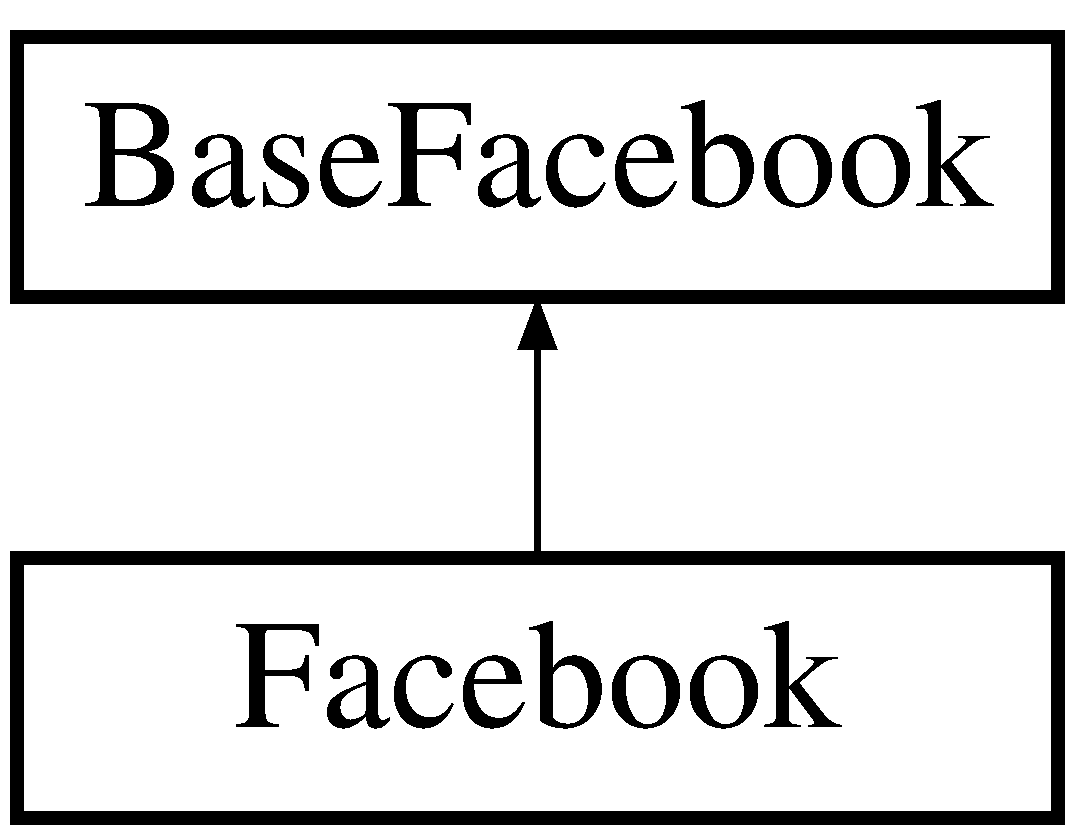
\includegraphics[height=2.000000cm]{class_base_facebook}
\end{center}
\end{figure}
\subsection*{Public Member Functions}
\begin{DoxyCompactItemize}
\item 
\hyperlink{class_base_facebook_af8ca4863484827e521f5052f5dfed642}{\-\_\-\-\_\-construct} (\$config)
\item 
\hyperlink{class_base_facebook_a4691675e86f0fdba08118a0a50d16999}{set\-App\-Id} (\$app\-Id)
\item 
\hyperlink{class_base_facebook_a1a3ad028a497dede716cb101f779a15c}{get\-App\-Id} ()
\item 
\hyperlink{class_base_facebook_afafa43cb0a481b084ae523a04e816016}{set\-Api\-Secret} (\$api\-Secret)
\item 
\hyperlink{class_base_facebook_ac25a51d73a78e3d3308523fc03c93a05}{set\-App\-Secret} (\$app\-Secret)
\item 
\hyperlink{class_base_facebook_ab97bde45113f0c14d1c42c154e39ecf5}{get\-Api\-Secret} ()
\item 
\hyperlink{class_base_facebook_ae53e6a3cfd3b6ca1dba5c1f5568720ec}{get\-App\-Secret} ()
\item 
\hyperlink{class_base_facebook_a9cd44296e92bd602f54c26d613decefc}{set\-File\-Upload\-Support} (\$file\-Upload\-Support)
\item 
\hyperlink{class_base_facebook_a339321887bccd3b1ebc79c433ed97409}{get\-File\-Upload\-Support} ()
\item 
\hyperlink{class_base_facebook_a21f5271bcb490f3c415923ce956d61ad}{use\-File\-Upload\-Support} ()
\item 
\hyperlink{class_base_facebook_a3844fd3db938af8c4d37ed1edeea3ed5}{set\-Access\-Token} (\$access\-\_\-token)
\item 
\hyperlink{class_base_facebook_a1cdac89b20b87c2c2a20137e5e7a8f17}{get\-Access\-Token} ()
\item 
\hyperlink{class_base_facebook_adf3c753e09842db169309daf8713d17a}{get\-Signed\-Request} ()
\item 
\hyperlink{class_base_facebook_a8a3ed9483d09400ec486232401189cba}{get\-User} ()
\item 
\hyperlink{class_base_facebook_ad8f74c26c7a9bcb82dfe3a411419b553}{get\-Login\-Url} (\$params=array())
\item 
\hyperlink{class_base_facebook_a8083255cc3de8af470925baebccffae2}{get\-Logout\-Url} (\$params=array())
\item 
\hyperlink{class_base_facebook_a3ac3ec2796290a2e3e4d511bbe76abee}{get\-Login\-Status\-Url} (\$params=array())
\item 
\hyperlink{class_base_facebook_a22d6a4c1b6dec331c3bc3f7af02849f5}{api} ()
\item 
\hyperlink{class_base_facebook_a4235356d20fcc14a74c1073b59948b65}{destroy\-Session} ()
\end{DoxyCompactItemize}
\subsection*{Public Attributes}
\begin{DoxyCompactItemize}
\item 
const \hyperlink{class_base_facebook_ae0ee825ecd33e197a890c9b47ee14bd8}{V\-E\-R\-S\-I\-O\-N} = '3.\-1.\-1'
\end{DoxyCompactItemize}
\subsection*{Static Public Attributes}
\begin{DoxyCompactItemize}
\item 
static \hyperlink{class_base_facebook_ad48ad58bc8120acf03f199bb100be6dd}{\$\-C\-U\-R\-L\-\_\-\-O\-P\-T\-S}
\item 
static \hyperlink{class_base_facebook_a154dee18518e85547854c5d51f77e314}{\$\-D\-O\-M\-A\-I\-N\-\_\-\-M\-A\-P}
\end{DoxyCompactItemize}
\subsection*{Protected Member Functions}
\begin{DoxyCompactItemize}
\item 
\hyperlink{class_base_facebook_afe9aab209768e4d4cc4c959f4dff4310}{get\-User\-Access\-Token} ()
\item 
\hyperlink{class_base_facebook_ad3dbf5723aa966c9618d1d109526dc4b}{get\-User\-From\-Available\-Data} ()
\item 
\hyperlink{class_base_facebook_a67b1b4b1b2337a342ed03aa0a8f91ec5}{get\-Signed\-Request\-Cookie\-Name} ()
\item 
\hyperlink{class_base_facebook_ac73bdb41c831a2176eaea8902fdb7d71}{get\-Metadata\-Cookie\-Name} ()
\item 
\hyperlink{class_base_facebook_a63452f26d5a4fc7fbcb1732920c1758e}{get\-Code} ()
\item 
\hyperlink{class_base_facebook_ac67c523b16b29ab94354fd518b4daf06}{get\-User\-From\-Access\-Token} ()
\item 
\hyperlink{class_base_facebook_a18b991618948872f3f350ee088fea74d}{get\-Application\-Access\-Token} ()
\item 
\hyperlink{class_base_facebook_a461a0bb17c1aec841d401983e069f06a}{establish\-C\-S\-R\-F\-Token\-State} ()
\item 
\hyperlink{class_base_facebook_a5cf64ed0104ccf5267e9cee1e73ed783}{get\-Access\-Token\-From\-Code} (\$code, \$redirect\-\_\-uri=null)
\item 
\hyperlink{class_base_facebook_a3235e3e5d0c4129e919ab2be464fab4e}{\-\_\-restserver} (\$params)
\item 
\hyperlink{class_base_facebook_a59ec8025b618af99293ac5efc9d88a59}{is\-Video\-Post} (\$path, \$method= 'G\-E\-T')
\item 
\hyperlink{class_base_facebook_af0966973d145fbb9c2add330a46c7587}{\-\_\-graph} (\$path, \$method= 'G\-E\-T', \$params=array())
\item 
\hyperlink{class_base_facebook_a87925b6d625110ec3aab4bad3100d4d3}{\-\_\-oauth\-Request} (\$url, \$params)
\item 
\hyperlink{class_base_facebook_acded7c1ecb37c2745c734f4736b3c8ac}{make\-Request} (\$url, \$params, \$ch=null)
\item 
\hyperlink{class_base_facebook_a0f155bb002187e66febf73bef11aeb4d}{parse\-Signed\-Request} (\$signed\-\_\-request)
\item 
\hyperlink{class_base_facebook_a3a844e7cce1bad59e59b7ebdb93baa8a}{get\-Api\-Url} (\$method)
\item 
\hyperlink{class_base_facebook_a40ca413355e37b68c3649839769bda2b}{get\-Url} (\$name, \$path='', \$params=array())
\item 
\hyperlink{class_base_facebook_a5746a277eddefc701ad5308285252465}{get\-Current\-Url} ()
\item 
\hyperlink{class_base_facebook_a47e7827a14b19657e2a760afa5324dad}{should\-Retain\-Param} (\$param)
\item 
\hyperlink{class_base_facebook_a83875df5a95a05bbbb4857460e743404}{throw\-A\-P\-I\-Exception} (\$result)
\item 
\hyperlink{class_base_facebook_a934183edea46236610bc661c92747c71}{get\-Metadata\-Cookie} ()
\item 
\hyperlink{class_base_facebook_a26198ff065bea23f358854facbafa7db}{set\-Persistent\-Data} (\$key, \$value)
\item 
\hyperlink{class_base_facebook_ad383ccec6f7433c2ab9bb50550df2ce6}{get\-Persistent\-Data} (\$key, \$default=false)
\item 
\hyperlink{class_base_facebook_a3bfb6ef7b1abbd3ec0545be109d32bef}{clear\-Persistent\-Data} (\$key)
\item 
\hyperlink{class_base_facebook_a2f98dbe9b9b63d3e76ba7f1971d80c91}{clear\-All\-Persistent\-Data} ()
\end{DoxyCompactItemize}
\subsection*{Static Protected Member Functions}
\begin{DoxyCompactItemize}
\item 
static \hyperlink{class_base_facebook_a8f2b4289828f4f1e758c05f483eca682}{error\-Log} (\$msg)
\item 
static \hyperlink{class_base_facebook_a8cb499f186fbbd10b7d30c37094d9b97}{base64\-Url\-Decode} (\$input)
\end{DoxyCompactItemize}
\subsection*{Protected Attributes}
\begin{DoxyCompactItemize}
\item 
\hyperlink{class_base_facebook_a90c6ec44757d540ffe1539f512af7469}{\$signed\-Request}
\item 
\hyperlink{class_base_facebook_a8c3903cc0e9a12c87dfae721648491a2}{\$state}
\end{DoxyCompactItemize}
\subsection*{Static Protected Attributes}
\begin{DoxyCompactItemize}
\item 
static \hyperlink{class_base_facebook_a463779b23fc993650d18af395979501d}{\$\-D\-R\-O\-P\-\_\-\-Q\-U\-E\-R\-Y\-\_\-\-P\-A\-R\-A\-M\-S}
\end{DoxyCompactItemize}


\subsection{Detailed Description}
Provides access to the \hyperlink{class_facebook}{Facebook} Platform. This class provides a majority of the functionality needed, but the class is abstract because it is designed to be sub-\/classed. The subclass must implement the four abstract methods listed at the bottom of the file.

\begin{DoxyAuthor}{Author}
Naitik Shah \href{mailto:naitik@facebook.com}{\tt naitik@facebook.\-com} 
\end{DoxyAuthor}


\subsection{Constructor \& Destructor Documentation}
\hypertarget{class_base_facebook_af8ca4863484827e521f5052f5dfed642}{\index{Base\-Facebook@{Base\-Facebook}!\-\_\-\-\_\-construct@{\-\_\-\-\_\-construct}}
\index{\-\_\-\-\_\-construct@{\-\_\-\-\_\-construct}!BaseFacebook@{Base\-Facebook}}
\subsubsection[{\-\_\-\-\_\-construct}]{\setlength{\rightskip}{0pt plus 5cm}Base\-Facebook\-::\-\_\-\-\_\-construct (
\begin{DoxyParamCaption}
\item[{}]{\$config}
\end{DoxyParamCaption}
)}}\label{class_base_facebook_af8ca4863484827e521f5052f5dfed642}
Initialize a \hyperlink{class_facebook}{Facebook} Application.

The configuration\-:
\begin{DoxyItemize}
\item app\-Id\-: the application I\-D
\item secret\-: the application secret
\item file\-Upload\-: (optional) boolean indicating if file uploads are enabled
\end{DoxyItemize}


\begin{DoxyParams}[1]{Parameters}
array & {\em \$config} & The application configuration \\
\hline
\end{DoxyParams}


\subsection{Member Function Documentation}
\hypertarget{class_base_facebook_af0966973d145fbb9c2add330a46c7587}{\index{Base\-Facebook@{Base\-Facebook}!\-\_\-graph@{\-\_\-graph}}
\index{\-\_\-graph@{\-\_\-graph}!BaseFacebook@{Base\-Facebook}}
\subsubsection[{\-\_\-graph}]{\setlength{\rightskip}{0pt plus 5cm}Base\-Facebook\-::\-\_\-graph (
\begin{DoxyParamCaption}
\item[{}]{\$path, }
\item[{}]{\$method = {\ttfamily 'GET'}, }
\item[{}]{\$params = {\ttfamily array()}}
\end{DoxyParamCaption}
)\hspace{0.3cm}{\ttfamily [protected]}}}\label{class_base_facebook_af0966973d145fbb9c2add330a46c7587}
Invoke the Graph A\-P\-I.


\begin{DoxyParams}[1]{Parameters}
string & {\em \$path} & The path (required) \\
\hline
string & {\em \$method} & The http method (default 'G\-E\-T') \\
\hline
array & {\em \$params} & The query/post data\\
\hline
\end{DoxyParams}
\begin{DoxyReturn}{Returns}
mixed The decoded response object 
\end{DoxyReturn}

\begin{DoxyExceptions}{Exceptions}
{\em \hyperlink{class_facebook_api_exception}{Facebook\-Api\-Exception}} & \\
\hline
\end{DoxyExceptions}
\hypertarget{class_base_facebook_a87925b6d625110ec3aab4bad3100d4d3}{\index{Base\-Facebook@{Base\-Facebook}!\-\_\-oauth\-Request@{\-\_\-oauth\-Request}}
\index{\-\_\-oauth\-Request@{\-\_\-oauth\-Request}!BaseFacebook@{Base\-Facebook}}
\subsubsection[{\-\_\-oauth\-Request}]{\setlength{\rightskip}{0pt plus 5cm}Base\-Facebook\-::\-\_\-oauth\-Request (
\begin{DoxyParamCaption}
\item[{}]{\$url, }
\item[{}]{\$params}
\end{DoxyParamCaption}
)\hspace{0.3cm}{\ttfamily [protected]}}}\label{class_base_facebook_a87925b6d625110ec3aab4bad3100d4d3}
Make a O\-Auth \hyperlink{class_request}{Request}.


\begin{DoxyParams}[1]{Parameters}
string & {\em \$url} & The path (required) \\
\hline
array & {\em \$params} & The query/post data\\
\hline
\end{DoxyParams}
\begin{DoxyReturn}{Returns}
string The decoded response object 
\end{DoxyReturn}

\begin{DoxyExceptions}{Exceptions}
{\em \hyperlink{class_facebook_api_exception}{Facebook\-Api\-Exception}} & \\
\hline
\end{DoxyExceptions}
\hypertarget{class_base_facebook_a3235e3e5d0c4129e919ab2be464fab4e}{\index{Base\-Facebook@{Base\-Facebook}!\-\_\-restserver@{\-\_\-restserver}}
\index{\-\_\-restserver@{\-\_\-restserver}!BaseFacebook@{Base\-Facebook}}
\subsubsection[{\-\_\-restserver}]{\setlength{\rightskip}{0pt plus 5cm}Base\-Facebook\-::\-\_\-restserver (
\begin{DoxyParamCaption}
\item[{}]{\$params}
\end{DoxyParamCaption}
)\hspace{0.3cm}{\ttfamily [protected]}}}\label{class_base_facebook_a3235e3e5d0c4129e919ab2be464fab4e}
Invoke the old restserver.\-php endpoint.


\begin{DoxyParams}[1]{Parameters}
array & {\em \$params} & Method call object\\
\hline
\end{DoxyParams}
\begin{DoxyReturn}{Returns}
mixed The decoded response object 
\end{DoxyReturn}

\begin{DoxyExceptions}{Exceptions}
{\em \hyperlink{class_facebook_api_exception}{Facebook\-Api\-Exception}} & \\
\hline
\end{DoxyExceptions}
\hypertarget{class_base_facebook_a22d6a4c1b6dec331c3bc3f7af02849f5}{\index{Base\-Facebook@{Base\-Facebook}!api@{api}}
\index{api@{api}!BaseFacebook@{Base\-Facebook}}
\subsubsection[{api}]{\setlength{\rightskip}{0pt plus 5cm}Base\-Facebook\-::api (
\begin{DoxyParamCaption}
{}
\end{DoxyParamCaption}
)}}\label{class_base_facebook_a22d6a4c1b6dec331c3bc3f7af02849f5}
Make an A\-P\-I call.

\begin{DoxyReturn}{Returns}
mixed The decoded response 
\end{DoxyReturn}
\hypertarget{class_base_facebook_a8cb499f186fbbd10b7d30c37094d9b97}{\index{Base\-Facebook@{Base\-Facebook}!base64\-Url\-Decode@{base64\-Url\-Decode}}
\index{base64\-Url\-Decode@{base64\-Url\-Decode}!BaseFacebook@{Base\-Facebook}}
\subsubsection[{base64\-Url\-Decode}]{\setlength{\rightskip}{0pt plus 5cm}static Base\-Facebook\-::base64\-Url\-Decode (
\begin{DoxyParamCaption}
\item[{}]{\$input}
\end{DoxyParamCaption}
)\hspace{0.3cm}{\ttfamily [static]}, {\ttfamily [protected]}}}\label{class_base_facebook_a8cb499f186fbbd10b7d30c37094d9b97}
Base64 encoding that doesn't need to be urlencode()ed. Exactly the same as base64\-\_\-encode except it uses
\begin{DoxyItemize}
\item instead of + \-\_\- instead of /
\end{DoxyItemize}


\begin{DoxyParams}[1]{Parameters}
string & {\em \$input} & base64\-Url\-Encoded string \\
\hline
\end{DoxyParams}
\begin{DoxyReturn}{Returns}
string 
\end{DoxyReturn}
\hypertarget{class_base_facebook_a2f98dbe9b9b63d3e76ba7f1971d80c91}{\index{Base\-Facebook@{Base\-Facebook}!clear\-All\-Persistent\-Data@{clear\-All\-Persistent\-Data}}
\index{clear\-All\-Persistent\-Data@{clear\-All\-Persistent\-Data}!BaseFacebook@{Base\-Facebook}}
\subsubsection[{clear\-All\-Persistent\-Data}]{\setlength{\rightskip}{0pt plus 5cm}Base\-Facebook\-::clear\-All\-Persistent\-Data (
\begin{DoxyParamCaption}
{}
\end{DoxyParamCaption}
)\hspace{0.3cm}{\ttfamily [abstract]}, {\ttfamily [protected]}}}\label{class_base_facebook_a2f98dbe9b9b63d3e76ba7f1971d80c91}
Clear all data from the persistent storage

\begin{DoxyReturn}{Returns}
void 
\end{DoxyReturn}
\hypertarget{class_base_facebook_a3bfb6ef7b1abbd3ec0545be109d32bef}{\index{Base\-Facebook@{Base\-Facebook}!clear\-Persistent\-Data@{clear\-Persistent\-Data}}
\index{clear\-Persistent\-Data@{clear\-Persistent\-Data}!BaseFacebook@{Base\-Facebook}}
\subsubsection[{clear\-Persistent\-Data}]{\setlength{\rightskip}{0pt plus 5cm}Base\-Facebook\-::clear\-Persistent\-Data (
\begin{DoxyParamCaption}
\item[{}]{\$key}
\end{DoxyParamCaption}
)\hspace{0.3cm}{\ttfamily [abstract]}, {\ttfamily [protected]}}}\label{class_base_facebook_a3bfb6ef7b1abbd3ec0545be109d32bef}
Clear the data with \$key from the persistent storage


\begin{DoxyParams}[1]{Parameters}
string & {\em \$key} & \\
\hline
\end{DoxyParams}
\begin{DoxyReturn}{Returns}
void 
\end{DoxyReturn}
\hypertarget{class_base_facebook_a4235356d20fcc14a74c1073b59948b65}{\index{Base\-Facebook@{Base\-Facebook}!destroy\-Session@{destroy\-Session}}
\index{destroy\-Session@{destroy\-Session}!BaseFacebook@{Base\-Facebook}}
\subsubsection[{destroy\-Session}]{\setlength{\rightskip}{0pt plus 5cm}Base\-Facebook\-::destroy\-Session (
\begin{DoxyParamCaption}
{}
\end{DoxyParamCaption}
)}}\label{class_base_facebook_a4235356d20fcc14a74c1073b59948b65}
Destroy the current session \hypertarget{class_base_facebook_a8f2b4289828f4f1e758c05f483eca682}{\index{Base\-Facebook@{Base\-Facebook}!error\-Log@{error\-Log}}
\index{error\-Log@{error\-Log}!BaseFacebook@{Base\-Facebook}}
\subsubsection[{error\-Log}]{\setlength{\rightskip}{0pt plus 5cm}static Base\-Facebook\-::error\-Log (
\begin{DoxyParamCaption}
\item[{}]{\$msg}
\end{DoxyParamCaption}
)\hspace{0.3cm}{\ttfamily [static]}, {\ttfamily [protected]}}}\label{class_base_facebook_a8f2b4289828f4f1e758c05f483eca682}
Prints to the error log if you aren't in command line mode.


\begin{DoxyParams}[1]{Parameters}
string & {\em \$msg} & Log message \\
\hline
\end{DoxyParams}
\hypertarget{class_base_facebook_a461a0bb17c1aec841d401983e069f06a}{\index{Base\-Facebook@{Base\-Facebook}!establish\-C\-S\-R\-F\-Token\-State@{establish\-C\-S\-R\-F\-Token\-State}}
\index{establish\-C\-S\-R\-F\-Token\-State@{establish\-C\-S\-R\-F\-Token\-State}!BaseFacebook@{Base\-Facebook}}
\subsubsection[{establish\-C\-S\-R\-F\-Token\-State}]{\setlength{\rightskip}{0pt plus 5cm}Base\-Facebook\-::establish\-C\-S\-R\-F\-Token\-State (
\begin{DoxyParamCaption}
{}
\end{DoxyParamCaption}
)\hspace{0.3cm}{\ttfamily [protected]}}}\label{class_base_facebook_a461a0bb17c1aec841d401983e069f06a}
Lays down a C\-S\-R\-F state token for this process.

\begin{DoxyReturn}{Returns}
void 
\end{DoxyReturn}
\hypertarget{class_base_facebook_a1cdac89b20b87c2c2a20137e5e7a8f17}{\index{Base\-Facebook@{Base\-Facebook}!get\-Access\-Token@{get\-Access\-Token}}
\index{get\-Access\-Token@{get\-Access\-Token}!BaseFacebook@{Base\-Facebook}}
\subsubsection[{get\-Access\-Token}]{\setlength{\rightskip}{0pt plus 5cm}Base\-Facebook\-::get\-Access\-Token (
\begin{DoxyParamCaption}
{}
\end{DoxyParamCaption}
)}}\label{class_base_facebook_a1cdac89b20b87c2c2a20137e5e7a8f17}
Determines the access token that should be used for A\-P\-I calls. The first time this is called, \$this-\/$>$access\-Token is set equal to either a valid user access token, or it's set to the application access token if a valid user access token wasn't available. Subsequent calls return whatever the first call returned.

\begin{DoxyReturn}{Returns}
string The access token 
\end{DoxyReturn}
\hypertarget{class_base_facebook_a5cf64ed0104ccf5267e9cee1e73ed783}{\index{Base\-Facebook@{Base\-Facebook}!get\-Access\-Token\-From\-Code@{get\-Access\-Token\-From\-Code}}
\index{get\-Access\-Token\-From\-Code@{get\-Access\-Token\-From\-Code}!BaseFacebook@{Base\-Facebook}}
\subsubsection[{get\-Access\-Token\-From\-Code}]{\setlength{\rightskip}{0pt plus 5cm}Base\-Facebook\-::get\-Access\-Token\-From\-Code (
\begin{DoxyParamCaption}
\item[{}]{\$code, }
\item[{}]{\$redirect\-\_\-uri = {\ttfamily null}}
\end{DoxyParamCaption}
)\hspace{0.3cm}{\ttfamily [protected]}}}\label{class_base_facebook_a5cf64ed0104ccf5267e9cee1e73ed783}
Retrieves an access token for the given authorization code (previously generated from www.\-facebook.\-com on behalf of a specific user). The authorization code is sent to graph.\-facebook.\-com and a legitimate access token is generated provided the access token and the user for which it was generated all match, and the user is either logged in to \hyperlink{class_facebook}{Facebook} or has granted an offline access permission.


\begin{DoxyParams}[1]{Parameters}
string & {\em \$code} & An authorization code. \\
\hline
\end{DoxyParams}
\begin{DoxyReturn}{Returns}
mixed An access token exchanged for the authorization code, or false if an access token could not be generated. 
\end{DoxyReturn}
\hypertarget{class_base_facebook_ab97bde45113f0c14d1c42c154e39ecf5}{\index{Base\-Facebook@{Base\-Facebook}!get\-Api\-Secret@{get\-Api\-Secret}}
\index{get\-Api\-Secret@{get\-Api\-Secret}!BaseFacebook@{Base\-Facebook}}
\subsubsection[{get\-Api\-Secret}]{\setlength{\rightskip}{0pt plus 5cm}Base\-Facebook\-::get\-Api\-Secret (
\begin{DoxyParamCaption}
{}
\end{DoxyParamCaption}
)}}\label{class_base_facebook_ab97bde45113f0c14d1c42c154e39ecf5}
Get the App Secret.

\begin{DoxyReturn}{Returns}
string the App Secret 
\end{DoxyReturn}
\begin{DoxyRefDesc}{Deprecated}
\item[\hyperlink{deprecated__deprecated000002}{Deprecated}]\end{DoxyRefDesc}
\hypertarget{class_base_facebook_a3a844e7cce1bad59e59b7ebdb93baa8a}{\index{Base\-Facebook@{Base\-Facebook}!get\-Api\-Url@{get\-Api\-Url}}
\index{get\-Api\-Url@{get\-Api\-Url}!BaseFacebook@{Base\-Facebook}}
\subsubsection[{get\-Api\-Url}]{\setlength{\rightskip}{0pt plus 5cm}Base\-Facebook\-::get\-Api\-Url (
\begin{DoxyParamCaption}
\item[{}]{\$method}
\end{DoxyParamCaption}
)\hspace{0.3cm}{\ttfamily [protected]}}}\label{class_base_facebook_a3a844e7cce1bad59e59b7ebdb93baa8a}
Build the U\-R\-L for api given parameters.


\begin{DoxyParams}{Parameters}
{\em \$method} & String the method name. \\
\hline
\end{DoxyParams}
\begin{DoxyReturn}{Returns}
string The U\-R\-L for the given parameters 
\end{DoxyReturn}
\hypertarget{class_base_facebook_a1a3ad028a497dede716cb101f779a15c}{\index{Base\-Facebook@{Base\-Facebook}!get\-App\-Id@{get\-App\-Id}}
\index{get\-App\-Id@{get\-App\-Id}!BaseFacebook@{Base\-Facebook}}
\subsubsection[{get\-App\-Id}]{\setlength{\rightskip}{0pt plus 5cm}Base\-Facebook\-::get\-App\-Id (
\begin{DoxyParamCaption}
{}
\end{DoxyParamCaption}
)}}\label{class_base_facebook_a1a3ad028a497dede716cb101f779a15c}
Get the Application I\-D.

\begin{DoxyReturn}{Returns}
string the Application I\-D 
\end{DoxyReturn}
\hypertarget{class_base_facebook_a18b991618948872f3f350ee088fea74d}{\index{Base\-Facebook@{Base\-Facebook}!get\-Application\-Access\-Token@{get\-Application\-Access\-Token}}
\index{get\-Application\-Access\-Token@{get\-Application\-Access\-Token}!BaseFacebook@{Base\-Facebook}}
\subsubsection[{get\-Application\-Access\-Token}]{\setlength{\rightskip}{0pt plus 5cm}Base\-Facebook\-::get\-Application\-Access\-Token (
\begin{DoxyParamCaption}
{}
\end{DoxyParamCaption}
)\hspace{0.3cm}{\ttfamily [protected]}}}\label{class_base_facebook_a18b991618948872f3f350ee088fea74d}
Returns the access token that should be used for logged out users when no authorization code is available.

\begin{DoxyReturn}{Returns}
string The application access token, useful for gathering public information about users and applications. 
\end{DoxyReturn}
\hypertarget{class_base_facebook_ae53e6a3cfd3b6ca1dba5c1f5568720ec}{\index{Base\-Facebook@{Base\-Facebook}!get\-App\-Secret@{get\-App\-Secret}}
\index{get\-App\-Secret@{get\-App\-Secret}!BaseFacebook@{Base\-Facebook}}
\subsubsection[{get\-App\-Secret}]{\setlength{\rightskip}{0pt plus 5cm}Base\-Facebook\-::get\-App\-Secret (
\begin{DoxyParamCaption}
{}
\end{DoxyParamCaption}
)}}\label{class_base_facebook_ae53e6a3cfd3b6ca1dba5c1f5568720ec}
Get the App Secret.

\begin{DoxyReturn}{Returns}
string the App Secret 
\end{DoxyReturn}
\hypertarget{class_base_facebook_a63452f26d5a4fc7fbcb1732920c1758e}{\index{Base\-Facebook@{Base\-Facebook}!get\-Code@{get\-Code}}
\index{get\-Code@{get\-Code}!BaseFacebook@{Base\-Facebook}}
\subsubsection[{get\-Code}]{\setlength{\rightskip}{0pt plus 5cm}Base\-Facebook\-::get\-Code (
\begin{DoxyParamCaption}
{}
\end{DoxyParamCaption}
)\hspace{0.3cm}{\ttfamily [protected]}}}\label{class_base_facebook_a63452f26d5a4fc7fbcb1732920c1758e}
Get the authorization code from the query parameters, if it exists, and otherwise return false to signal no authorization code was discoverable.

\begin{DoxyReturn}{Returns}
mixed The authorization code, or false if the authorization code could not be determined. 
\end{DoxyReturn}
\hypertarget{class_base_facebook_a5746a277eddefc701ad5308285252465}{\index{Base\-Facebook@{Base\-Facebook}!get\-Current\-Url@{get\-Current\-Url}}
\index{get\-Current\-Url@{get\-Current\-Url}!BaseFacebook@{Base\-Facebook}}
\subsubsection[{get\-Current\-Url}]{\setlength{\rightskip}{0pt plus 5cm}Base\-Facebook\-::get\-Current\-Url (
\begin{DoxyParamCaption}
{}
\end{DoxyParamCaption}
)\hspace{0.3cm}{\ttfamily [protected]}}}\label{class_base_facebook_a5746a277eddefc701ad5308285252465}
Returns the Current U\-R\-L, stripping it of known F\-B parameters that should not persist.

\begin{DoxyReturn}{Returns}
string The current U\-R\-L 
\end{DoxyReturn}
\hypertarget{class_base_facebook_a339321887bccd3b1ebc79c433ed97409}{\index{Base\-Facebook@{Base\-Facebook}!get\-File\-Upload\-Support@{get\-File\-Upload\-Support}}
\index{get\-File\-Upload\-Support@{get\-File\-Upload\-Support}!BaseFacebook@{Base\-Facebook}}
\subsubsection[{get\-File\-Upload\-Support}]{\setlength{\rightskip}{0pt plus 5cm}Base\-Facebook\-::get\-File\-Upload\-Support (
\begin{DoxyParamCaption}
{}
\end{DoxyParamCaption}
)}}\label{class_base_facebook_a339321887bccd3b1ebc79c433ed97409}
Get the file upload support status.

\begin{DoxyReturn}{Returns}
boolean true if and only if the server supports file upload. 
\end{DoxyReturn}
\hypertarget{class_base_facebook_a3ac3ec2796290a2e3e4d511bbe76abee}{\index{Base\-Facebook@{Base\-Facebook}!get\-Login\-Status\-Url@{get\-Login\-Status\-Url}}
\index{get\-Login\-Status\-Url@{get\-Login\-Status\-Url}!BaseFacebook@{Base\-Facebook}}
\subsubsection[{get\-Login\-Status\-Url}]{\setlength{\rightskip}{0pt plus 5cm}Base\-Facebook\-::get\-Login\-Status\-Url (
\begin{DoxyParamCaption}
\item[{}]{\$params = {\ttfamily array()}}
\end{DoxyParamCaption}
)}}\label{class_base_facebook_a3ac3ec2796290a2e3e4d511bbe76abee}
Get a login status U\-R\-L to fetch the status from \hyperlink{class_facebook}{Facebook}.

The parameters\-:
\begin{DoxyItemize}
\item ok\-\_\-session\-: the U\-R\-L to go to if a session is found
\item no\-\_\-session\-: the U\-R\-L to go to if the user is not connected
\item no\-\_\-user\-: the U\-R\-L to go to if the user is not signed into facebook
\end{DoxyItemize}


\begin{DoxyParams}[1]{Parameters}
array & {\em \$params} & Provide custom parameters \\
\hline
\end{DoxyParams}
\begin{DoxyReturn}{Returns}
string The U\-R\-L for the logout flow 
\end{DoxyReturn}
\hypertarget{class_base_facebook_ad8f74c26c7a9bcb82dfe3a411419b553}{\index{Base\-Facebook@{Base\-Facebook}!get\-Login\-Url@{get\-Login\-Url}}
\index{get\-Login\-Url@{get\-Login\-Url}!BaseFacebook@{Base\-Facebook}}
\subsubsection[{get\-Login\-Url}]{\setlength{\rightskip}{0pt plus 5cm}Base\-Facebook\-::get\-Login\-Url (
\begin{DoxyParamCaption}
\item[{}]{\$params = {\ttfamily array()}}
\end{DoxyParamCaption}
)}}\label{class_base_facebook_ad8f74c26c7a9bcb82dfe3a411419b553}
Get a Login U\-R\-L for use with redirects. By default, full page redirect is assumed. If you are using the generated U\-R\-L with a window.\-open() call in Java\-Script, you can pass in display=popup as part of the \$params.

The parameters\-:
\begin{DoxyItemize}
\item redirect\-\_\-uri\-: the url to go to after a successful login
\item scope\-: comma separated list of requested extended perms
\end{DoxyItemize}


\begin{DoxyParams}[1]{Parameters}
array & {\em \$params} & Provide custom parameters \\
\hline
\end{DoxyParams}
\begin{DoxyReturn}{Returns}
string The U\-R\-L for the login flow 
\end{DoxyReturn}
\hypertarget{class_base_facebook_a8083255cc3de8af470925baebccffae2}{\index{Base\-Facebook@{Base\-Facebook}!get\-Logout\-Url@{get\-Logout\-Url}}
\index{get\-Logout\-Url@{get\-Logout\-Url}!BaseFacebook@{Base\-Facebook}}
\subsubsection[{get\-Logout\-Url}]{\setlength{\rightskip}{0pt plus 5cm}Base\-Facebook\-::get\-Logout\-Url (
\begin{DoxyParamCaption}
\item[{}]{\$params = {\ttfamily array()}}
\end{DoxyParamCaption}
)}}\label{class_base_facebook_a8083255cc3de8af470925baebccffae2}
Get a Logout U\-R\-L suitable for use with redirects.

The parameters\-:
\begin{DoxyItemize}
\item next\-: the url to go to after a successful logout
\end{DoxyItemize}


\begin{DoxyParams}[1]{Parameters}
array & {\em \$params} & Provide custom parameters \\
\hline
\end{DoxyParams}
\begin{DoxyReturn}{Returns}
string The U\-R\-L for the logout flow 
\end{DoxyReturn}
\hypertarget{class_base_facebook_a934183edea46236610bc661c92747c71}{\index{Base\-Facebook@{Base\-Facebook}!get\-Metadata\-Cookie@{get\-Metadata\-Cookie}}
\index{get\-Metadata\-Cookie@{get\-Metadata\-Cookie}!BaseFacebook@{Base\-Facebook}}
\subsubsection[{get\-Metadata\-Cookie}]{\setlength{\rightskip}{0pt plus 5cm}Base\-Facebook\-::get\-Metadata\-Cookie (
\begin{DoxyParamCaption}
{}
\end{DoxyParamCaption}
)\hspace{0.3cm}{\ttfamily [protected]}}}\label{class_base_facebook_a934183edea46236610bc661c92747c71}
Parses the metadata cookie that our Javascript A\-P\-I set

\begin{DoxyReturn}{Returns}
an array mapping key to value 
\end{DoxyReturn}
\hypertarget{class_base_facebook_ac73bdb41c831a2176eaea8902fdb7d71}{\index{Base\-Facebook@{Base\-Facebook}!get\-Metadata\-Cookie\-Name@{get\-Metadata\-Cookie\-Name}}
\index{get\-Metadata\-Cookie\-Name@{get\-Metadata\-Cookie\-Name}!BaseFacebook@{Base\-Facebook}}
\subsubsection[{get\-Metadata\-Cookie\-Name}]{\setlength{\rightskip}{0pt plus 5cm}Base\-Facebook\-::get\-Metadata\-Cookie\-Name (
\begin{DoxyParamCaption}
{}
\end{DoxyParamCaption}
)\hspace{0.3cm}{\ttfamily [protected]}}}\label{class_base_facebook_ac73bdb41c831a2176eaea8902fdb7d71}
Constructs and returns the name of the coookie that potentially contain metadata. The cookie is not set by the \hyperlink{class_base_facebook}{Base\-Facebook} class, but it may be set by the Java\-Script S\-D\-K.

\begin{DoxyReturn}{Returns}
string the name of the cookie that would house metadata. 
\end{DoxyReturn}
\hypertarget{class_base_facebook_ad383ccec6f7433c2ab9bb50550df2ce6}{\index{Base\-Facebook@{Base\-Facebook}!get\-Persistent\-Data@{get\-Persistent\-Data}}
\index{get\-Persistent\-Data@{get\-Persistent\-Data}!BaseFacebook@{Base\-Facebook}}
\subsubsection[{get\-Persistent\-Data}]{\setlength{\rightskip}{0pt plus 5cm}Base\-Facebook\-::get\-Persistent\-Data (
\begin{DoxyParamCaption}
\item[{}]{\$key, }
\item[{}]{\$default = {\ttfamily false}}
\end{DoxyParamCaption}
)\hspace{0.3cm}{\ttfamily [abstract]}, {\ttfamily [protected]}}}\label{class_base_facebook_ad383ccec6f7433c2ab9bb50550df2ce6}
Get the data for \$key, persisted by \hyperlink{class_base_facebook_a26198ff065bea23f358854facbafa7db}{Base\-Facebook\-::set\-Persistent\-Data()}


\begin{DoxyParams}[1]{Parameters}
string & {\em \$key} & The key of the data to retrieve \\
\hline
boolean & {\em \$default} & The default value to return if \$key is not found\\
\hline
\end{DoxyParams}
\begin{DoxyReturn}{Returns}
mixed 
\end{DoxyReturn}
\hypertarget{class_base_facebook_adf3c753e09842db169309daf8713d17a}{\index{Base\-Facebook@{Base\-Facebook}!get\-Signed\-Request@{get\-Signed\-Request}}
\index{get\-Signed\-Request@{get\-Signed\-Request}!BaseFacebook@{Base\-Facebook}}
\subsubsection[{get\-Signed\-Request}]{\setlength{\rightskip}{0pt plus 5cm}Base\-Facebook\-::get\-Signed\-Request (
\begin{DoxyParamCaption}
{}
\end{DoxyParamCaption}
)}}\label{class_base_facebook_adf3c753e09842db169309daf8713d17a}
Retrieve the signed request, either from a request parameter or, if not present, from a cookie.

\begin{DoxyReturn}{Returns}
string the signed request, if available, or null otherwise. 
\end{DoxyReturn}
\hypertarget{class_base_facebook_a67b1b4b1b2337a342ed03aa0a8f91ec5}{\index{Base\-Facebook@{Base\-Facebook}!get\-Signed\-Request\-Cookie\-Name@{get\-Signed\-Request\-Cookie\-Name}}
\index{get\-Signed\-Request\-Cookie\-Name@{get\-Signed\-Request\-Cookie\-Name}!BaseFacebook@{Base\-Facebook}}
\subsubsection[{get\-Signed\-Request\-Cookie\-Name}]{\setlength{\rightskip}{0pt plus 5cm}Base\-Facebook\-::get\-Signed\-Request\-Cookie\-Name (
\begin{DoxyParamCaption}
{}
\end{DoxyParamCaption}
)\hspace{0.3cm}{\ttfamily [protected]}}}\label{class_base_facebook_a67b1b4b1b2337a342ed03aa0a8f91ec5}
Constructs and returns the name of the cookie that potentially houses the signed request for the app user. The cookie is not set by the \hyperlink{class_base_facebook}{Base\-Facebook} class, but it may be set by the Java\-Script S\-D\-K.

\begin{DoxyReturn}{Returns}
string the name of the cookie that would house the signed request value. 
\end{DoxyReturn}
\hypertarget{class_base_facebook_a40ca413355e37b68c3649839769bda2b}{\index{Base\-Facebook@{Base\-Facebook}!get\-Url@{get\-Url}}
\index{get\-Url@{get\-Url}!BaseFacebook@{Base\-Facebook}}
\subsubsection[{get\-Url}]{\setlength{\rightskip}{0pt plus 5cm}Base\-Facebook\-::get\-Url (
\begin{DoxyParamCaption}
\item[{}]{\$name, }
\item[{}]{\$path = {\ttfamily ''}, }
\item[{}]{\$params = {\ttfamily array()}}
\end{DoxyParamCaption}
)\hspace{0.3cm}{\ttfamily [protected]}}}\label{class_base_facebook_a40ca413355e37b68c3649839769bda2b}
Build the U\-R\-L for given domain alias, path and parameters.


\begin{DoxyParams}{Parameters}
{\em \$name} & string The name of the domain \\
\hline
{\em \$path} & string Optional path (without a leading slash) \\
\hline
{\em \$params} & array Optional query parameters\\
\hline
\end{DoxyParams}
\begin{DoxyReturn}{Returns}
string The U\-R\-L for the given parameters 
\end{DoxyReturn}
\hypertarget{class_base_facebook_a8a3ed9483d09400ec486232401189cba}{\index{Base\-Facebook@{Base\-Facebook}!get\-User@{get\-User}}
\index{get\-User@{get\-User}!BaseFacebook@{Base\-Facebook}}
\subsubsection[{get\-User}]{\setlength{\rightskip}{0pt plus 5cm}Base\-Facebook\-::get\-User (
\begin{DoxyParamCaption}
{}
\end{DoxyParamCaption}
)}}\label{class_base_facebook_a8a3ed9483d09400ec486232401189cba}
Get the U\-I\-D of the connected user, or 0 if the \hyperlink{class_facebook}{Facebook} user is not connected.

\begin{DoxyReturn}{Returns}
string the U\-I\-D if available. 
\end{DoxyReturn}
\hypertarget{class_base_facebook_afe9aab209768e4d4cc4c959f4dff4310}{\index{Base\-Facebook@{Base\-Facebook}!get\-User\-Access\-Token@{get\-User\-Access\-Token}}
\index{get\-User\-Access\-Token@{get\-User\-Access\-Token}!BaseFacebook@{Base\-Facebook}}
\subsubsection[{get\-User\-Access\-Token}]{\setlength{\rightskip}{0pt plus 5cm}Base\-Facebook\-::get\-User\-Access\-Token (
\begin{DoxyParamCaption}
{}
\end{DoxyParamCaption}
)\hspace{0.3cm}{\ttfamily [protected]}}}\label{class_base_facebook_afe9aab209768e4d4cc4c959f4dff4310}
Determines and returns the user access token, first using the signed request if present, and then falling back on the authorization code if present. The intent is to return a valid user access token, or false if one is determined to not be available.

\begin{DoxyReturn}{Returns}
string A valid user access token, or false if one could not be determined. 
\end{DoxyReturn}
\hypertarget{class_base_facebook_ac67c523b16b29ab94354fd518b4daf06}{\index{Base\-Facebook@{Base\-Facebook}!get\-User\-From\-Access\-Token@{get\-User\-From\-Access\-Token}}
\index{get\-User\-From\-Access\-Token@{get\-User\-From\-Access\-Token}!BaseFacebook@{Base\-Facebook}}
\subsubsection[{get\-User\-From\-Access\-Token}]{\setlength{\rightskip}{0pt plus 5cm}Base\-Facebook\-::get\-User\-From\-Access\-Token (
\begin{DoxyParamCaption}
{}
\end{DoxyParamCaption}
)\hspace{0.3cm}{\ttfamily [protected]}}}\label{class_base_facebook_ac67c523b16b29ab94354fd518b4daf06}
Retrieves the U\-I\-D with the understanding that \$this-\/$>$access\-Token has already been set and is seemingly legitimate. It relies on \hyperlink{class_facebook}{Facebook}'s Graph A\-P\-I to retrieve user information and then extract the user I\-D.

\begin{DoxyReturn}{Returns}
integer Returns the U\-I\-D of the \hyperlink{class_facebook}{Facebook} user, or 0 if the \hyperlink{class_facebook}{Facebook} user could not be determined. 
\end{DoxyReturn}
\hypertarget{class_base_facebook_ad3dbf5723aa966c9618d1d109526dc4b}{\index{Base\-Facebook@{Base\-Facebook}!get\-User\-From\-Available\-Data@{get\-User\-From\-Available\-Data}}
\index{get\-User\-From\-Available\-Data@{get\-User\-From\-Available\-Data}!BaseFacebook@{Base\-Facebook}}
\subsubsection[{get\-User\-From\-Available\-Data}]{\setlength{\rightskip}{0pt plus 5cm}Base\-Facebook\-::get\-User\-From\-Available\-Data (
\begin{DoxyParamCaption}
{}
\end{DoxyParamCaption}
)\hspace{0.3cm}{\ttfamily [protected]}}}\label{class_base_facebook_ad3dbf5723aa966c9618d1d109526dc4b}
Determines the connected user by first examining any signed requests, then considering an authorization code, and then falling back to any persistent store storing the user.

\begin{DoxyReturn}{Returns}
integer The id of the connected \hyperlink{class_facebook}{Facebook} user, or 0 if no such user exists. 
\end{DoxyReturn}
\hypertarget{class_base_facebook_a59ec8025b618af99293ac5efc9d88a59}{\index{Base\-Facebook@{Base\-Facebook}!is\-Video\-Post@{is\-Video\-Post}}
\index{is\-Video\-Post@{is\-Video\-Post}!BaseFacebook@{Base\-Facebook}}
\subsubsection[{is\-Video\-Post}]{\setlength{\rightskip}{0pt plus 5cm}Base\-Facebook\-::is\-Video\-Post (
\begin{DoxyParamCaption}
\item[{}]{\$path, }
\item[{}]{\$method = {\ttfamily 'GET'}}
\end{DoxyParamCaption}
)\hspace{0.3cm}{\ttfamily [protected]}}}\label{class_base_facebook_a59ec8025b618af99293ac5efc9d88a59}
Return true if this is video post.


\begin{DoxyParams}[1]{Parameters}
string & {\em \$path} & The path \\
\hline
string & {\em \$method} & The http method (default 'G\-E\-T')\\
\hline
\end{DoxyParams}
\begin{DoxyReturn}{Returns}
boolean true if this is video post 
\end{DoxyReturn}
\hypertarget{class_base_facebook_acded7c1ecb37c2745c734f4736b3c8ac}{\index{Base\-Facebook@{Base\-Facebook}!make\-Request@{make\-Request}}
\index{make\-Request@{make\-Request}!BaseFacebook@{Base\-Facebook}}
\subsubsection[{make\-Request}]{\setlength{\rightskip}{0pt plus 5cm}Base\-Facebook\-::make\-Request (
\begin{DoxyParamCaption}
\item[{}]{\$url, }
\item[{}]{\$params, }
\item[{}]{\$ch = {\ttfamily null}}
\end{DoxyParamCaption}
)\hspace{0.3cm}{\ttfamily [protected]}}}\label{class_base_facebook_acded7c1ecb37c2745c734f4736b3c8ac}
Makes an H\-T\-T\-P request. This method can be overridden by subclasses if developers want to do fancier things or use something other than curl to make the request.


\begin{DoxyParams}[1]{Parameters}
string & {\em \$url} & The U\-R\-L to make the request to \\
\hline
array & {\em \$params} & The parameters to use for the P\-O\-S\-T body \\
\hline
Curl\-Handler & {\em \$ch} & Initialized curl handle\\
\hline
\end{DoxyParams}
\begin{DoxyReturn}{Returns}
string The response text 
\end{DoxyReturn}
\hypertarget{class_base_facebook_a0f155bb002187e66febf73bef11aeb4d}{\index{Base\-Facebook@{Base\-Facebook}!parse\-Signed\-Request@{parse\-Signed\-Request}}
\index{parse\-Signed\-Request@{parse\-Signed\-Request}!BaseFacebook@{Base\-Facebook}}
\subsubsection[{parse\-Signed\-Request}]{\setlength{\rightskip}{0pt plus 5cm}Base\-Facebook\-::parse\-Signed\-Request (
\begin{DoxyParamCaption}
\item[{}]{\$signed\-\_\-request}
\end{DoxyParamCaption}
)\hspace{0.3cm}{\ttfamily [protected]}}}\label{class_base_facebook_a0f155bb002187e66febf73bef11aeb4d}
Parses a signed\-\_\-request and validates the signature.


\begin{DoxyParams}[1]{Parameters}
string & {\em \$signed\-\_\-request} & A signed token \\
\hline
\end{DoxyParams}
\begin{DoxyReturn}{Returns}
array The payload inside it or null if the sig is wrong 
\end{DoxyReturn}
\hypertarget{class_base_facebook_a3844fd3db938af8c4d37ed1edeea3ed5}{\index{Base\-Facebook@{Base\-Facebook}!set\-Access\-Token@{set\-Access\-Token}}
\index{set\-Access\-Token@{set\-Access\-Token}!BaseFacebook@{Base\-Facebook}}
\subsubsection[{set\-Access\-Token}]{\setlength{\rightskip}{0pt plus 5cm}Base\-Facebook\-::set\-Access\-Token (
\begin{DoxyParamCaption}
\item[{}]{\$access\-\_\-token}
\end{DoxyParamCaption}
)}}\label{class_base_facebook_a3844fd3db938af8c4d37ed1edeea3ed5}
Sets the access token for api calls. Use this if you get your access token by other means and just want the S\-D\-K to use it.


\begin{DoxyParams}[1]{Parameters}
string & {\em \$access\-\_\-token} & an access token. \\
\hline
\end{DoxyParams}
\begin{DoxyReturn}{Returns}
\hyperlink{class_base_facebook}{Base\-Facebook} 
\end{DoxyReturn}
\hypertarget{class_base_facebook_afafa43cb0a481b084ae523a04e816016}{\index{Base\-Facebook@{Base\-Facebook}!set\-Api\-Secret@{set\-Api\-Secret}}
\index{set\-Api\-Secret@{set\-Api\-Secret}!BaseFacebook@{Base\-Facebook}}
\subsubsection[{set\-Api\-Secret}]{\setlength{\rightskip}{0pt plus 5cm}Base\-Facebook\-::set\-Api\-Secret (
\begin{DoxyParamCaption}
\item[{}]{\$api\-Secret}
\end{DoxyParamCaption}
)}}\label{class_base_facebook_afafa43cb0a481b084ae523a04e816016}
Set the App Secret.


\begin{DoxyParams}[1]{Parameters}
string & {\em \$api\-Secret} & The App Secret \\
\hline
\end{DoxyParams}
\begin{DoxyReturn}{Returns}
\hyperlink{class_base_facebook}{Base\-Facebook} 
\end{DoxyReturn}
\begin{DoxyRefDesc}{Deprecated}
\item[\hyperlink{deprecated__deprecated000001}{Deprecated}]\end{DoxyRefDesc}
\hypertarget{class_base_facebook_a4691675e86f0fdba08118a0a50d16999}{\index{Base\-Facebook@{Base\-Facebook}!set\-App\-Id@{set\-App\-Id}}
\index{set\-App\-Id@{set\-App\-Id}!BaseFacebook@{Base\-Facebook}}
\subsubsection[{set\-App\-Id}]{\setlength{\rightskip}{0pt plus 5cm}Base\-Facebook\-::set\-App\-Id (
\begin{DoxyParamCaption}
\item[{}]{\$app\-Id}
\end{DoxyParamCaption}
)}}\label{class_base_facebook_a4691675e86f0fdba08118a0a50d16999}
Set the Application I\-D.


\begin{DoxyParams}[1]{Parameters}
string & {\em \$app\-Id} & The Application I\-D \\
\hline
\end{DoxyParams}
\begin{DoxyReturn}{Returns}
\hyperlink{class_base_facebook}{Base\-Facebook} 
\end{DoxyReturn}
\hypertarget{class_base_facebook_ac25a51d73a78e3d3308523fc03c93a05}{\index{Base\-Facebook@{Base\-Facebook}!set\-App\-Secret@{set\-App\-Secret}}
\index{set\-App\-Secret@{set\-App\-Secret}!BaseFacebook@{Base\-Facebook}}
\subsubsection[{set\-App\-Secret}]{\setlength{\rightskip}{0pt plus 5cm}Base\-Facebook\-::set\-App\-Secret (
\begin{DoxyParamCaption}
\item[{}]{\$app\-Secret}
\end{DoxyParamCaption}
)}}\label{class_base_facebook_ac25a51d73a78e3d3308523fc03c93a05}
Set the App Secret.


\begin{DoxyParams}[1]{Parameters}
string & {\em \$app\-Secret} & The App Secret \\
\hline
\end{DoxyParams}
\begin{DoxyReturn}{Returns}
\hyperlink{class_base_facebook}{Base\-Facebook} 
\end{DoxyReturn}
\hypertarget{class_base_facebook_a9cd44296e92bd602f54c26d613decefc}{\index{Base\-Facebook@{Base\-Facebook}!set\-File\-Upload\-Support@{set\-File\-Upload\-Support}}
\index{set\-File\-Upload\-Support@{set\-File\-Upload\-Support}!BaseFacebook@{Base\-Facebook}}
\subsubsection[{set\-File\-Upload\-Support}]{\setlength{\rightskip}{0pt plus 5cm}Base\-Facebook\-::set\-File\-Upload\-Support (
\begin{DoxyParamCaption}
\item[{}]{\$file\-Upload\-Support}
\end{DoxyParamCaption}
)}}\label{class_base_facebook_a9cd44296e92bd602f54c26d613decefc}
Set the file upload support status.


\begin{DoxyParams}[1]{Parameters}
boolean & {\em \$file\-Upload\-Support} & The file upload support status. \\
\hline
\end{DoxyParams}
\begin{DoxyReturn}{Returns}
\hyperlink{class_base_facebook}{Base\-Facebook} 
\end{DoxyReturn}
\hypertarget{class_base_facebook_a26198ff065bea23f358854facbafa7db}{\index{Base\-Facebook@{Base\-Facebook}!set\-Persistent\-Data@{set\-Persistent\-Data}}
\index{set\-Persistent\-Data@{set\-Persistent\-Data}!BaseFacebook@{Base\-Facebook}}
\subsubsection[{set\-Persistent\-Data}]{\setlength{\rightskip}{0pt plus 5cm}Base\-Facebook\-::set\-Persistent\-Data (
\begin{DoxyParamCaption}
\item[{}]{\$key, }
\item[{}]{\$value}
\end{DoxyParamCaption}
)\hspace{0.3cm}{\ttfamily [abstract]}, {\ttfamily [protected]}}}\label{class_base_facebook_a26198ff065bea23f358854facbafa7db}
Each of the following four methods should be overridden in a concrete subclass, as they are in the provided \hyperlink{class_facebook}{Facebook} class. The \hyperlink{class_facebook}{Facebook} class uses P\-H\-P sessions to provide a primitive persistent store, but another subclass--one that you implement-- might use a database, memcache, or an in-\/memory cache.

\begin{DoxySeeAlso}{See Also}
\hyperlink{class_facebook}{Facebook} Stores the given (\$key, \$value) pair, so that future calls to \hyperlink{class_base_facebook_ad383ccec6f7433c2ab9bb50550df2ce6}{get\-Persistent\-Data}(\$key) return \$value. This call may be in another request.
\end{DoxySeeAlso}

\begin{DoxyParams}[1]{Parameters}
string & {\em \$key} & \\
\hline
array & {\em \$value} & \\
\hline
\end{DoxyParams}
\begin{DoxyReturn}{Returns}
void 
\end{DoxyReturn}
\hypertarget{class_base_facebook_a47e7827a14b19657e2a760afa5324dad}{\index{Base\-Facebook@{Base\-Facebook}!should\-Retain\-Param@{should\-Retain\-Param}}
\index{should\-Retain\-Param@{should\-Retain\-Param}!BaseFacebook@{Base\-Facebook}}
\subsubsection[{should\-Retain\-Param}]{\setlength{\rightskip}{0pt plus 5cm}Base\-Facebook\-::should\-Retain\-Param (
\begin{DoxyParamCaption}
\item[{}]{\$param}
\end{DoxyParamCaption}
)\hspace{0.3cm}{\ttfamily [protected]}}}\label{class_base_facebook_a47e7827a14b19657e2a760afa5324dad}
Returns true if and only if the key or key/value pair should be retained as part of the query string. This amounts to a brute-\/force search of the very small list of Facebook-\/specific params that should be stripped out.


\begin{DoxyParams}[1]{Parameters}
string & {\em \$param} & A key or key/value pair within a U\-R\-L's query (e.\-g. 'foo=a', 'foo=', or 'foo'.\\
\hline
\end{DoxyParams}
\begin{DoxyReturn}{Returns}
boolean 
\end{DoxyReturn}
\hypertarget{class_base_facebook_a83875df5a95a05bbbb4857460e743404}{\index{Base\-Facebook@{Base\-Facebook}!throw\-A\-P\-I\-Exception@{throw\-A\-P\-I\-Exception}}
\index{throw\-A\-P\-I\-Exception@{throw\-A\-P\-I\-Exception}!BaseFacebook@{Base\-Facebook}}
\subsubsection[{throw\-A\-P\-I\-Exception}]{\setlength{\rightskip}{0pt plus 5cm}Base\-Facebook\-::throw\-A\-P\-I\-Exception (
\begin{DoxyParamCaption}
\item[{}]{\$result}
\end{DoxyParamCaption}
)\hspace{0.3cm}{\ttfamily [protected]}}}\label{class_base_facebook_a83875df5a95a05bbbb4857460e743404}
Analyzes the supplied result to see if it was thrown because the access token is no longer valid. If that is the case, then we destroy the session.


\begin{DoxyParams}{Parameters}
{\em \$result} & array A record storing the error message returned by a failed A\-P\-I call. \\
\hline
\end{DoxyParams}
\hypertarget{class_base_facebook_a21f5271bcb490f3c415923ce956d61ad}{\index{Base\-Facebook@{Base\-Facebook}!use\-File\-Upload\-Support@{use\-File\-Upload\-Support}}
\index{use\-File\-Upload\-Support@{use\-File\-Upload\-Support}!BaseFacebook@{Base\-Facebook}}
\subsubsection[{use\-File\-Upload\-Support}]{\setlength{\rightskip}{0pt plus 5cm}Base\-Facebook\-::use\-File\-Upload\-Support (
\begin{DoxyParamCaption}
{}
\end{DoxyParamCaption}
)}}\label{class_base_facebook_a21f5271bcb490f3c415923ce956d61ad}
D\-E\-P\-R\-E\-C\-A\-T\-E\-D! Please use get\-File\-Upload\-Support instead.

Get the file upload support status.

\begin{DoxyReturn}{Returns}
boolean true if and only if the server supports file upload. 
\end{DoxyReturn}


\subsection{Member Data Documentation}
\hypertarget{class_base_facebook_ad48ad58bc8120acf03f199bb100be6dd}{\index{Base\-Facebook@{Base\-Facebook}!\$\-C\-U\-R\-L\-\_\-\-O\-P\-T\-S@{\$\-C\-U\-R\-L\-\_\-\-O\-P\-T\-S}}
\index{\$\-C\-U\-R\-L\-\_\-\-O\-P\-T\-S@{\$\-C\-U\-R\-L\-\_\-\-O\-P\-T\-S}!BaseFacebook@{Base\-Facebook}}
\subsubsection[{\$\-C\-U\-R\-L\-\_\-\-O\-P\-T\-S}]{\setlength{\rightskip}{0pt plus 5cm}Base\-Facebook\-::\$\-C\-U\-R\-L\-\_\-\-O\-P\-T\-S\hspace{0.3cm}{\ttfamily [static]}}}\label{class_base_facebook_ad48ad58bc8120acf03f199bb100be6dd}
{\bfseries Initial value\-:}
\begin{DoxyCode}
= array(
    CURLOPT\_CONNECTTIMEOUT => 10,
    CURLOPT\_RETURNTRANSFER => \textcolor{keyword}{true},
    CURLOPT\_TIMEOUT        => 60,
    CURLOPT\_USERAGENT      => \textcolor{stringliteral}{'facebook-php-3.1'},
  )
\end{DoxyCode}
Default options for curl. \hypertarget{class_base_facebook_a154dee18518e85547854c5d51f77e314}{\index{Base\-Facebook@{Base\-Facebook}!\$\-D\-O\-M\-A\-I\-N\-\_\-\-M\-A\-P@{\$\-D\-O\-M\-A\-I\-N\-\_\-\-M\-A\-P}}
\index{\$\-D\-O\-M\-A\-I\-N\-\_\-\-M\-A\-P@{\$\-D\-O\-M\-A\-I\-N\-\_\-\-M\-A\-P}!BaseFacebook@{Base\-Facebook}}
\subsubsection[{\$\-D\-O\-M\-A\-I\-N\-\_\-\-M\-A\-P}]{\setlength{\rightskip}{0pt plus 5cm}Base\-Facebook\-::\$\-D\-O\-M\-A\-I\-N\-\_\-\-M\-A\-P\hspace{0.3cm}{\ttfamily [static]}}}\label{class_base_facebook_a154dee18518e85547854c5d51f77e314}
{\bfseries Initial value\-:}
\begin{DoxyCode}
= array(
    \textcolor{stringliteral}{'api'}       => \textcolor{stringliteral}{'https://api.facebook.com/'},
    \textcolor{stringliteral}{'api\_video'} => \textcolor{stringliteral}{'https://api-video.facebook.com/'},
    \textcolor{stringliteral}{'api\_read'}  => \textcolor{stringliteral}{'https://api-read.facebook.com/'},
    \textcolor{stringliteral}{'graph'}     => \textcolor{stringliteral}{'https://graph.facebook.com/'},
    \textcolor{stringliteral}{'graph\_video'} => \textcolor{stringliteral}{'https://graph-video.facebook.com/'},
    \textcolor{stringliteral}{'www'}       => \textcolor{stringliteral}{'https://www.facebook.com/'},
  )
\end{DoxyCode}
Maps aliases to \hyperlink{class_facebook}{Facebook} domains. \hypertarget{class_base_facebook_a463779b23fc993650d18af395979501d}{\index{Base\-Facebook@{Base\-Facebook}!\$\-D\-R\-O\-P\-\_\-\-Q\-U\-E\-R\-Y\-\_\-\-P\-A\-R\-A\-M\-S@{\$\-D\-R\-O\-P\-\_\-\-Q\-U\-E\-R\-Y\-\_\-\-P\-A\-R\-A\-M\-S}}
\index{\$\-D\-R\-O\-P\-\_\-\-Q\-U\-E\-R\-Y\-\_\-\-P\-A\-R\-A\-M\-S@{\$\-D\-R\-O\-P\-\_\-\-Q\-U\-E\-R\-Y\-\_\-\-P\-A\-R\-A\-M\-S}!BaseFacebook@{Base\-Facebook}}
\subsubsection[{\$\-D\-R\-O\-P\-\_\-\-Q\-U\-E\-R\-Y\-\_\-\-P\-A\-R\-A\-M\-S}]{\setlength{\rightskip}{0pt plus 5cm}Base\-Facebook\-::\$\-D\-R\-O\-P\-\_\-\-Q\-U\-E\-R\-Y\-\_\-\-P\-A\-R\-A\-M\-S\hspace{0.3cm}{\ttfamily [static]}, {\ttfamily [protected]}}}\label{class_base_facebook_a463779b23fc993650d18af395979501d}
{\bfseries Initial value\-:}
\begin{DoxyCode}
= array(
    \textcolor{stringliteral}{'code'},
    \textcolor{stringliteral}{'state'},
    \textcolor{stringliteral}{'signed\_request'},
  )
\end{DoxyCode}
List of query parameters that get automatically dropped when rebuilding the current U\-R\-L. \hypertarget{class_base_facebook_a90c6ec44757d540ffe1539f512af7469}{\index{Base\-Facebook@{Base\-Facebook}!\$signed\-Request@{\$signed\-Request}}
\index{\$signed\-Request@{\$signed\-Request}!BaseFacebook@{Base\-Facebook}}
\subsubsection[{\$signed\-Request}]{\setlength{\rightskip}{0pt plus 5cm}Base\-Facebook\-::\$signed\-Request\hspace{0.3cm}{\ttfamily [protected]}}}\label{class_base_facebook_a90c6ec44757d540ffe1539f512af7469}
The data from the signed\-\_\-request token. \hypertarget{class_base_facebook_a8c3903cc0e9a12c87dfae721648491a2}{\index{Base\-Facebook@{Base\-Facebook}!\$state@{\$state}}
\index{\$state@{\$state}!BaseFacebook@{Base\-Facebook}}
\subsubsection[{\$state}]{\setlength{\rightskip}{0pt plus 5cm}Base\-Facebook\-::\$state\hspace{0.3cm}{\ttfamily [protected]}}}\label{class_base_facebook_a8c3903cc0e9a12c87dfae721648491a2}
A C\-S\-R\-F state variable to assist in the defense against C\-S\-R\-F attacks. \hypertarget{class_base_facebook_ae0ee825ecd33e197a890c9b47ee14bd8}{\index{Base\-Facebook@{Base\-Facebook}!V\-E\-R\-S\-I\-O\-N@{V\-E\-R\-S\-I\-O\-N}}
\index{V\-E\-R\-S\-I\-O\-N@{V\-E\-R\-S\-I\-O\-N}!BaseFacebook@{Base\-Facebook}}
\subsubsection[{V\-E\-R\-S\-I\-O\-N}]{\setlength{\rightskip}{0pt plus 5cm}const Base\-Facebook\-::\-V\-E\-R\-S\-I\-O\-N = '3.\-1.\-1'}}\label{class_base_facebook_ae0ee825ecd33e197a890c9b47ee14bd8}
Version. 

The documentation for this class was generated from the following file\-:\begin{DoxyCompactItemize}
\item 
base\-\_\-facebook.\-php\end{DoxyCompactItemize}

\hypertarget{class_facebook}{\section{Facebook Class Reference}
\label{class_facebook}\index{Facebook@{Facebook}}
}
Inheritance diagram for Facebook\-:\begin{figure}[H]
\begin{center}
\leavevmode
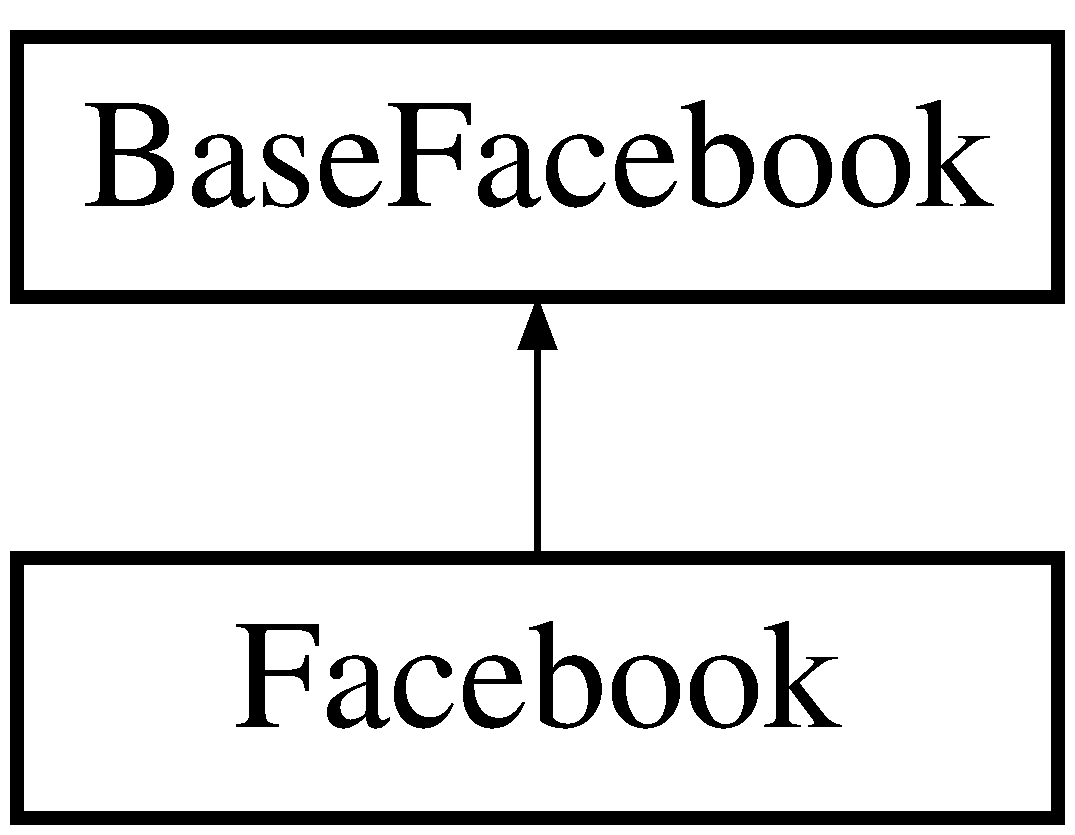
\includegraphics[height=2.000000cm]{class_facebook}
\end{center}
\end{figure}
\subsection*{Public Member Functions}
\begin{DoxyCompactItemize}
\item 
\hyperlink{class_facebook_a764229508830d143551d167e786c42f4}{\-\_\-\-\_\-construct} (\$config)
\end{DoxyCompactItemize}
\subsection*{Protected Member Functions}
\begin{DoxyCompactItemize}
\item 
\hyperlink{class_facebook_a8f094cc1c798c533283018a8100dffdf}{set\-Persistent\-Data} (\$key, \$value)
\end{DoxyCompactItemize}
\subsection*{Additional Inherited Members}


\subsection{Detailed Description}
Copyright 2011 \hyperlink{class_facebook}{Facebook}, Inc.

Licensed under the Apache License, Version 2.\-0 (the \char`\"{}\-License\char`\"{}); you may not use this file except in compliance with the License. You may obtain a copy of the License at \begin{DoxyVerb}http://www.apache.org/licenses/LICENSE-2.0
\end{DoxyVerb}


Unless required by applicable law or agreed to in writing, software distributed under the License is distributed on an \char`\"{}\-A\-S I\-S\char`\"{} B\-A\-S\-I\-S, W\-I\-T\-H\-O\-U\-T W\-A\-R\-R\-A\-N\-T\-I\-E\-S O\-R C\-O\-N\-D\-I\-T\-I\-O\-N\-S O\-F A\-N\-Y K\-I\-N\-D, either express or implied. See the License for the specific language governing permissions and limitations under the License. Extends the \hyperlink{class_base_facebook}{Base\-Facebook} class with the intent of using P\-H\-P sessions to store user ids and access tokens. 

\subsection{Constructor \& Destructor Documentation}
\hypertarget{class_facebook_a764229508830d143551d167e786c42f4}{\index{Facebook@{Facebook}!\-\_\-\-\_\-construct@{\-\_\-\-\_\-construct}}
\index{\-\_\-\-\_\-construct@{\-\_\-\-\_\-construct}!Facebook@{Facebook}}
\subsubsection[{\-\_\-\-\_\-construct}]{\setlength{\rightskip}{0pt plus 5cm}Facebook\-::\-\_\-\-\_\-construct (
\begin{DoxyParamCaption}
\item[{}]{\$config}
\end{DoxyParamCaption}
)}}\label{class_facebook_a764229508830d143551d167e786c42f4}
Identical to the parent constructor, except that we start a P\-H\-P session to store the user I\-D and access token if during the course of execution we discover them.


\begin{DoxyParams}[1]{Parameters}
Array & {\em \$config} & the application configuration. \\
\hline
\end{DoxyParams}
\begin{DoxySeeAlso}{See Also}
\hyperlink{class_base_facebook_af8ca4863484827e521f5052f5dfed642}{Base\-Facebook\-::\-\_\-\-\_\-construct} in facebook.\-php 
\end{DoxySeeAlso}


\subsection{Member Function Documentation}
\hypertarget{class_facebook_a8f094cc1c798c533283018a8100dffdf}{\index{Facebook@{Facebook}!set\-Persistent\-Data@{set\-Persistent\-Data}}
\index{set\-Persistent\-Data@{set\-Persistent\-Data}!Facebook@{Facebook}}
\subsubsection[{set\-Persistent\-Data}]{\setlength{\rightskip}{0pt plus 5cm}Facebook\-::set\-Persistent\-Data (
\begin{DoxyParamCaption}
\item[{}]{\$key, }
\item[{}]{\$value}
\end{DoxyParamCaption}
)\hspace{0.3cm}{\ttfamily [protected]}}}\label{class_facebook_a8f094cc1c798c533283018a8100dffdf}
Provides the implementations of the inherited abstract methods. The implementation uses P\-H\-P sessions to maintain a store for authorization codes, user ids, C\-S\-R\-F states, and access tokens. 

The documentation for this class was generated from the following file\-:\begin{DoxyCompactItemize}
\item 
facebook.\-php\end{DoxyCompactItemize}

\hypertarget{class_facebook_api_exception}{\section{Facebook\-Api\-Exception Class Reference}
\label{class_facebook_api_exception}\index{Facebook\-Api\-Exception@{Facebook\-Api\-Exception}}
}


Inherits Exception.

\subsection*{Public Member Functions}
\begin{DoxyCompactItemize}
\item 
\hyperlink{class_facebook_api_exception_a9e40d3c27096359975b952fe04752d19}{\-\_\-\-\_\-construct} (\$result)
\item 
\hyperlink{class_facebook_api_exception_ac6376ad18e5695a4ff443d4b6832f5f1}{get\-Result} ()
\item 
\hyperlink{class_facebook_api_exception_a6b119e3ab23ac69f3f51ee90aee6e688}{get\-Type} ()
\item 
\hyperlink{class_facebook_api_exception_a9c262b52fe807aad1c2770a0ad2ee919}{\-\_\-\-\_\-to\-String} ()
\end{DoxyCompactItemize}
\subsection*{Protected Attributes}
\begin{DoxyCompactItemize}
\item 
\hyperlink{class_facebook_api_exception_a7fb784ca5b949e79541f48d411cea829}{\$result}
\end{DoxyCompactItemize}


\subsection{Detailed Description}
Copyright 2011 \hyperlink{class_facebook}{Facebook}, Inc.

Licensed under the Apache License, Version 2.\-0 (the \char`\"{}\-License\char`\"{}); you may not use this file except in compliance with the License. You may obtain a copy of the License at \begin{DoxyVerb}http://www.apache.org/licenses/LICENSE-2.0
\end{DoxyVerb}


Unless required by applicable law or agreed to in writing, software distributed under the License is distributed on an \char`\"{}\-A\-S I\-S\char`\"{} B\-A\-S\-I\-S, W\-I\-T\-H\-O\-U\-T W\-A\-R\-R\-A\-N\-T\-I\-E\-S O\-R C\-O\-N\-D\-I\-T\-I\-O\-N\-S O\-F A\-N\-Y K\-I\-N\-D, either express or implied. See the License for the specific language governing permissions and limitations under the License. Thrown when an A\-P\-I call returns an exception.

\begin{DoxyAuthor}{Author}
Naitik Shah \href{mailto:naitik@facebook.com}{\tt naitik@facebook.\-com} 
\end{DoxyAuthor}


\subsection{Constructor \& Destructor Documentation}
\hypertarget{class_facebook_api_exception_a9e40d3c27096359975b952fe04752d19}{\index{Facebook\-Api\-Exception@{Facebook\-Api\-Exception}!\-\_\-\-\_\-construct@{\-\_\-\-\_\-construct}}
\index{\-\_\-\-\_\-construct@{\-\_\-\-\_\-construct}!FacebookApiException@{Facebook\-Api\-Exception}}
\subsubsection[{\-\_\-\-\_\-construct}]{\setlength{\rightskip}{0pt plus 5cm}Facebook\-Api\-Exception\-::\-\_\-\-\_\-construct (
\begin{DoxyParamCaption}
\item[{}]{\$result}
\end{DoxyParamCaption}
)}}\label{class_facebook_api_exception_a9e40d3c27096359975b952fe04752d19}
Make a new A\-P\-I Exception with the given result.


\begin{DoxyParams}[1]{Parameters}
array & {\em \$result} & The result from the A\-P\-I server \\
\hline
\end{DoxyParams}


\subsection{Member Function Documentation}
\hypertarget{class_facebook_api_exception_a9c262b52fe807aad1c2770a0ad2ee919}{\index{Facebook\-Api\-Exception@{Facebook\-Api\-Exception}!\-\_\-\-\_\-to\-String@{\-\_\-\-\_\-to\-String}}
\index{\-\_\-\-\_\-to\-String@{\-\_\-\-\_\-to\-String}!FacebookApiException@{Facebook\-Api\-Exception}}
\subsubsection[{\-\_\-\-\_\-to\-String}]{\setlength{\rightskip}{0pt plus 5cm}Facebook\-Api\-Exception\-::\-\_\-\-\_\-to\-String (
\begin{DoxyParamCaption}
{}
\end{DoxyParamCaption}
)}}\label{class_facebook_api_exception_a9c262b52fe807aad1c2770a0ad2ee919}
To make debugging easier.

\begin{DoxyReturn}{Returns}
string The string representation of the error 
\end{DoxyReturn}
\hypertarget{class_facebook_api_exception_ac6376ad18e5695a4ff443d4b6832f5f1}{\index{Facebook\-Api\-Exception@{Facebook\-Api\-Exception}!get\-Result@{get\-Result}}
\index{get\-Result@{get\-Result}!FacebookApiException@{Facebook\-Api\-Exception}}
\subsubsection[{get\-Result}]{\setlength{\rightskip}{0pt plus 5cm}Facebook\-Api\-Exception\-::get\-Result (
\begin{DoxyParamCaption}
{}
\end{DoxyParamCaption}
)}}\label{class_facebook_api_exception_ac6376ad18e5695a4ff443d4b6832f5f1}
Return the associated result object returned by the A\-P\-I server.

\begin{DoxyReturn}{Returns}
array The result from the A\-P\-I server 
\end{DoxyReturn}
\hypertarget{class_facebook_api_exception_a6b119e3ab23ac69f3f51ee90aee6e688}{\index{Facebook\-Api\-Exception@{Facebook\-Api\-Exception}!get\-Type@{get\-Type}}
\index{get\-Type@{get\-Type}!FacebookApiException@{Facebook\-Api\-Exception}}
\subsubsection[{get\-Type}]{\setlength{\rightskip}{0pt plus 5cm}Facebook\-Api\-Exception\-::get\-Type (
\begin{DoxyParamCaption}
{}
\end{DoxyParamCaption}
)}}\label{class_facebook_api_exception_a6b119e3ab23ac69f3f51ee90aee6e688}
Returns the associated type for the error. This will default to 'Exception' when a type is not available.

\begin{DoxyReturn}{Returns}
string 
\end{DoxyReturn}


\subsection{Member Data Documentation}
\hypertarget{class_facebook_api_exception_a7fb784ca5b949e79541f48d411cea829}{\index{Facebook\-Api\-Exception@{Facebook\-Api\-Exception}!\$result@{\$result}}
\index{\$result@{\$result}!FacebookApiException@{Facebook\-Api\-Exception}}
\subsubsection[{\$result}]{\setlength{\rightskip}{0pt plus 5cm}Facebook\-Api\-Exception\-::\$result\hspace{0.3cm}{\ttfamily [protected]}}}\label{class_facebook_api_exception_a7fb784ca5b949e79541f48d411cea829}
The result from the A\-P\-I server that represents the exception information. 

The documentation for this class was generated from the following file\-:\begin{DoxyCompactItemize}
\item 
base\-\_\-facebook.\-php\end{DoxyCompactItemize}

\hypertarget{classhtml2text}{\section{html2text Class Reference}
\label{classhtml2text}\index{html2text@{html2text}}
}
\subsection*{Public Member Functions}
\begin{DoxyCompactItemize}
\item 
\hyperlink{classhtml2text_ac404b5212f8b30c6b3b2e86806a5f5b2}{\-\_\-\-\_\-construct} (\$source=null)
\item 
\hyperlink{classhtml2text_abf3a1fc2ddd0622eaf181b68991cd382}{set\-\_\-html} (\$source, \$from\-\_\-file=false)
\item 
\hyperlink{classhtml2text_a160a9753434e61b3ff460860ca820c6d}{get\-Text} ()
\item 
\hyperlink{classhtml2text_aa1a63a82736ee37ea305e2e17b1b2cc9}{print\-\_\-text} ()
\item 
\hyperlink{classhtml2text_a65c9d6847400bced67eb0f82deb1784c}{p} ()
\item 
\hyperlink{classhtml2text_a426f32b8fc504be6eb0e2af96d9e11f6}{set\-\_\-allowed\-\_\-tags} (\$allowed\-\_\-tags= '')
\item 
\hyperlink{classhtml2text_afc4959f0839eccd625718914f879eabc}{set\-\_\-base\-\_\-url} (\$url= '')
\item 
\hyperlink{classhtml2text_adfcac63cc53ce5fd4f3ff2d72cf9a5c9}{\-\_\-convert} ()
\item 
\hyperlink{classhtml2text_a82ac6258106b2d8ad380dce11d9dddef}{\-\_\-build\-\_\-link\-\_\-list} (\$link, \$display)
\end{DoxyCompactItemize}
\subsection*{Public Attributes}
\begin{DoxyCompactItemize}
\item 
\hyperlink{classhtml2text_a891f6ae7d8de6312895706453fcda29f}{\$html}
\item 
\hyperlink{classhtml2text_a9f893148949046a51cefad452e88f4ab}{\$text}
\item 
\hyperlink{classhtml2text_a69cdbc42dd33f4215e4a655adaf24989}{\$width} = 70
\item 
\hyperlink{classhtml2text_aa5dbb9c672807ed8c4826b219aa2f22e}{\$search}
\item 
\hyperlink{classhtml2text_ab84fb8261392ce0f0d329dbffd0dc848}{\$replace}
\item 
\hyperlink{classhtml2text_a062ee8ef94be7191ef9dda3dba416891}{\$allowed\-\_\-tags} = ''
\item 
\hyperlink{classhtml2text_a2064bd23eca4e7eeb207ba23ca91613b}{\$url}
\item 
\hyperlink{classhtml2text_a98248146d367395beda0a99dce560690}{\$\-\_\-converted} = false
\item 
\hyperlink{classhtml2text_a2b0a222d507b5cb972acf2d10b4d9d3f}{\$\-\_\-link\-\_\-list} = ''
\item 
\hyperlink{classhtml2text_a12205ffda18f0cd0eb505b4d2332a32c}{\$\-\_\-link\-\_\-count} = 0
\end{DoxyCompactItemize}


\subsection{Detailed Description}
Takes H\-T\-M\-L and converts it to formatted, plain text.

Thanks to Alexander Krug (\href{http://www.krugar.de/}{\tt http\-://www.\-krugar.\-de/}) to pointing out and correcting an error in the regexp search array. Fixed 7/30/03.

Updated \hyperlink{classhtml2text_abf3a1fc2ddd0622eaf181b68991cd382}{set\-\_\-html()} function's file reading mechanism, 9/25/03.

Thanks to Joss Sanglier (\href{http://www.dancingbear.co.uk/}{\tt http\-://www.\-dancingbear.\-co.\-uk/}) for adding several more H\-T\-M\-L entity codes to the \$search and \$replace arrays. Updated 11/7/03.

Thanks to Darius Kasperavicius (\href{http://www.dar.dar.lt/}{\tt http\-://www.\-dar.\-dar.\-lt/}) for suggesting the addition of \$allowed\-\_\-tags and its supporting function (which I slightly modified). Updated 3/12/04.

Thanks to Justin Dearing for pointing out that a replacement for the 

tag was missing, and suggesting an appropriate fix. Updated 8/25/04.

Thanks to Mathieu Collas (\href{http://www.myefarm.com/}{\tt http\-://www.\-myefarm.\-com/}) for finding a display/formatting bug in the \hyperlink{classhtml2text_a82ac6258106b2d8ad380dce11d9dddef}{\-\_\-build\-\_\-link\-\_\-list()} function\-: email readers would show the left bracket and number (\char`\"{}\mbox{[}1\char`\"{}) as part of the rendered email address. Updated 12/16/04.

Thanks to Wojciech Bajon (\href{http://histeria.pl/}{\tt http\-://histeria.\-pl/}) for submitting code to handle relative links, which I hadn't considered. I modified his code a bit to handle normal H\-T\-T\-P links and M\-A\-I\-L\-T\-O links. Also for suggesting three additional H\-T\-M\-L entity codes to search for. Updated 03/02/05.

Thanks to Jacob Chandler for pointing out another link condition for the \hyperlink{classhtml2text_a82ac6258106b2d8ad380dce11d9dddef}{\-\_\-build\-\_\-link\-\_\-list()} function\-: \char`\"{}https\char`\"{}. Updated 04/06/05.

Thanks to Marc Bertrand (\href{http://www.dresdensky.com/}{\tt http\-://www.\-dresdensky.\-com/}) for suggesting a revision to the word wrapping functionality; if you specify a \$width of 0 or less, word wrapping will be ignored. Updated 11/02/06.

$\ast$$\ast$$\ast$ Big housecleaning updates below\-:

Thanks to Colin Brown (\href{http://www.sparkdriver.co.uk/}{\tt http\-://www.\-sparkdriver.\-co.\-uk/}) for suggesting the fix to handle  and blank lines (whitespace). Christian Basedau (\href{http://www.movetheweb.de/}{\tt http\-://www.\-movetheweb.\-de/}) also suggested the blank lines fix.

Special thanks to Marcus Bointon (\href{http://www.synchromedia.co.uk/}{\tt http\-://www.\-synchromedia.\-co.\-uk/}), Christian Basedau, Norbert Laposa (\href{http://ln5.co.uk/}{\tt http\-://ln5.\-co.\-uk/}), Bas van de Weijer, and Marijn van Butselaar for pointing out my glaring error in the 

handling. Marcus also supplied a host of fixes.

Thanks to Jeffrey Silverman (\href{http://www.newtnotes.com/}{\tt http\-://www.\-newtnotes.\-com/}) for pointing out that extra spaces should be compressed--a problem addressed with Marcus Bointon's fixes but that I had not yet incorporated.

Thanks to Daniel Schledermann (\href{http://www.typoconsult.dk/}{\tt http\-://www.\-typoconsult.\-dk/}) for suggesting a valuable fix with  tag handling.

Thanks to Wojciech Bajon (again!) for suggesting fixes and additions, including the  tag handling that Daniel Schledermann pointed out but that I had not yet incorporated. I haven't (yet) incorporated all of Wojciech's changes, though I may at some future time.

$\ast$$\ast$$\ast$ End of the housecleaning updates. Updated 08/08/07.

\begin{DoxyAuthor}{Author}
Jon Abernathy \href{mailto:jon@chuggnutt.com}{\tt jon@chuggnutt.\-com} 
\end{DoxyAuthor}
\begin{DoxyVersion}{Version}
1.\-0.\-0 
\end{DoxyVersion}
\begin{DoxySince}{Since}
P\-H\-P 4.\-0.\-2 
\end{DoxySince}


\subsection{Constructor \& Destructor Documentation}
\hypertarget{classhtml2text_ac404b5212f8b30c6b3b2e86806a5f5b2}{\index{html2text@{html2text}!\-\_\-\-\_\-construct@{\-\_\-\-\_\-construct}}
\index{\-\_\-\-\_\-construct@{\-\_\-\-\_\-construct}!html2text@{html2text}}
\subsubsection[{\-\_\-\-\_\-construct}]{\setlength{\rightskip}{0pt plus 5cm}html2text\-::\-\_\-\-\_\-construct (
\begin{DoxyParamCaption}
\item[{}]{\$source = {\ttfamily null}}
\end{DoxyParamCaption}
)}}\label{classhtml2text_ac404b5212f8b30c6b3b2e86806a5f5b2}
Constructor.

If the H\-T\-M\-L source string (or file) is supplied, the class will instantiate with that source propagated, all that has to be done it to call get\-\_\-text().


\begin{DoxyParams}[1]{Parameters}
string & {\em \$source} & H\-T\-M\-L content \\
\hline
boolean & {\em \$from\-\_\-file} & Indicates \$source is a file to pull content from  public \\
\hline
\end{DoxyParams}
\begin{DoxyReturn}{Returns}
void 
\end{DoxyReturn}


\subsection{Member Function Documentation}
\hypertarget{classhtml2text_a82ac6258106b2d8ad380dce11d9dddef}{\index{html2text@{html2text}!\-\_\-build\-\_\-link\-\_\-list@{\-\_\-build\-\_\-link\-\_\-list}}
\index{\-\_\-build\-\_\-link\-\_\-list@{\-\_\-build\-\_\-link\-\_\-list}!html2text@{html2text}}
\subsubsection[{\-\_\-build\-\_\-link\-\_\-list}]{\setlength{\rightskip}{0pt plus 5cm}html2text\-::\-\_\-build\-\_\-link\-\_\-list (
\begin{DoxyParamCaption}
\item[{}]{\$link, }
\item[{}]{\$display}
\end{DoxyParamCaption}
)}}\label{classhtml2text_a82ac6258106b2d8ad380dce11d9dddef}
Helper function called by preg\-\_\-replace() on link replacement.

Maintains an internal list of links to be displayed at the end of the text, with numeric indices to the original point in the text they appeared. Also makes an effort at identifying and handling absolute and relative links.


\begin{DoxyParams}[1]{Parameters}
string & {\em \$link} & U\-R\-L of the link \\
\hline
string & {\em \$display} & Part of the text to associate number with  private \\
\hline
\end{DoxyParams}
\begin{DoxyReturn}{Returns}
string 
\end{DoxyReturn}
\hypertarget{classhtml2text_adfcac63cc53ce5fd4f3ff2d72cf9a5c9}{\index{html2text@{html2text}!\-\_\-convert@{\-\_\-convert}}
\index{\-\_\-convert@{\-\_\-convert}!html2text@{html2text}}
\subsubsection[{\-\_\-convert}]{\setlength{\rightskip}{0pt plus 5cm}html2text\-::\-\_\-convert (
\begin{DoxyParamCaption}
{}
\end{DoxyParamCaption}
)}}\label{classhtml2text_adfcac63cc53ce5fd4f3ff2d72cf9a5c9}
Workhorse function that does actual conversion.

First performs custom tag replacement specified by \$search and \$replace arrays. Then strips any remaining H\-T\-M\-L tags, reduces whitespace and newlines to a readable format, and word wraps the text to \$width characters.

private \begin{DoxyReturn}{Returns}
void 
\end{DoxyReturn}
\hypertarget{classhtml2text_a160a9753434e61b3ff460860ca820c6d}{\index{html2text@{html2text}!get\-Text@{get\-Text}}
\index{get\-Text@{get\-Text}!html2text@{html2text}}
\subsubsection[{get\-Text}]{\setlength{\rightskip}{0pt plus 5cm}html2text\-::get\-Text (
\begin{DoxyParamCaption}
{}
\end{DoxyParamCaption}
)}}\label{classhtml2text_a160a9753434e61b3ff460860ca820c6d}
Returns the text, converted from H\-T\-M\-L.

public \begin{DoxyReturn}{Returns}
string 
\end{DoxyReturn}
\hypertarget{classhtml2text_a65c9d6847400bced67eb0f82deb1784c}{\index{html2text@{html2text}!p@{p}}
\index{p@{p}!html2text@{html2text}}
\subsubsection[{p}]{\setlength{\rightskip}{0pt plus 5cm}html2text\-::p (
\begin{DoxyParamCaption}
{}
\end{DoxyParamCaption}
)}}\label{classhtml2text_a65c9d6847400bced67eb0f82deb1784c}
Alias to \hyperlink{classhtml2text_aa1a63a82736ee37ea305e2e17b1b2cc9}{print\-\_\-text()}, operates identically.

public \begin{DoxyReturn}{Returns}
void 
\end{DoxyReturn}
\begin{DoxySeeAlso}{See Also}
\hyperlink{classhtml2text_aa1a63a82736ee37ea305e2e17b1b2cc9}{print\-\_\-text()} 
\end{DoxySeeAlso}
\hypertarget{classhtml2text_aa1a63a82736ee37ea305e2e17b1b2cc9}{\index{html2text@{html2text}!print\-\_\-text@{print\-\_\-text}}
\index{print\-\_\-text@{print\-\_\-text}!html2text@{html2text}}
\subsubsection[{print\-\_\-text}]{\setlength{\rightskip}{0pt plus 5cm}html2text\-::print\-\_\-text (
\begin{DoxyParamCaption}
{}
\end{DoxyParamCaption}
)}}\label{classhtml2text_aa1a63a82736ee37ea305e2e17b1b2cc9}
Prints the text, converted from H\-T\-M\-L.

public \begin{DoxyReturn}{Returns}
void 
\end{DoxyReturn}
\hypertarget{classhtml2text_a426f32b8fc504be6eb0e2af96d9e11f6}{\index{html2text@{html2text}!set\-\_\-allowed\-\_\-tags@{set\-\_\-allowed\-\_\-tags}}
\index{set\-\_\-allowed\-\_\-tags@{set\-\_\-allowed\-\_\-tags}!html2text@{html2text}}
\subsubsection[{set\-\_\-allowed\-\_\-tags}]{\setlength{\rightskip}{0pt plus 5cm}html2text\-::set\-\_\-allowed\-\_\-tags (
\begin{DoxyParamCaption}
\item[{}]{\$allowed\-\_\-tags = {\ttfamily ''}}
\end{DoxyParamCaption}
)}}\label{classhtml2text_a426f32b8fc504be6eb0e2af96d9e11f6}
Sets the allowed H\-T\-M\-L tags to pass through to the resulting text.

Tags should be in the form \char`\"{}$<$p$>$\char`\"{}, with no corresponding closing tag.

public \begin{DoxyReturn}{Returns}
void 
\end{DoxyReturn}
\hypertarget{classhtml2text_afc4959f0839eccd625718914f879eabc}{\index{html2text@{html2text}!set\-\_\-base\-\_\-url@{set\-\_\-base\-\_\-url}}
\index{set\-\_\-base\-\_\-url@{set\-\_\-base\-\_\-url}!html2text@{html2text}}
\subsubsection[{set\-\_\-base\-\_\-url}]{\setlength{\rightskip}{0pt plus 5cm}html2text\-::set\-\_\-base\-\_\-url (
\begin{DoxyParamCaption}
\item[{}]{\$url = {\ttfamily ''}}
\end{DoxyParamCaption}
)}}\label{classhtml2text_afc4959f0839eccd625718914f879eabc}
Sets a base U\-R\-L to handle relative links.

public \begin{DoxyReturn}{Returns}
void 
\end{DoxyReturn}
\hypertarget{classhtml2text_abf3a1fc2ddd0622eaf181b68991cd382}{\index{html2text@{html2text}!set\-\_\-html@{set\-\_\-html}}
\index{set\-\_\-html@{set\-\_\-html}!html2text@{html2text}}
\subsubsection[{set\-\_\-html}]{\setlength{\rightskip}{0pt plus 5cm}html2text\-::set\-\_\-html (
\begin{DoxyParamCaption}
\item[{}]{\$source, }
\item[{}]{\$from\-\_\-file = {\ttfamily false}}
\end{DoxyParamCaption}
)}}\label{classhtml2text_abf3a1fc2ddd0622eaf181b68991cd382}
Loads source H\-T\-M\-L into memory, either from \$source string or a file.


\begin{DoxyParams}[1]{Parameters}
string & {\em \$source} & H\-T\-M\-L content \\
\hline
boolean & {\em \$from\-\_\-file} & Indicates \$source is a file to pull content from  public \\
\hline
\end{DoxyParams}
\begin{DoxyReturn}{Returns}
void 
\end{DoxyReturn}


\subsection{Member Data Documentation}
\hypertarget{classhtml2text_a98248146d367395beda0a99dce560690}{\index{html2text@{html2text}!\$\-\_\-converted@{\$\-\_\-converted}}
\index{\$\-\_\-converted@{\$\-\_\-converted}!html2text@{html2text}}
\subsubsection[{\$\-\_\-converted}]{\setlength{\rightskip}{0pt plus 5cm}boolean html2text\-::\$\-\_\-converted = false}}\label{classhtml2text_a98248146d367395beda0a99dce560690}
Indicates whether content in the \$html variable has been converted yet.

private \begin{DoxySeeAlso}{See Also}
\hyperlink{classhtml2text_a891f6ae7d8de6312895706453fcda29f}{\$html}, \hyperlink{classhtml2text_a9f893148949046a51cefad452e88f4ab}{\$text} 
\end{DoxySeeAlso}
\hypertarget{classhtml2text_a12205ffda18f0cd0eb505b4d2332a32c}{\index{html2text@{html2text}!\$\-\_\-link\-\_\-count@{\$\-\_\-link\-\_\-count}}
\index{\$\-\_\-link\-\_\-count@{\$\-\_\-link\-\_\-count}!html2text@{html2text}}
\subsubsection[{\$\-\_\-link\-\_\-count}]{\setlength{\rightskip}{0pt plus 5cm}integer html2text\-::\$\-\_\-link\-\_\-count = 0}}\label{classhtml2text_a12205ffda18f0cd0eb505b4d2332a32c}
Number of valid links detected in the text, used for plain text display (rendered similar to footnotes).

private \begin{DoxySeeAlso}{See Also}
\hyperlink{classhtml2text_a82ac6258106b2d8ad380dce11d9dddef}{\-\_\-build\-\_\-link\-\_\-list()} 
\end{DoxySeeAlso}
\hypertarget{classhtml2text_a2b0a222d507b5cb972acf2d10b4d9d3f}{\index{html2text@{html2text}!\$\-\_\-link\-\_\-list@{\$\-\_\-link\-\_\-list}}
\index{\$\-\_\-link\-\_\-list@{\$\-\_\-link\-\_\-list}!html2text@{html2text}}
\subsubsection[{\$\-\_\-link\-\_\-list}]{\setlength{\rightskip}{0pt plus 5cm}string html2text\-::\$\-\_\-link\-\_\-list = ''}}\label{classhtml2text_a2b0a222d507b5cb972acf2d10b4d9d3f}
Contains U\-R\-L addresses from links to be rendered in plain text.

private \begin{DoxySeeAlso}{See Also}
\hyperlink{classhtml2text_a82ac6258106b2d8ad380dce11d9dddef}{\-\_\-build\-\_\-link\-\_\-list()} 
\end{DoxySeeAlso}
\hypertarget{classhtml2text_a062ee8ef94be7191ef9dda3dba416891}{\index{html2text@{html2text}!\$allowed\-\_\-tags@{\$allowed\-\_\-tags}}
\index{\$allowed\-\_\-tags@{\$allowed\-\_\-tags}!html2text@{html2text}}
\subsubsection[{\$allowed\-\_\-tags}]{\setlength{\rightskip}{0pt plus 5cm}string html2text\-::\$allowed\-\_\-tags = ''}}\label{classhtml2text_a062ee8ef94be7191ef9dda3dba416891}
Contains a list of H\-T\-M\-L tags to allow in the resulting text.

public \begin{DoxySeeAlso}{See Also}
\hyperlink{classhtml2text_a426f32b8fc504be6eb0e2af96d9e11f6}{set\-\_\-allowed\-\_\-tags()} 
\end{DoxySeeAlso}
\hypertarget{classhtml2text_a891f6ae7d8de6312895706453fcda29f}{\index{html2text@{html2text}!\$html@{\$html}}
\index{\$html@{\$html}!html2text@{html2text}}
\subsubsection[{\$html}]{\setlength{\rightskip}{0pt plus 5cm}string html2text\-::\$html}}\label{classhtml2text_a891f6ae7d8de6312895706453fcda29f}
Contains the H\-T\-M\-L content to convert.

public \hypertarget{classhtml2text_ab84fb8261392ce0f0d329dbffd0dc848}{\index{html2text@{html2text}!\$replace@{\$replace}}
\index{\$replace@{\$replace}!html2text@{html2text}}
\subsubsection[{\$replace}]{\setlength{\rightskip}{0pt plus 5cm}array html2text\-::\$replace}}\label{classhtml2text_ab84fb8261392ce0f0d329dbffd0dc848}
List of pattern replacements corresponding to patterns searched.

public \begin{DoxySeeAlso}{See Also}
\hyperlink{classhtml2text_aa5dbb9c672807ed8c4826b219aa2f22e}{\$search} 
\end{DoxySeeAlso}
\hypertarget{classhtml2text_aa5dbb9c672807ed8c4826b219aa2f22e}{\index{html2text@{html2text}!\$search@{\$search}}
\index{\$search@{\$search}!html2text@{html2text}}
\subsubsection[{\$search}]{\setlength{\rightskip}{0pt plus 5cm}array html2text\-::\$search}}\label{classhtml2text_aa5dbb9c672807ed8c4826b219aa2f22e}
List of preg$\ast$ regular expression patterns to search for, used in conjunction with \$replace.

public \begin{DoxySeeAlso}{See Also}
\hyperlink{classhtml2text_ab84fb8261392ce0f0d329dbffd0dc848}{\$replace} 
\end{DoxySeeAlso}
\hypertarget{classhtml2text_a9f893148949046a51cefad452e88f4ab}{\index{html2text@{html2text}!\$text@{\$text}}
\index{\$text@{\$text}!html2text@{html2text}}
\subsubsection[{\$text}]{\setlength{\rightskip}{0pt plus 5cm}string html2text\-::\$text}}\label{classhtml2text_a9f893148949046a51cefad452e88f4ab}
Contains the converted, formatted text.

public \hypertarget{classhtml2text_a2064bd23eca4e7eeb207ba23ca91613b}{\index{html2text@{html2text}!\$url@{\$url}}
\index{\$url@{\$url}!html2text@{html2text}}
\subsubsection[{\$url}]{\setlength{\rightskip}{0pt plus 5cm}string html2text\-::\$url}}\label{classhtml2text_a2064bd23eca4e7eeb207ba23ca91613b}
Contains the base U\-R\-L that relative links should resolve to.

public \hypertarget{classhtml2text_a69cdbc42dd33f4215e4a655adaf24989}{\index{html2text@{html2text}!\$width@{\$width}}
\index{\$width@{\$width}!html2text@{html2text}}
\subsubsection[{\$width}]{\setlength{\rightskip}{0pt plus 5cm}integer html2text\-::\$width = 70}}\label{classhtml2text_a69cdbc42dd33f4215e4a655adaf24989}
Maximum width of the formatted text, in columns.

Set this value to 0 (or less) to ignore word wrapping and not constrain text to a fixed-\/width column.

public 

The documentation for this class was generated from the following file\-:\begin{DoxyCompactItemize}
\item 
class.\-html2text.\-php\end{DoxyCompactItemize}

\hypertarget{class_i_p_c_o}{\section{I\-P\-C\-O Class Reference}
\label{class_i_p_c_o}\index{I\-P\-C\-O@{I\-P\-C\-O}}
}
\subsection*{Public Member Functions}
\begin{DoxyCompactItemize}
\item 
\hyperlink{class_i_p_c_o_ae0e86b06b253b50ff01d37f9c190f046}{get\-Template\-Class\-Name} (\$s\-Identifier)
\end{DoxyCompactItemize}


\subsection{Detailed Description}
Inline php compilator.

This library takes a template file, parses it, and returns valid and optimised php code. Choosing to recompile a file, saving the result, or re-\/using a previous version is not included. Thus you need to make your own wrapper to handle the caching of the \hyperlink{class_i_p_c_o}{I\-P\-C\-O} output.

\begin{DoxyAuthor}{Author}
Jelle Voet 
\end{DoxyAuthor}
\begin{DoxyVersion}{Version}
0.\-1.\-0 Beta 
\end{DoxyVersion}


\subsection{Member Function Documentation}
\hypertarget{class_i_p_c_o_ae0e86b06b253b50ff01d37f9c190f046}{\index{I\-P\-C\-O@{I\-P\-C\-O}!get\-Template\-Class\-Name@{get\-Template\-Class\-Name}}
\index{get\-Template\-Class\-Name@{get\-Template\-Class\-Name}!IPCO@{I\-P\-C\-O}}
\subsubsection[{get\-Template\-Class\-Name}]{\setlength{\rightskip}{0pt plus 5cm}I\-P\-C\-O\-::get\-Template\-Class\-Name (
\begin{DoxyParamCaption}
\item[{}]{\$s\-Identifier}
\end{DoxyParamCaption}
)}}\label{class_i_p_c_o_ae0e86b06b253b50ff01d37f9c190f046}
Generate a valid classname for the given identifier.


\begin{DoxyParams}[1]{Parameters}
string & {\em \$s\-Identifier} & \\
\hline
\end{DoxyParams}
\begin{DoxyReturn}{Returns}
string 
\end{DoxyReturn}


The documentation for this class was generated from the following file\-:\begin{DoxyCompactItemize}
\item 
ipco.\-php\end{DoxyCompactItemize}

\hypertarget{class_o_auth_signature_method}{\section{O\-Auth\-Signature\-Method Class Reference}
\label{class_o_auth_signature_method}\index{O\-Auth\-Signature\-Method@{O\-Auth\-Signature\-Method}}
}
Inheritance diagram for O\-Auth\-Signature\-Method\-:\begin{figure}[H]
\begin{center}
\leavevmode
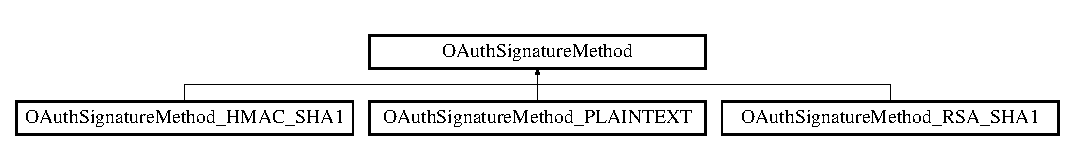
\includegraphics[height=1.575246cm]{class_o_auth_signature_method}
\end{center}
\end{figure}
\subsection*{Public Member Functions}
\begin{DoxyCompactItemize}
\item 
\hyperlink{class_o_auth_signature_method_ad42c31991e3a144fd7ac46bb268df758}{get\-Name} ()
\item 
\hyperlink{class_o_auth_signature_method_a72f2a7ccf70732c7359c2539815bf32d}{build\-Signature} (O\-Auth\-Request \$o\-Request, O\-Auth\-Consumer \$o\-Consumer, O\-Auth\-Token \$o\-Token=null)
\item 
\hyperlink{class_o_auth_signature_method_aedd9a3e183880b2d1ea47fe06c988240}{check\-Signature} (O\-Auth\-Request \$o\-Request, O\-Auth\-Consumer \$o\-Consumer, O\-Auth\-Token \$o\-Token=null, \$s\-Signature)
\end{DoxyCompactItemize}


\subsection{Detailed Description}
A class for implementing a Signature Method See section 9 (\char`\"{}\-Signing Requests\char`\"{}) in the spec 

\subsection{Member Function Documentation}
\hypertarget{class_o_auth_signature_method_a72f2a7ccf70732c7359c2539815bf32d}{\index{O\-Auth\-Signature\-Method@{O\-Auth\-Signature\-Method}!build\-Signature@{build\-Signature}}
\index{build\-Signature@{build\-Signature}!OAuthSignatureMethod@{O\-Auth\-Signature\-Method}}
\subsubsection[{build\-Signature}]{\setlength{\rightskip}{0pt plus 5cm}O\-Auth\-Signature\-Method\-::build\-Signature (
\begin{DoxyParamCaption}
\item[{O\-Auth\-Request}]{\$o\-Request, }
\item[{O\-Auth\-Consumer}]{\$o\-Consumer, }
\item[{O\-Auth\-Token}]{\$o\-Token = {\ttfamily null}}
\end{DoxyParamCaption}
)\hspace{0.3cm}{\ttfamily [abstract]}}}\label{class_o_auth_signature_method_a72f2a7ccf70732c7359c2539815bf32d}
Build up the signature N\-O\-T\-E\-: The output of this function M\-U\-S\-T N\-O\-T be urlencoded. the encoding is handled in O\-Auth\-Request when the final request is serialized


\begin{DoxyParams}[1]{Parameters}
O\-Auth\-Request & {\em \$request} & \\
\hline
O\-Auth\-Consumer & {\em \$consumer} & \\
\hline
O\-Auth\-Token & {\em \$token} & \\
\hline
\end{DoxyParams}
\begin{DoxyReturn}{Returns}
string 
\end{DoxyReturn}
\hypertarget{class_o_auth_signature_method_aedd9a3e183880b2d1ea47fe06c988240}{\index{O\-Auth\-Signature\-Method@{O\-Auth\-Signature\-Method}!check\-Signature@{check\-Signature}}
\index{check\-Signature@{check\-Signature}!OAuthSignatureMethod@{O\-Auth\-Signature\-Method}}
\subsubsection[{check\-Signature}]{\setlength{\rightskip}{0pt plus 5cm}O\-Auth\-Signature\-Method\-::check\-Signature (
\begin{DoxyParamCaption}
\item[{O\-Auth\-Request}]{\$o\-Request, }
\item[{O\-Auth\-Consumer}]{\$o\-Consumer, }
\item[{O\-Auth\-Token}]{\$o\-Token = {\ttfamily null}, }
\item[{}]{\$s\-Signature}
\end{DoxyParamCaption}
)}}\label{class_o_auth_signature_method_aedd9a3e183880b2d1ea47fe06c988240}
Verifies that a given signature is correct


\begin{DoxyParams}[1]{Parameters}
O\-Auth\-Request & {\em \$request} & \\
\hline
O\-Auth\-Consumer & {\em \$consumer} & \\
\hline
O\-Auth\-Token & {\em \$token} & \\
\hline
string & {\em \$signature} & \\
\hline
\end{DoxyParams}
\begin{DoxyReturn}{Returns}
bool 
\end{DoxyReturn}
\hypertarget{class_o_auth_signature_method_ad42c31991e3a144fd7ac46bb268df758}{\index{O\-Auth\-Signature\-Method@{O\-Auth\-Signature\-Method}!get\-Name@{get\-Name}}
\index{get\-Name@{get\-Name}!OAuthSignatureMethod@{O\-Auth\-Signature\-Method}}
\subsubsection[{get\-Name}]{\setlength{\rightskip}{0pt plus 5cm}O\-Auth\-Signature\-Method\-::get\-Name (
\begin{DoxyParamCaption}
{}
\end{DoxyParamCaption}
)\hspace{0.3cm}{\ttfamily [abstract]}}}\label{class_o_auth_signature_method_ad42c31991e3a144fd7ac46bb268df758}
Needs to return the name of the Signature Method (ie H\-M\-A\-C-\/\-S\-H\-A1)

\begin{DoxyReturn}{Returns}
string 
\end{DoxyReturn}


The documentation for this class was generated from the following file\-:\begin{DoxyCompactItemize}
\item 
oauth\-\_\-signatureproviders.\-php\end{DoxyCompactItemize}

\hypertarget{class_o_auth_signature_method___h_m_a_c___s_h_a1}{\section{O\-Auth\-Signature\-Method\-\_\-\-H\-M\-A\-C\-\_\-\-S\-H\-A1 Class Reference}
\label{class_o_auth_signature_method___h_m_a_c___s_h_a1}\index{O\-Auth\-Signature\-Method\-\_\-\-H\-M\-A\-C\-\_\-\-S\-H\-A1@{O\-Auth\-Signature\-Method\-\_\-\-H\-M\-A\-C\-\_\-\-S\-H\-A1}}
}
Inheritance diagram for O\-Auth\-Signature\-Method\-\_\-\-H\-M\-A\-C\-\_\-\-S\-H\-A1\-:\begin{figure}[H]
\begin{center}
\leavevmode
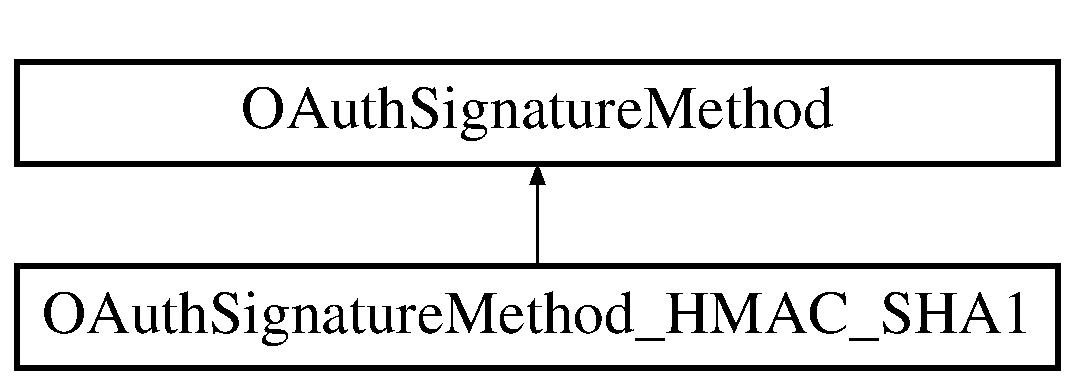
\includegraphics[height=2.000000cm]{class_o_auth_signature_method___h_m_a_c___s_h_a1}
\end{center}
\end{figure}
\subsection*{Additional Inherited Members}


\subsection{Detailed Description}
The H\-M\-A\-C-\/\-S\-H\-A1 signature method uses the H\-M\-A\-C-\/\-S\-H\-A1 signature algorithm as defined in \mbox{[}R\-F\-C2104\mbox{]} where the Signature Base String is the text and the key is the concatenated values (each first encoded per Parameter \hyperlink{class_encoding}{Encoding}) of the Consumer Secret and Token Secret, separated by an '\&' character (A\-S\-C\-I\-I code 38) even if empty.
\begin{DoxyItemize}
\item Chapter 9.\-2 (\char`\"{}\-H\-M\-A\-C-\/\-S\-H\-A1\char`\"{}) 
\end{DoxyItemize}

The documentation for this class was generated from the following file\-:\begin{DoxyCompactItemize}
\item 
oauth\-\_\-signatureproviders.\-php\end{DoxyCompactItemize}

\hypertarget{class_o_auth_signature_method___p_l_a_i_n_t_e_x_t}{\section{O\-Auth\-Signature\-Method\-\_\-\-P\-L\-A\-I\-N\-T\-E\-X\-T Class Reference}
\label{class_o_auth_signature_method___p_l_a_i_n_t_e_x_t}\index{O\-Auth\-Signature\-Method\-\_\-\-P\-L\-A\-I\-N\-T\-E\-X\-T@{O\-Auth\-Signature\-Method\-\_\-\-P\-L\-A\-I\-N\-T\-E\-X\-T}}
}
Inheritance diagram for O\-Auth\-Signature\-Method\-\_\-\-P\-L\-A\-I\-N\-T\-E\-X\-T\-:\begin{figure}[H]
\begin{center}
\leavevmode
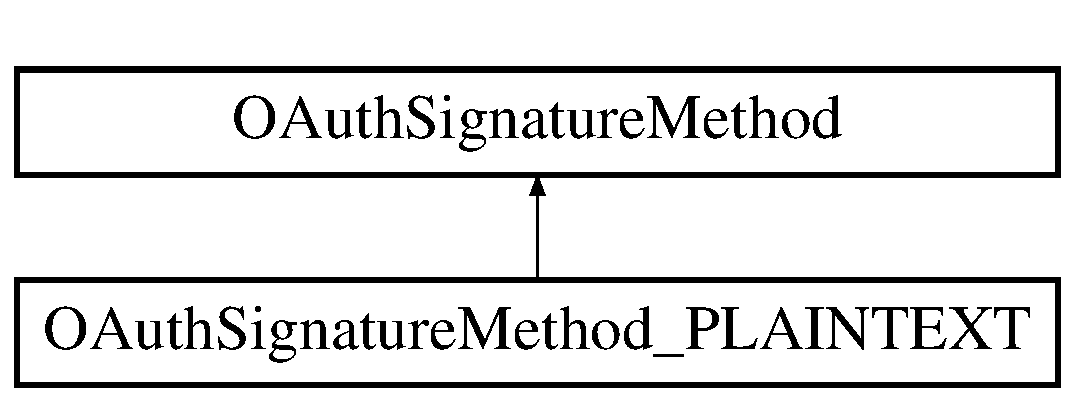
\includegraphics[height=2.000000cm]{class_o_auth_signature_method___p_l_a_i_n_t_e_x_t}
\end{center}
\end{figure}
\subsection*{Public Member Functions}
\begin{DoxyCompactItemize}
\item 
\hyperlink{class_o_auth_signature_method___p_l_a_i_n_t_e_x_t_ab1140b04de8f27425d3bedfde97ac2a0}{build\-Signature} (O\-Auth\-Request \$o\-Request, O\-Auth\-Consumer \$o\-Consumer, O\-Auth\-Token \$o\-Token=null)
\end{DoxyCompactItemize}


\subsection{Detailed Description}
The P\-L\-A\-I\-N\-T\-E\-X\-T method does not provide any security protection and S\-H\-O\-U\-L\-D only be used over a secure channel such as H\-T\-T\-P\-S. It does not use the Signature Base String.
\begin{DoxyItemize}
\item Chapter 9.\-4 (\char`\"{}\-P\-L\-A\-I\-N\-T\-E\-X\-T\char`\"{}) 
\end{DoxyItemize}

\subsection{Member Function Documentation}
\hypertarget{class_o_auth_signature_method___p_l_a_i_n_t_e_x_t_ab1140b04de8f27425d3bedfde97ac2a0}{\index{O\-Auth\-Signature\-Method\-\_\-\-P\-L\-A\-I\-N\-T\-E\-X\-T@{O\-Auth\-Signature\-Method\-\_\-\-P\-L\-A\-I\-N\-T\-E\-X\-T}!build\-Signature@{build\-Signature}}
\index{build\-Signature@{build\-Signature}!OAuthSignatureMethod_PLAINTEXT@{O\-Auth\-Signature\-Method\-\_\-\-P\-L\-A\-I\-N\-T\-E\-X\-T}}
\subsubsection[{build\-Signature}]{\setlength{\rightskip}{0pt plus 5cm}O\-Auth\-Signature\-Method\-\_\-\-P\-L\-A\-I\-N\-T\-E\-X\-T\-::build\-Signature (
\begin{DoxyParamCaption}
\item[{O\-Auth\-Request}]{\$o\-Request, }
\item[{O\-Auth\-Consumer}]{\$o\-Consumer, }
\item[{O\-Auth\-Token}]{\$o\-Token = {\ttfamily null}}
\end{DoxyParamCaption}
)}}\label{class_o_auth_signature_method___p_l_a_i_n_t_e_x_t_ab1140b04de8f27425d3bedfde97ac2a0}
oauth\-\_\-signature is set to the concatenated encoded values of the Consumer Secret and Token Secret, separated by a '\&' character (A\-S\-C\-I\-I code 38), even if either secret is empty. The result M\-U\-S\-T be encoded again.
\begin{DoxyItemize}
\item Chapter 9.\-4.\-1 (\char`\"{}\-Generating Signatures\char`\"{})
\end{DoxyItemize}

Please note that the second encoding M\-U\-S\-T N\-O\-T happen in the Signature\-Method, as O\-Auth\-Request handles this! 

The documentation for this class was generated from the following file\-:\begin{DoxyCompactItemize}
\item 
oauth\-\_\-signatureproviders.\-php\end{DoxyCompactItemize}

\hypertarget{class_o_auth_signature_method___r_s_a___s_h_a1}{\section{O\-Auth\-Signature\-Method\-\_\-\-R\-S\-A\-\_\-\-S\-H\-A1 Class Reference}
\label{class_o_auth_signature_method___r_s_a___s_h_a1}\index{O\-Auth\-Signature\-Method\-\_\-\-R\-S\-A\-\_\-\-S\-H\-A1@{O\-Auth\-Signature\-Method\-\_\-\-R\-S\-A\-\_\-\-S\-H\-A1}}
}
Inheritance diagram for O\-Auth\-Signature\-Method\-\_\-\-R\-S\-A\-\_\-\-S\-H\-A1\-:\begin{figure}[H]
\begin{center}
\leavevmode
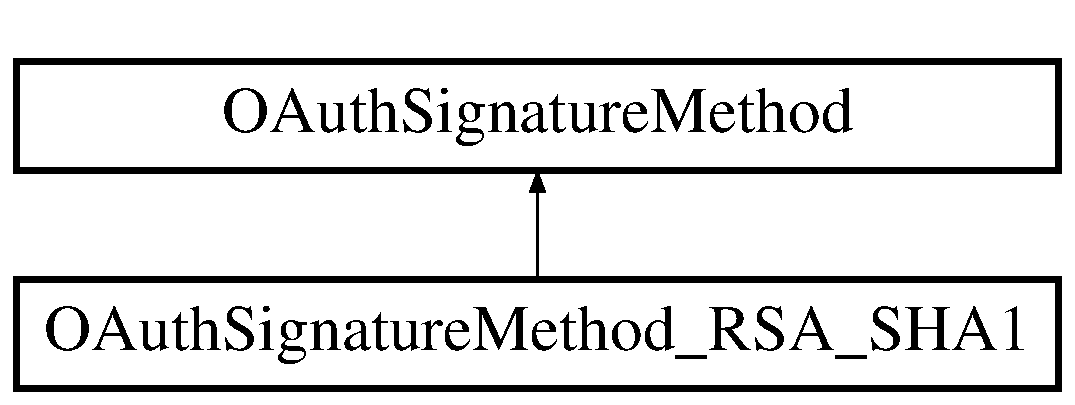
\includegraphics[height=2.000000cm]{class_o_auth_signature_method___r_s_a___s_h_a1}
\end{center}
\end{figure}
\subsection*{Additional Inherited Members}


\subsection{Detailed Description}
The R\-S\-A-\/\-S\-H\-A1 signature method uses the R\-S\-A\-S\-S\-A-\/\-P\-K\-C\-S1-\/v1\-\_\-5 signature algorithm as defined in \mbox{[}R\-F\-C3447\mbox{]} section 8.\-2 (more simply known as P\-K\-C\-S\#1), using S\-H\-A-\/1 as the hash function for E\-M\-S\-A-\/\-P\-K\-C\-S1-\/v1\-\_\-5. It is assumed that the Consumer has provided its R\-S\-A public key in a verified way to the Service Provider, in a manner which is beyond the scope of this specification.
\begin{DoxyItemize}
\item Chapter 9.\-3 (\char`\"{}\-R\-S\-A-\/\-S\-H\-A1\char`\"{}) 
\end{DoxyItemize}

The documentation for this class was generated from the following file\-:\begin{DoxyCompactItemize}
\item 
oauth\-\_\-signatureproviders.\-php\end{DoxyCompactItemize}

\hypertarget{class_request}{\section{Request Class Reference}
\label{class_request}\index{Request@{Request}}
}
\subsection*{Static Public Member Functions}
\begin{DoxyCompactItemize}
\item 
static \hyperlink{class_request_a0552dcea819c77f239bb6db060e17b47}{init} ()
\item 
static \hyperlink{class_request_a8d58147bb9572424021c44b0ebb3f85a}{is\-Http} ()
\item 
static \hyperlink{class_request_afab6f7cb93efa72b28f3e8b2eba901dd}{is\-Https} ()
\item 
static \hyperlink{class_request_a23d8c8dfb64e8f03ba857e83887a3f93}{scheme} ()
\item 
static \hyperlink{class_request_a512dd9b95abef2346ad3af2e593d10c1}{user} ()
\item 
static \hyperlink{class_request_a1ad0dec68fffe32c3b59e5130b63c1ba}{password} ()
\item 
static \hyperlink{class_request_a291eeae48e2675a5301279b0e1b8d8e2}{host} (\$b\-Server=false)
\item 
static \hyperlink{class_request_a495e06b9d24638c678259b6f3aefbcd6}{port} ()
\item 
static \hyperlink{class_request_aca04f9b433bb568c10d32ee114a0d02c}{base} ()
\item 
static \hyperlink{class_request_a64f9327ac4a815b3f114d50fd6ba521b}{offset} ()
\item 
static \hyperlink{class_request_a6b69986e47c94186cce2336f11ad1f6e}{root} ()
\item 
static \hyperlink{class_request_ae1725b521b1833602f3f554566142c51}{path} ()
\item 
static \hyperlink{class_request_ada5f08ac6d1754ad0cc7312c10b8c9a3}{mapping} (\$n\-Index=-\/1)
\item 
static \hyperlink{class_request_abf1e0caab3f4027d508eec81489b260b}{url} ()
\item 
static \hyperlink{class_request_a4d6813e2943a1ced4ae7159e3a382695}{method} ()
\item 
static \hyperlink{class_request_a12099938e1500f4559b32b833de2088e}{useragent} ()
\item 
static \hyperlink{class_request_abe8f53d7d11ac4eaa65928a1f8adee77}{compressions} ()
\item 
static \hyperlink{class_request_a8cbc39d7e3f77bd7ed2000e59f2859f7}{compression\-Support} (\$s\-Compression)
\item 
static \hyperlink{class_request_aced74b3005542537ca7f3b4592545cbb}{last\-Modified} ()
\item 
static \hyperlink{class_request_ac55d4834ecde0026dfacef5d9545a29c}{e\-Tag} ()
\item 
static \hyperlink{class_request_af0cfa5de39cd1b78dd183f8755c5881a}{get} (\$m\-Index, \$m\-Default=null)
\item 
static \hyperlink{class_request_ab2b509ddd1e625547bd79a8f207670e3}{post} (\$m\-Index, \$m\-Default=null)
\item 
static \hyperlink{class_request_af0d98675f85be7ee4fca80e18942693b}{session} (\$m\-Index, \$m\-Default=null)
\item 
static \hyperlink{class_request_ad6b7fe8e73dd7eed912086488002ddd0}{cookie} (\$m\-Index, \$m\-Default=null)
\item 
static \hyperlink{class_request_a2817486e88b192ef552ebca4c62d70af}{detail} ()
\item 
static \hyperlink{class_request_a865d084fee04c82e9704b1144e5b4c84}{make} (\$s\-Path, array \$a\-Get=array())
\end{DoxyCompactItemize}


\subsection{Detailed Description}
This class hold the request data for the current request. Before using it, you should make sure to call \hyperlink{class_request_a0552dcea819c77f239bb6db060e17b47}{Request\-::init()}. If this class is used as part of Watena, this will be done for you.

\begin{DoxyAuthor}{Author}
Jelle Voet 
\end{DoxyAuthor}
\begin{DoxyVersion}{Version}
0.\-1.\-0 
\end{DoxyVersion}


\subsection{Member Function Documentation}
\hypertarget{class_request_aca04f9b433bb568c10d32ee114a0d02c}{\index{Request@{Request}!base@{base}}
\index{base@{base}!Request@{Request}}
\subsubsection[{base}]{\setlength{\rightskip}{0pt plus 5cm}static Request\-::base (
\begin{DoxyParamCaption}
{}
\end{DoxyParamCaption}
)\hspace{0.3cm}{\ttfamily [static]}, {\ttfamily [final]}}}\label{class_request_aca04f9b433bb568c10d32ee114a0d02c}
Retrieve the base portion of the current request.

\begin{DoxySeeAlso}{See Also}
Request\-::protocol() 

\hyperlink{class_request_a512dd9b95abef2346ad3af2e593d10c1}{Request\-::user()} 

\hyperlink{class_request_a1ad0dec68fffe32c3b59e5130b63c1ba}{Request\-::password()} 

\hyperlink{class_request_a291eeae48e2675a5301279b0e1b8d8e2}{Request\-::host()} 

\hyperlink{class_request_a495e06b9d24638c678259b6f3aefbcd6}{Request\-::port()} 
\end{DoxySeeAlso}
\begin{DoxyReturn}{Returns}
string http\mbox{[}s\mbox{]}\-://\mbox{[}user\mbox{[}\-:password\mbox{]}@\mbox{]}example.\-com\mbox{[}\-:80\mbox{]} 
\end{DoxyReturn}
\hypertarget{class_request_abe8f53d7d11ac4eaa65928a1f8adee77}{\index{Request@{Request}!compressions@{compressions}}
\index{compressions@{compressions}!Request@{Request}}
\subsubsection[{compressions}]{\setlength{\rightskip}{0pt plus 5cm}static Request\-::compressions (
\begin{DoxyParamCaption}
{}
\end{DoxyParamCaption}
)\hspace{0.3cm}{\ttfamily [static]}, {\ttfamily [final]}}}\label{class_request_abe8f53d7d11ac4eaa65928a1f8adee77}
Retrieve an array with lowercase allowed compression techniques of teh request. The content of the array is parsed from the Accept-\/\-Encoding header, and split by comma.

\begin{DoxyReturn}{Returns}
array 
\end{DoxyReturn}
\hypertarget{class_request_a8cbc39d7e3f77bd7ed2000e59f2859f7}{\index{Request@{Request}!compression\-Support@{compression\-Support}}
\index{compression\-Support@{compression\-Support}!Request@{Request}}
\subsubsection[{compression\-Support}]{\setlength{\rightskip}{0pt plus 5cm}static Request\-::compression\-Support (
\begin{DoxyParamCaption}
\item[{}]{\$s\-Compression}
\end{DoxyParamCaption}
)\hspace{0.3cm}{\ttfamily [static]}, {\ttfamily [final]}}}\label{class_request_a8cbc39d7e3f77bd7ed2000e59f2859f7}
Check if the given compression is supported for the current request.

\begin{DoxySeeAlso}{See Also}
Request\-::compression() 
\end{DoxySeeAlso}

\begin{DoxyParams}[1]{Parameters}
string & {\em \$s\-Compression} & \\
\hline
\end{DoxyParams}
\begin{DoxyReturn}{Returns}
boolean 
\end{DoxyReturn}
\hypertarget{class_request_ad6b7fe8e73dd7eed912086488002ddd0}{\index{Request@{Request}!cookie@{cookie}}
\index{cookie@{cookie}!Request@{Request}}
\subsubsection[{cookie}]{\setlength{\rightskip}{0pt plus 5cm}static Request\-::cookie (
\begin{DoxyParamCaption}
\item[{}]{\$m\-Index, }
\item[{}]{\$m\-Default = {\ttfamily null}}
\end{DoxyParamCaption}
)\hspace{0.3cm}{\ttfamily [static]}, {\ttfamily [final]}}}\label{class_request_ad6b7fe8e73dd7eed912086488002ddd0}
Retrieve the specified value from the current \$\-\_\-\-C\-O\-O\-K\-I\-E. You can specify as you would when using array\-\_\-value(). If the specified index does not exist, \$m\-Default will be returned

\begin{DoxySeeAlso}{See Also}
array\-\_\-value() 
\end{DoxySeeAlso}

\begin{DoxyParams}[1]{Parameters}
mixed & {\em \$m\-Index} & The index of the required value. \\
\hline
mixed & {\em \$m\-Default} & Default value when index does not exist. \\
\hline
\end{DoxyParams}
\begin{DoxyReturn}{Returns}
mixed The value specified by \$m\-Index in \$\-\_\-\-C\-O\-O\-K\-I\-E, of \$m\-Default. 
\end{DoxyReturn}
\hypertarget{class_request_a2817486e88b192ef552ebca4c62d70af}{\index{Request@{Request}!detail@{detail}}
\index{detail@{detail}!Request@{Request}}
\subsubsection[{detail}]{\setlength{\rightskip}{0pt plus 5cm}static Request\-::detail (
\begin{DoxyParamCaption}
{}
\end{DoxyParamCaption}
)\hspace{0.3cm}{\ttfamily [static]}, {\ttfamily [final]}}}\label{class_request_a2817486e88b192ef552ebca4c62d70af}
Retrieve the full detailed string containing the current request state. Currently only the \$\-\_\-\-G\-E\-T parameters are appended. (not \$\-\_\-\-P\-O\-S\-T, \$\-\_\-\-C\-O\-O\-K\-I\-E, \$\-\_\-\-S\-E\-S\-S\-I\-O\-N) This is the concatenation of \hyperlink{class_request_a4d6813e2943a1ced4ae7159e3a382695}{Request\-::method()}, \hyperlink{class_request_abf1e0caab3f4027d508eec81489b260b}{Request\-::url()}, \hyperlink{class_request_af0cfa5de39cd1b78dd183f8755c5881a}{Request\-::get()}, \hyperlink{class_request_a12099938e1500f4559b32b833de2088e}{Request\-::useragent()}.

\begin{DoxySeeAlso}{See Also}
\hyperlink{class_request_a4d6813e2943a1ced4ae7159e3a382695}{Request\-::method()} 

\hyperlink{class_request_abf1e0caab3f4027d508eec81489b260b}{Request\-::url()} 

\hyperlink{class_request_af0cfa5de39cd1b78dd183f8755c5881a}{Request\-::get()} 

\hyperlink{class_request_a12099938e1500f4559b32b833de2088e}{Request\-::useragent()} 
\end{DoxySeeAlso}
\begin{DoxyReturn}{Returns}
string \mbox{[}G\-E\-T\mbox{]} http\mbox{[}s\mbox{]}\-://\mbox{[}user\mbox{[}\-:password\mbox{]}@\mbox{]}example.\-com\mbox{[}\-:80\mbox{]}\mbox{[}/path-\/to-\/install\mbox{]}/\mbox{[}path/mapping\mbox{]}?\mbox{[}param0=foo\&param1=bar\mbox{]} (useragent) 
\end{DoxyReturn}
\hypertarget{class_request_ac55d4834ecde0026dfacef5d9545a29c}{\index{Request@{Request}!e\-Tag@{e\-Tag}}
\index{e\-Tag@{e\-Tag}!Request@{Request}}
\subsubsection[{e\-Tag}]{\setlength{\rightskip}{0pt plus 5cm}static Request\-::e\-Tag (
\begin{DoxyParamCaption}
{}
\end{DoxyParamCaption}
)\hspace{0.3cm}{\ttfamily [static]}, {\ttfamily [final]}}}\label{class_request_ac55d4834ecde0026dfacef5d9545a29c}
Retrieve the if\-\_\-none\-\_\-match information from the current request. This header is only valid when sent on a repeated request where the earlier response had the etag header. You can check this value later on to validate the requirement to sent possibly cached content.

\begin{DoxyReturn}{Returns}
string$|$null 
\end{DoxyReturn}
\hypertarget{class_request_af0cfa5de39cd1b78dd183f8755c5881a}{\index{Request@{Request}!get@{get}}
\index{get@{get}!Request@{Request}}
\subsubsection[{get}]{\setlength{\rightskip}{0pt plus 5cm}static Request\-::get (
\begin{DoxyParamCaption}
\item[{}]{\$m\-Index, }
\item[{}]{\$m\-Default = {\ttfamily null}}
\end{DoxyParamCaption}
)\hspace{0.3cm}{\ttfamily [static]}, {\ttfamily [final]}}}\label{class_request_af0cfa5de39cd1b78dd183f8755c5881a}
Retrieve the specified value from the current \$\-\_\-\-G\-E\-T. You can specify as you would when using array\-\_\-value(). If the specified index does not exist, \$m\-Default will be returned

\begin{DoxySeeAlso}{See Also}
array\-\_\-value() 
\end{DoxySeeAlso}

\begin{DoxyParams}[1]{Parameters}
mixed & {\em \$m\-Index} & The index of the required value. \\
\hline
mixed & {\em \$m\-Default} & Default value when index does not exist. \\
\hline
\end{DoxyParams}
\begin{DoxyReturn}{Returns}
mixed The value specified by \$m\-Index in \$\-\_\-\-G\-E\-T, of \$m\-Default. 
\end{DoxyReturn}
\hypertarget{class_request_a291eeae48e2675a5301279b0e1b8d8e2}{\index{Request@{Request}!host@{host}}
\index{host@{host}!Request@{Request}}
\subsubsection[{host}]{\setlength{\rightskip}{0pt plus 5cm}static Request\-::host (
\begin{DoxyParamCaption}
\item[{}]{\$b\-Server = {\ttfamily false}}
\end{DoxyParamCaption}
)\hspace{0.3cm}{\ttfamily [static]}, {\ttfamily [final]}}}\label{class_request_a291eeae48e2675a5301279b0e1b8d8e2}
Retrieve the lowercase hostname of the current request. Optionally you can try to retrieve the actual server-\/name as specified on the server config. If not required, the value returned will be the host-\/portion of the request. The return value is based on \$\-\_\-\-S\-E\-R\-V\-E\-R\mbox{[}'S\-E\-R\-V\-E\-R\-\_\-\-N\-A\-M\-E'\mbox{]} or \$\-\_\-\-S\-E\-R\-V\-E\-R\mbox{[}'H\-T\-T\-P\-\_\-\-P\-O\-S\-T'\mbox{]}.


\begin{DoxyParams}[1]{Parameters}
boolean & {\em \$b\-Server} & Set to true if you want the internal server-\/name. \\
\hline
\end{DoxyParams}
\begin{DoxyReturn}{Returns}
string Returns lowercase \$\-\_\-\-S\-E\-R\-V\-E\-R\mbox{[}'H\-T\-T\-P\-\_\-\-H\-O\-S\-T'\mbox{]} or \$\-\_\-\-S\-E\-R\-V\-E\-R\mbox{[}'S\-E\-R\-V\-E\-R\-\_\-\-N\-A\-M\-E'\mbox{]}. (default\-: localhost) 
\end{DoxyReturn}
\hypertarget{class_request_a0552dcea819c77f239bb6db060e17b47}{\index{Request@{Request}!init@{init}}
\index{init@{init}!Request@{Request}}
\subsubsection[{init}]{\setlength{\rightskip}{0pt plus 5cm}static Request\-::init (
\begin{DoxyParamCaption}
{}
\end{DoxyParamCaption}
)\hspace{0.3cm}{\ttfamily [static]}, {\ttfamily [final]}}}\label{class_request_a0552dcea819c77f239bb6db060e17b47}
Initialize and cache the correct values for the current request. \hypertarget{class_request_a8d58147bb9572424021c44b0ebb3f85a}{\index{Request@{Request}!is\-Http@{is\-Http}}
\index{is\-Http@{is\-Http}!Request@{Request}}
\subsubsection[{is\-Http}]{\setlength{\rightskip}{0pt plus 5cm}static Request\-::is\-Http (
\begin{DoxyParamCaption}
{}
\end{DoxyParamCaption}
)\hspace{0.3cm}{\ttfamily [static]}, {\ttfamily [final]}}}\label{class_request_a8d58147bb9572424021c44b0ebb3f85a}
Determine if the current request is not using a secured protocol. This method is the opposite of \hyperlink{class_request_afab6f7cb93efa72b28f3e8b2eba901dd}{Request\-::is\-Https()}. The return value is based on \$\-\_\-\-S\-E\-R\-V\-E\-R\mbox{[}'H\-T\-T\-P\-S'\mbox{]} and will influence the behaviour of Request\-::protocol() and \hyperlink{class_request_a495e06b9d24638c678259b6f3aefbcd6}{Request\-::port()}.

\begin{DoxySeeAlso}{See Also}
\hyperlink{class_request_afab6f7cb93efa72b28f3e8b2eba901dd}{Request\-::is\-Https()} 

\hyperlink{class_request_a23d8c8dfb64e8f03ba857e83887a3f93}{Request\-::scheme()} 

\hyperlink{class_request_a495e06b9d24638c678259b6f3aefbcd6}{Request\-::port()} 
\end{DoxySeeAlso}
\begin{DoxyReturn}{Returns}
boolean Indicates if the current request is not using https. (default\-: true) 
\end{DoxyReturn}
\hypertarget{class_request_afab6f7cb93efa72b28f3e8b2eba901dd}{\index{Request@{Request}!is\-Https@{is\-Https}}
\index{is\-Https@{is\-Https}!Request@{Request}}
\subsubsection[{is\-Https}]{\setlength{\rightskip}{0pt plus 5cm}static Request\-::is\-Https (
\begin{DoxyParamCaption}
{}
\end{DoxyParamCaption}
)\hspace{0.3cm}{\ttfamily [static]}, {\ttfamily [final]}}}\label{class_request_afab6f7cb93efa72b28f3e8b2eba901dd}
Determine if the current request is using a secured protocol. This method is the opposite of \hyperlink{class_request_a8d58147bb9572424021c44b0ebb3f85a}{Request\-::is\-Http()}. The return value is based on \$\-\_\-\-S\-E\-R\-V\-E\-R\mbox{[}'H\-T\-T\-P\-S'\mbox{]} and will influence the behaviour of Request\-::protocol() and \hyperlink{class_request_a495e06b9d24638c678259b6f3aefbcd6}{Request\-::port()}.

\begin{DoxySeeAlso}{See Also}
\hyperlink{class_request_afab6f7cb93efa72b28f3e8b2eba901dd}{Request\-::is\-Https()} 

\hyperlink{class_request_a23d8c8dfb64e8f03ba857e83887a3f93}{Request\-::scheme()} 

\hyperlink{class_request_a495e06b9d24638c678259b6f3aefbcd6}{Request\-::port()} 
\end{DoxySeeAlso}
\begin{DoxyReturn}{Returns}
boolean Indicates of the current request is using https. (default\-: false) 
\end{DoxyReturn}
\hypertarget{class_request_aced74b3005542537ca7f3b4592545cbb}{\index{Request@{Request}!last\-Modified@{last\-Modified}}
\index{last\-Modified@{last\-Modified}!Request@{Request}}
\subsubsection[{last\-Modified}]{\setlength{\rightskip}{0pt plus 5cm}static Request\-::last\-Modified (
\begin{DoxyParamCaption}
{}
\end{DoxyParamCaption}
)\hspace{0.3cm}{\ttfamily [static]}, {\ttfamily [final]}}}\label{class_request_aced74b3005542537ca7f3b4592545cbb}
Retrieve the if\-\_\-modified\-\_\-since information from the current request. This header is only valid when sent on a repeated request where the earlier response had the last-\/modified header. You can check this value later on to validate the requirement to sent possibly cached content.

\begin{DoxyReturn}{Returns}
string$|$null 
\end{DoxyReturn}
\hypertarget{class_request_a865d084fee04c82e9704b1144e5b4c84}{\index{Request@{Request}!make@{make}}
\index{make@{make}!Request@{Request}}
\subsubsection[{make}]{\setlength{\rightskip}{0pt plus 5cm}static Request\-::make (
\begin{DoxyParamCaption}
\item[{}]{\$s\-Path, }
\item[{array}]{\$a\-Get = {\ttfamily array()}}
\end{DoxyParamCaption}
)\hspace{0.3cm}{\ttfamily [static]}, {\ttfamily [final]}}}\label{class_request_a865d084fee04c82e9704b1144e5b4c84}
Make a local url instance using the same 'root' portion as the current request.

\begin{DoxySeeAlso}{See Also}
\hyperlink{class_request_a6b69986e47c94186cce2336f11ad1f6e}{Request\-::root()} 
\end{DoxySeeAlso}

\begin{DoxyParams}[1]{Parameters}
string & {\em \$s\-Path} & \\
\hline
array & {\em \$a\-Get} & \\
\hline
\end{DoxyParams}
\begin{DoxyReturn}{Returns}
Url 
\end{DoxyReturn}
\hypertarget{class_request_ada5f08ac6d1754ad0cc7312c10b8c9a3}{\index{Request@{Request}!mapping@{mapping}}
\index{mapping@{mapping}!Request@{Request}}
\subsubsection[{mapping}]{\setlength{\rightskip}{0pt plus 5cm}static Request\-::mapping (
\begin{DoxyParamCaption}
\item[{}]{\$n\-Index = {\ttfamily -\/1}}
\end{DoxyParamCaption}
)\hspace{0.3cm}{\ttfamily [static]}, {\ttfamily [final]}}}\label{class_request_ada5f08ac6d1754ad0cc7312c10b8c9a3}
Retrieve the mapping of the current request. The mapping here is defined as the path split on forward slashes without the empty values. If an index is specified the mapping at given index is returned, or 'null' if not set.


\begin{DoxyParams}[1]{Parameters}
int & {\em \$n\-Index} & The index of the mapping part you require. \\
\hline
\end{DoxyParams}
\begin{DoxyReturn}{Returns}
array$|$string$|$null An array with the mapping $|$ The mapping you specified with \$n\-Index $|$ nothing if nothing found 
\end{DoxyReturn}
\hypertarget{class_request_a4d6813e2943a1ced4ae7159e3a382695}{\index{Request@{Request}!method@{method}}
\index{method@{method}!Request@{Request}}
\subsubsection[{method}]{\setlength{\rightskip}{0pt plus 5cm}static Request\-::method (
\begin{DoxyParamCaption}
{}
\end{DoxyParamCaption}
)\hspace{0.3cm}{\ttfamily [static]}, {\ttfamily [final]}}}\label{class_request_a4d6813e2943a1ced4ae7159e3a382695}
Retrieve the uppercase request-\/method of the current request. If no request-\/method is specified, this will default to G\-E\-T. The return values is based on \$\-\_\-\-S\-E\-R\-V\-E\-R\mbox{[}'R\-E\-Q\-U\-E\-S\-T\-\_\-\-M\-E\-T\-H\-O\-D'\mbox{]}.

\begin{DoxyReturn}{Returns}
string De method used for the data of the current request. (default\-: 'G\-E\-T') 
\end{DoxyReturn}
\hypertarget{class_request_a64f9327ac4a815b3f114d50fd6ba521b}{\index{Request@{Request}!offset@{offset}}
\index{offset@{offset}!Request@{Request}}
\subsubsection[{offset}]{\setlength{\rightskip}{0pt plus 5cm}static Request\-::offset (
\begin{DoxyParamCaption}
{}
\end{DoxyParamCaption}
)\hspace{0.3cm}{\ttfamily [static]}, {\ttfamily [final]}}}\label{class_request_a64f9327ac4a815b3f114d50fd6ba521b}
Retrieve the offset portion of the current request. The offset is defined as the difference between the base and the root url for the current request and is not fixed 'per install'.

\begin{DoxyReturn}{Returns}
string The path to the webroot for this install. /path-\/to-\/install 
\end{DoxyReturn}
\hypertarget{class_request_a1ad0dec68fffe32c3b59e5130b63c1ba}{\index{Request@{Request}!password@{password}}
\index{password@{password}!Request@{Request}}
\subsubsection[{password}]{\setlength{\rightskip}{0pt plus 5cm}static Request\-::password (
\begin{DoxyParamCaption}
{}
\end{DoxyParamCaption}
)\hspace{0.3cm}{\ttfamily [static]}, {\ttfamily [final]}}}\label{class_request_a1ad0dec68fffe32c3b59e5130b63c1ba}
Retrievethe http-\/authentication password of the current request. The return value is based on \$\-\_\-\-S\-E\-R\-V\-E\-R\mbox{[}'P\-H\-P\-\_\-\-A\-U\-T\-H\-\_\-\-P\-A\-S\-S'\mbox{]}.

\begin{DoxyReturn}{Returns}
string The password portion of the current request. (default\-: '') 
\end{DoxyReturn}
\hypertarget{class_request_ae1725b521b1833602f3f554566142c51}{\index{Request@{Request}!path@{path}}
\index{path@{path}!Request@{Request}}
\subsubsection[{path}]{\setlength{\rightskip}{0pt plus 5cm}static Request\-::path (
\begin{DoxyParamCaption}
{}
\end{DoxyParamCaption}
)\hspace{0.3cm}{\ttfamily [static]}, {\ttfamily [final]}}}\label{class_request_ae1725b521b1833602f3f554566142c51}
Retrieve the path portion of the current request. The path is defined as the as the posfix after the offset and thus contains the actual mapping with the install starting from the root. When no mapping is found, this will always return '/'.

\begin{DoxyReturn}{Returns}
string The mapping for the current request. /path/mapping (default\-: '/') 
\end{DoxyReturn}
\hypertarget{class_request_a495e06b9d24638c678259b6f3aefbcd6}{\index{Request@{Request}!port@{port}}
\index{port@{port}!Request@{Request}}
\subsubsection[{port}]{\setlength{\rightskip}{0pt plus 5cm}static Request\-::port (
\begin{DoxyParamCaption}
{}
\end{DoxyParamCaption}
)\hspace{0.3cm}{\ttfamily [static]}, {\ttfamily [final]}}}\label{class_request_a495e06b9d24638c678259b6f3aefbcd6}
Retrieve the portnumber of the current request. The return value is based on \$\-\_\-\-S\-E\-R\-V\-E\-R\mbox{[}S\-E\-R\-V\-E\-R\-\_\-\-P\-O\-R\-T\mbox{]}. If no port is specified, this will default to 80 for http and 443 for https.

\begin{DoxySeeAlso}{See Also}
\hyperlink{class_request_a8d58147bb9572424021c44b0ebb3f85a}{Request\-::is\-Http()} 

\hyperlink{class_request_afab6f7cb93efa72b28f3e8b2eba901dd}{Request\-::is\-Https()} 
\end{DoxySeeAlso}
\begin{DoxyReturn}{Returns}
int The port number of the current request. (default based on protocol\-: 80 or 443) 
\end{DoxyReturn}
\hypertarget{class_request_ab2b509ddd1e625547bd79a8f207670e3}{\index{Request@{Request}!post@{post}}
\index{post@{post}!Request@{Request}}
\subsubsection[{post}]{\setlength{\rightskip}{0pt plus 5cm}static Request\-::post (
\begin{DoxyParamCaption}
\item[{}]{\$m\-Index, }
\item[{}]{\$m\-Default = {\ttfamily null}}
\end{DoxyParamCaption}
)\hspace{0.3cm}{\ttfamily [static]}, {\ttfamily [final]}}}\label{class_request_ab2b509ddd1e625547bd79a8f207670e3}
Retrieve the specified value from the current \$\-\_\-\-P\-O\-S\-T. You can specify as you would when using array\-\_\-value(). If the specified index does not exist, \$m\-Default will be returned

\begin{DoxySeeAlso}{See Also}
array\-\_\-value() 
\end{DoxySeeAlso}

\begin{DoxyParams}[1]{Parameters}
mixed & {\em \$m\-Index} & The index of the required value. \\
\hline
mixed & {\em \$m\-Default} & Default value when index does not exist. \\
\hline
\end{DoxyParams}
\begin{DoxyReturn}{Returns}
mixed The value specified by \$m\-Index in \$\-\_\-\-P\-O\-S\-T, of \$m\-Default. 
\end{DoxyReturn}
\hypertarget{class_request_a6b69986e47c94186cce2336f11ad1f6e}{\index{Request@{Request}!root@{root}}
\index{root@{root}!Request@{Request}}
\subsubsection[{root}]{\setlength{\rightskip}{0pt plus 5cm}static Request\-::root (
\begin{DoxyParamCaption}
{}
\end{DoxyParamCaption}
)\hspace{0.3cm}{\ttfamily [static]}, {\ttfamily [final]}}}\label{class_request_a6b69986e47c94186cce2336f11ad1f6e}
Retrieve the root portion of the current request. This is the concatenation of \hyperlink{class_request_aca04f9b433bb568c10d32ee114a0d02c}{Request\-::base()} and \hyperlink{class_request_a64f9327ac4a815b3f114d50fd6ba521b}{Request\-::offset()}.

\begin{DoxySeeAlso}{See Also}
\hyperlink{class_request_aca04f9b433bb568c10d32ee114a0d02c}{Request\-::base()} 

\hyperlink{class_request_a64f9327ac4a815b3f114d50fd6ba521b}{Request\-::offset()} 
\end{DoxySeeAlso}
\begin{DoxyReturn}{Returns}
string http\mbox{[}s\mbox{]}\-://\mbox{[}user\mbox{[}\-:password\mbox{]}@\mbox{]}example.\-com\mbox{[}\-:80\mbox{]}\mbox{[}/path-\/to-\/install\mbox{]} 
\end{DoxyReturn}
\hypertarget{class_request_a23d8c8dfb64e8f03ba857e83887a3f93}{\index{Request@{Request}!scheme@{scheme}}
\index{scheme@{scheme}!Request@{Request}}
\subsubsection[{scheme}]{\setlength{\rightskip}{0pt plus 5cm}static Request\-::scheme (
\begin{DoxyParamCaption}
{}
\end{DoxyParamCaption}
)\hspace{0.3cm}{\ttfamily [static]}, {\ttfamily [final]}}}\label{class_request_a23d8c8dfb64e8f03ba857e83887a3f93}
Retrieve the scheme/protocol of the current request. Currently the only two protocols supported are 'http' and 'https'. The return value is based on \hyperlink{class_request_a8d58147bb9572424021c44b0ebb3f85a}{Request\-::is\-Http()} and \hyperlink{class_request_afab6f7cb93efa72b28f3e8b2eba901dd}{Request\-::is\-Https()}.

\begin{DoxySeeAlso}{See Also}
\hyperlink{class_request_a8d58147bb9572424021c44b0ebb3f85a}{Request\-::is\-Http()} 

\hyperlink{class_request_afab6f7cb93efa72b28f3e8b2eba901dd}{Request\-::is\-Https()} 
\end{DoxySeeAlso}
\begin{DoxyReturn}{Returns}
string Return value should be 'http' or 'https'. (default\-: 'http') 
\end{DoxyReturn}
\hypertarget{class_request_af0d98675f85be7ee4fca80e18942693b}{\index{Request@{Request}!session@{session}}
\index{session@{session}!Request@{Request}}
\subsubsection[{session}]{\setlength{\rightskip}{0pt plus 5cm}static Request\-::session (
\begin{DoxyParamCaption}
\item[{}]{\$m\-Index, }
\item[{}]{\$m\-Default = {\ttfamily null}}
\end{DoxyParamCaption}
)\hspace{0.3cm}{\ttfamily [static]}, {\ttfamily [final]}}}\label{class_request_af0d98675f85be7ee4fca80e18942693b}
Retrieve the specified value from the current \$\-\_\-\-S\-E\-S\-S\-I\-O\-N. You can specify as you would when using array\-\_\-value(). If the specified index does not exist, \$m\-Default will be returned

\begin{DoxySeeAlso}{See Also}
array\-\_\-value() 
\end{DoxySeeAlso}

\begin{DoxyParams}[1]{Parameters}
mixed & {\em \$m\-Index} & The index of the required value. \\
\hline
mixed & {\em \$m\-Default} & Default value when index does not exist. \\
\hline
\end{DoxyParams}
\begin{DoxyReturn}{Returns}
mixed The value specified by \$m\-Index in \$\-\_\-\-S\-E\-S\-S\-I\-O\-N, of \$m\-Default. 
\end{DoxyReturn}
\hypertarget{class_request_abf1e0caab3f4027d508eec81489b260b}{\index{Request@{Request}!url@{url}}
\index{url@{url}!Request@{Request}}
\subsubsection[{url}]{\setlength{\rightskip}{0pt plus 5cm}static Request\-::url (
\begin{DoxyParamCaption}
{}
\end{DoxyParamCaption}
)\hspace{0.3cm}{\ttfamily [static]}, {\ttfamily [final]}}}\label{class_request_abf1e0caab3f4027d508eec81489b260b}
Retrieve the full url of the current request. This is the concatenation of \hyperlink{class_request_a6b69986e47c94186cce2336f11ad1f6e}{Request\-::root()} and \hyperlink{class_request_ae1725b521b1833602f3f554566142c51}{Request\-::path()}.

\begin{DoxySeeAlso}{See Also}
\hyperlink{class_request_a6b69986e47c94186cce2336f11ad1f6e}{Request\-::root()} 

\hyperlink{class_request_ae1725b521b1833602f3f554566142c51}{Request\-::path()} 
\end{DoxySeeAlso}
\begin{DoxyReturn}{Returns}
string http\mbox{[}s\mbox{]}\-://\mbox{[}user\mbox{[}\-:password\mbox{]}@\mbox{]}example.\-com\mbox{[}\-:80\mbox{]}\mbox{[}/path-\/to-\/install\mbox{]}/\mbox{[}path/mapping\mbox{]} 
\end{DoxyReturn}
\hypertarget{class_request_a512dd9b95abef2346ad3af2e593d10c1}{\index{Request@{Request}!user@{user}}
\index{user@{user}!Request@{Request}}
\subsubsection[{user}]{\setlength{\rightskip}{0pt plus 5cm}static Request\-::user (
\begin{DoxyParamCaption}
{}
\end{DoxyParamCaption}
)\hspace{0.3cm}{\ttfamily [static]}, {\ttfamily [final]}}}\label{class_request_a512dd9b95abef2346ad3af2e593d10c1}
Retrieve the http-\/authentication user of the current request. The return value is based on \$\-\_\-\-S\-E\-R\-V\-E\-R\mbox{[}'P\-H\-P\-\_\-\-A\-U\-T\-H\-\_\-\-U\-S\-E\-R'\mbox{]}.

\begin{DoxyReturn}{Returns}
string The user portion of the current request. (default\-: '') 
\end{DoxyReturn}
\hypertarget{class_request_a12099938e1500f4559b32b833de2088e}{\index{Request@{Request}!useragent@{useragent}}
\index{useragent@{useragent}!Request@{Request}}
\subsubsection[{useragent}]{\setlength{\rightskip}{0pt plus 5cm}static Request\-::useragent (
\begin{DoxyParamCaption}
{}
\end{DoxyParamCaption}
)\hspace{0.3cm}{\ttfamily [static]}, {\ttfamily [final]}}}\label{class_request_a12099938e1500f4559b32b833de2088e}
Retrieve the useragent of the current request. This will automatically save the useragent to a session. If a subsequent request with useragent $\ast$ / $\ast$ should occur, the session-\/value will be used instead. If no useragent is specified, this will default to 'Unknown'.

\begin{DoxyReturn}{Returns}
string The persistent useragent data from the previous and current requests. 
\end{DoxyReturn}


The documentation for this class was generated from the following file\-:\begin{DoxyCompactItemize}
\item 
static.\-request.\-php\end{DoxyCompactItemize}

\hypertarget{class_session_guard}{\section{Session\-Guard Class Reference}
\label{class_session_guard}\index{Session\-Guard@{Session\-Guard}}
}


\subsection{Detailed Description}
This class protects our session

\begin{DoxyAuthor}{Author}
Jelle Voet 
\end{DoxyAuthor}
\begin{DoxyVersion}{Version}
1.\-0.\-0 R\-C1 
\end{DoxyVersion}


The documentation for this class was generated from the following files\-:\begin{DoxyCompactItemize}
\item 
class.\-sessionguard.\-php\item 
static.\-sessionguard.\-php\end{DoxyCompactItemize}

\hypertarget{class_t_m_x___ajax_page}{\section{T\-M\-X\-\_\-\-Ajax\-Page Class Reference}
\label{class_t_m_x___ajax_page}\index{T\-M\-X\-\_\-\-Ajax\-Page@{T\-M\-X\-\_\-\-Ajax\-Page}}
}


Inherits T\-M\-D\-\_\-\-Page.

\subsection*{Public Member Functions}
\begin{DoxyCompactItemize}
\item 
\hyperlink{class_t_m_x___ajax_page_a387f7ddcd307f49c5fe17700052a937b}{\-\_\-\-\_\-construct} (T\-M\-X\-\_\-\-Response \$o\-Response)
\end{DoxyCompactItemize}
\subsection*{Protected Member Functions}
\begin{DoxyCompactItemize}
\item 
\hyperlink{class_t_m_x___ajax_page_a9c28ea558dd714e20a5e7174cd6f7411}{Set\-Headers} ()
\item 
\hyperlink{class_t_m_x___ajax_page_ac98232f9db9c62594da2ababa6920edb}{Get\-Content} ()
\end{DoxyCompactItemize}


\subsection{Detailed Description}
Class that outputs the T\-M\-X-\/response

\begin{DoxyAuthor}{Author}
Voet Jelle -\/ Tom\-O-\/design 
\end{DoxyAuthor}
\begin{DoxyVersion}{Version}
1.\-0.\-0 beta 
\end{DoxyVersion}


\subsection{Constructor \& Destructor Documentation}
\hypertarget{class_t_m_x___ajax_page_a387f7ddcd307f49c5fe17700052a937b}{\index{T\-M\-X\-\_\-\-Ajax\-Page@{T\-M\-X\-\_\-\-Ajax\-Page}!\-\_\-\-\_\-construct@{\-\_\-\-\_\-construct}}
\index{\-\_\-\-\_\-construct@{\-\_\-\-\_\-construct}!TMX_AjaxPage@{T\-M\-X\-\_\-\-Ajax\-Page}}
\subsubsection[{\-\_\-\-\_\-construct}]{\setlength{\rightskip}{0pt plus 5cm}T\-M\-X\-\_\-\-Ajax\-Page\-::\-\_\-\-\_\-construct (
\begin{DoxyParamCaption}
\item[{T\-M\-X\-\_\-\-Response}]{\$o\-Response}
\end{DoxyParamCaption}
)}}\label{class_t_m_x___ajax_page_a387f7ddcd307f49c5fe17700052a937b}
Create a new Ajax\-Page to output your T\-M\-X request


\begin{DoxyParams}[1]{Parameters}
T\-M\-X\-\_\-\-Response & {\em \$o\-Response} & \\
\hline
\end{DoxyParams}


\subsection{Member Function Documentation}
\hypertarget{class_t_m_x___ajax_page_ac98232f9db9c62594da2ababa6920edb}{\index{T\-M\-X\-\_\-\-Ajax\-Page@{T\-M\-X\-\_\-\-Ajax\-Page}!Get\-Content@{Get\-Content}}
\index{Get\-Content@{Get\-Content}!TMX_AjaxPage@{T\-M\-X\-\_\-\-Ajax\-Page}}
\subsubsection[{Get\-Content}]{\setlength{\rightskip}{0pt plus 5cm}T\-M\-X\-\_\-\-Ajax\-Page\-::\-Get\-Content (
\begin{DoxyParamCaption}
{}
\end{DoxyParamCaption}
)\hspace{0.3cm}{\ttfamily [protected]}}}\label{class_t_m_x___ajax_page_ac98232f9db9c62594da2ababa6920edb}
Get the entire page/request content \hypertarget{class_t_m_x___ajax_page_a9c28ea558dd714e20a5e7174cd6f7411}{\index{T\-M\-X\-\_\-\-Ajax\-Page@{T\-M\-X\-\_\-\-Ajax\-Page}!Set\-Headers@{Set\-Headers}}
\index{Set\-Headers@{Set\-Headers}!TMX_AjaxPage@{T\-M\-X\-\_\-\-Ajax\-Page}}
\subsubsection[{Set\-Headers}]{\setlength{\rightskip}{0pt plus 5cm}T\-M\-X\-\_\-\-Ajax\-Page\-::\-Set\-Headers (
\begin{DoxyParamCaption}
{}
\end{DoxyParamCaption}
)\hspace{0.3cm}{\ttfamily [protected]}}}\label{class_t_m_x___ajax_page_a9c28ea558dd714e20a5e7174cd6f7411}
Set all page-\/headers 

The documentation for this class was generated from the following file\-:\begin{DoxyCompactItemize}
\item 
Ajax\-Page.\-php\end{DoxyCompactItemize}

\hypertarget{class_u_r_i}{\section{U\-R\-I Class Reference}
\label{class_u_r_i}\index{U\-R\-I@{U\-R\-I}}
}
\subsection*{Static Public Member Functions}
\begin{DoxyCompactItemize}
\item 
static \hyperlink{class_u_r_i_a60ef5aca27d7fc8bd1016c257795351d}{\-\_\-\-\_\-init} ()
\item 
static \hyperlink{class_u_r_i_a60ca24bd19f67a822dd2cbee04b196b8}{compile} (\$until=null)
\item 
static \hyperlink{class_u_r_i_ae8403875a4b3a41c0e23b014f0144ce9}{segment} (\$name=null)
\item 
static \hyperlink{class_u_r_i_a000728309ac3ab058d70f51f9f2215a7}{segments} ()
\item 
static \hyperlink{class_u_r_i_a85dfb08b7aaf8ff1f94fcab77e66ec28}{base} (\$base='app')
\item 
static \hyperlink{class_u_r_i_a9b345db671537e66c8f33b657a703caf}{parse} (\$string=null)
\end{DoxyCompactItemize}
\subsection*{Static Protected Member Functions}
\begin{DoxyCompactItemize}
\item 
static \hyperlink{class_u_r_i_a3219880085757e8aba2f87ed03493890}{extract} ()
\item 
static \hyperlink{class_u_r_i_a760619fce395f4499f4c70d1820d1b24}{\-\_\-bases} ()
\item 
static \hyperlink{class_u_r_i_a823a4d6d301c5554d554e3ee4a2093ab}{\-\_\-parsers} ()
\end{DoxyCompactItemize}
\subsection*{Static Protected Attributes}
\begin{DoxyCompactItemize}
\item 
static \hyperlink{class_u_r_i_a146bad116724a28764ebbddf732e375a}{\$hidden\-\_\-script}
\item 
static \hyperlink{class_u_r_i_ad6887658f2dc46d491a319774ed6ccaa}{\$host\-\_\-base}
\item 
static \hyperlink{class_u_r_i_aa55c732bc18612d66602f5fc47f7887c}{\$\-\_\-segments}
\end{DoxyCompactItemize}


\subsection{Detailed Description}


 

\subsection{Member Function Documentation}
\hypertarget{class_u_r_i_a60ef5aca27d7fc8bd1016c257795351d}{\index{U\-R\-I@{U\-R\-I}!\-\_\-\-\_\-init@{\-\_\-\-\_\-init}}
\index{\-\_\-\-\_\-init@{\-\_\-\-\_\-init}!URI@{U\-R\-I}}
\subsubsection[{\-\_\-\-\_\-init}]{\setlength{\rightskip}{0pt plus 5cm}static U\-R\-I\-::\-\_\-\-\_\-init (
\begin{DoxyParamCaption}
{}
\end{DoxyParamCaption}
)\hspace{0.3cm}{\ttfamily [static]}}}\label{class_u_r_i_a60ef5aca27d7fc8bd1016c257795351d}


 \hypertarget{class_u_r_i_a760619fce395f4499f4c70d1820d1b24}{\index{U\-R\-I@{U\-R\-I}!\-\_\-bases@{\-\_\-bases}}
\index{\-\_\-bases@{\-\_\-bases}!URI@{U\-R\-I}}
\subsubsection[{\-\_\-bases}]{\setlength{\rightskip}{0pt plus 5cm}static U\-R\-I\-::\-\_\-bases (
\begin{DoxyParamCaption}
{}
\end{DoxyParamCaption}
)\hspace{0.3cm}{\ttfamily [static]}, {\ttfamily [protected]}}}\label{class_u_r_i_a760619fce395f4499f4c70d1820d1b24}


 \hypertarget{class_u_r_i_a823a4d6d301c5554d554e3ee4a2093ab}{\index{U\-R\-I@{U\-R\-I}!\-\_\-parsers@{\-\_\-parsers}}
\index{\-\_\-parsers@{\-\_\-parsers}!URI@{U\-R\-I}}
\subsubsection[{\-\_\-parsers}]{\setlength{\rightskip}{0pt plus 5cm}static U\-R\-I\-::\-\_\-parsers (
\begin{DoxyParamCaption}
{}
\end{DoxyParamCaption}
)\hspace{0.3cm}{\ttfamily [static]}, {\ttfamily [protected]}}}\label{class_u_r_i_a823a4d6d301c5554d554e3ee4a2093ab}


 \hypertarget{class_u_r_i_a85dfb08b7aaf8ff1f94fcab77e66ec28}{\index{U\-R\-I@{U\-R\-I}!base@{base}}
\index{base@{base}!URI@{U\-R\-I}}
\subsubsection[{base}]{\setlength{\rightskip}{0pt plus 5cm}static U\-R\-I\-::base (
\begin{DoxyParamCaption}
\item[{}]{\$base = {\ttfamily 'app'}}
\end{DoxyParamCaption}
)\hspace{0.3cm}{\ttfamily [static]}}}\label{class_u_r_i_a85dfb08b7aaf8ff1f94fcab77e66ec28}


 \hypertarget{class_u_r_i_a60ca24bd19f67a822dd2cbee04b196b8}{\index{U\-R\-I@{U\-R\-I}!compile@{compile}}
\index{compile@{compile}!URI@{U\-R\-I}}
\subsubsection[{compile}]{\setlength{\rightskip}{0pt plus 5cm}static U\-R\-I\-::compile (
\begin{DoxyParamCaption}
\item[{}]{\$until = {\ttfamily null}}
\end{DoxyParamCaption}
)\hspace{0.3cm}{\ttfamily [static]}}}\label{class_u_r_i_a60ca24bd19f67a822dd2cbee04b196b8}


 \hypertarget{class_u_r_i_a3219880085757e8aba2f87ed03493890}{\index{U\-R\-I@{U\-R\-I}!extract@{extract}}
\index{extract@{extract}!URI@{U\-R\-I}}
\subsubsection[{extract}]{\setlength{\rightskip}{0pt plus 5cm}static U\-R\-I\-::extract (
\begin{DoxyParamCaption}
{}
\end{DoxyParamCaption}
)\hspace{0.3cm}{\ttfamily [static]}, {\ttfamily [protected]}}}\label{class_u_r_i_a3219880085757e8aba2f87ed03493890}


 \hypertarget{class_u_r_i_a9b345db671537e66c8f33b657a703caf}{\index{U\-R\-I@{U\-R\-I}!parse@{parse}}
\index{parse@{parse}!URI@{U\-R\-I}}
\subsubsection[{parse}]{\setlength{\rightskip}{0pt plus 5cm}static U\-R\-I\-::parse (
\begin{DoxyParamCaption}
\item[{}]{\$string = {\ttfamily null}}
\end{DoxyParamCaption}
)\hspace{0.3cm}{\ttfamily [static]}}}\label{class_u_r_i_a9b345db671537e66c8f33b657a703caf}


 \hypertarget{class_u_r_i_ae8403875a4b3a41c0e23b014f0144ce9}{\index{U\-R\-I@{U\-R\-I}!segment@{segment}}
\index{segment@{segment}!URI@{U\-R\-I}}
\subsubsection[{segment}]{\setlength{\rightskip}{0pt plus 5cm}static U\-R\-I\-::segment (
\begin{DoxyParamCaption}
\item[{}]{\$name = {\ttfamily null}}
\end{DoxyParamCaption}
)\hspace{0.3cm}{\ttfamily [static]}}}\label{class_u_r_i_ae8403875a4b3a41c0e23b014f0144ce9}


 \hypertarget{class_u_r_i_a000728309ac3ab058d70f51f9f2215a7}{\index{U\-R\-I@{U\-R\-I}!segments@{segments}}
\index{segments@{segments}!URI@{U\-R\-I}}
\subsubsection[{segments}]{\setlength{\rightskip}{0pt plus 5cm}static U\-R\-I\-::segments (
\begin{DoxyParamCaption}
{}
\end{DoxyParamCaption}
)\hspace{0.3cm}{\ttfamily [static]}}}\label{class_u_r_i_a000728309ac3ab058d70f51f9f2215a7}


 

\subsection{Member Data Documentation}
\hypertarget{class_u_r_i_aa55c732bc18612d66602f5fc47f7887c}{\index{U\-R\-I@{U\-R\-I}!\$\-\_\-segments@{\$\-\_\-segments}}
\index{\$\-\_\-segments@{\$\-\_\-segments}!URI@{U\-R\-I}}
\subsubsection[{\$\-\_\-segments}]{\setlength{\rightskip}{0pt plus 5cm}U\-R\-I\-::\$\-\_\-segments\hspace{0.3cm}{\ttfamily [static]}, {\ttfamily [protected]}}}\label{class_u_r_i_aa55c732bc18612d66602f5fc47f7887c}


 \hypertarget{class_u_r_i_a146bad116724a28764ebbddf732e375a}{\index{U\-R\-I@{U\-R\-I}!\$hidden\-\_\-script@{\$hidden\-\_\-script}}
\index{\$hidden\-\_\-script@{\$hidden\-\_\-script}!URI@{U\-R\-I}}
\subsubsection[{\$hidden\-\_\-script}]{\setlength{\rightskip}{0pt plus 5cm}U\-R\-I\-::\$hidden\-\_\-script\hspace{0.3cm}{\ttfamily [static]}, {\ttfamily [protected]}}}\label{class_u_r_i_a146bad116724a28764ebbddf732e375a}


 \hypertarget{class_u_r_i_ad6887658f2dc46d491a319774ed6ccaa}{\index{U\-R\-I@{U\-R\-I}!\$host\-\_\-base@{\$host\-\_\-base}}
\index{\$host\-\_\-base@{\$host\-\_\-base}!URI@{U\-R\-I}}
\subsubsection[{\$host\-\_\-base}]{\setlength{\rightskip}{0pt plus 5cm}U\-R\-I\-::\$host\-\_\-base\hspace{0.3cm}{\ttfamily [static]}, {\ttfamily [protected]}}}\label{class_u_r_i_ad6887658f2dc46d491a319774ed6ccaa}


 

The documentation for this class was generated from the following file\-:\begin{DoxyCompactItemize}
\item 
class.\-mapping.\-php\end{DoxyCompactItemize}

%--- End generated contents ---

% Index
\newpage
\phantomsection
\addcontentsline{toc}{part}{Index}
\printindex

\end{document}
